%% For double-blind review submission, w/o CCS and ACM Reference (max submission space)
\documentclass[sigconf]{acmart}
\settopmatter{printfolios=true,printccs=false,printacmref=false}

% define \nocomment to remove all comments:
%\def\nocomment{1}
% define \fullversion to generate the appendix
\def\fullversion{1}

\usepackage{enumitem}
\usepackage[algo2e,ruled,lined,linesnumbered,noend]{algorithm2e}
\usepackage{cleveref}
\usepackage{soul}
\theoremstyle{definition}
\newtheorem{definition}{Definition}[section]
\def\method{\text MixMin~}
\def\methodnospace{\text MixMin}
\def\genmethod{$\mathbb{R}$\text Min~}
\def\genmethodnospace{ $\mathbb{R}$\text Min}

%% For double-blind review submission, w/ CCS and ACM Reference
%\documentclass[sigplan,review,anonymous]{acmart}\settopmatter{printfolios=true}
%% For single-blind review submission, w/o CCS and ACM Reference (max submission space)
%\documentclass[sigplan,review]{acmart}\settopmatter{printfolios=true,printccs=false,printacmref=false}
%% For single-blind review submission, w/ CCS and ACM Reference
%\documentclass[sigplan,review]{acmart}\settopmatter{printfolios=true}
%% For final camera-ready submission, w/ required CCS and ACM Reference
%\documentclass[sigplan]{acmart}\settopmatter{}


%% Conference information
%% Supplied to authors by publisher for camera-ready submission;
%% use defaults for review submission.
\acmConference[PL'18]{ACM SIGPLAN Conference on Programming Languages}{January 01--03, 2018}{New York, NY, USA}
\acmYear{2018}
\acmISBN{} % \acmISBN{978-x-xxxx-xxxx-x/YY/MM}
\acmDOI{} % \acmDOI{10.1145/nnnnnnn.nnnnnnn}
\startPage{1}

%% Copyright information
%% Supplied to authors (based on authors' rights management selection;
%% see authors.acm.org) by publisher for camera-ready submission;
%% use 'none' for review submission.
\setcopyright{none}
%\setcopyright{acmcopyright}
%\setcopyright{acmlicensed}
%\setcopyright{rightsretained}
%\copyrightyear{2018}           %% If different from \acmYear

%% Bibliography style
\bibliographystyle{ACM-Reference-Format}
%% Citation style
%\citestyle{acmauthoryear}  %% For author/year citations
%\citestyle{acmnumeric}     %% For numeric citations
%\setcitestyle{nosort}      %% With 'acmnumeric', to disable automatic
                            %% sorting of references within a single citation;
                            %% e.g., \cite{Smith99,Carpenter05,Baker12}
                            %% rendered as [14,5,2] rather than [2,5,14].
%\setcitesyle{nocompress}   %% With 'acmnumeric', to disable automatic
                            %% compression of sequential references within a
                            %% single citation;
                            %% e.g., \cite{Baker12,Baker14,Baker16}
                            %% rendered as [2,3,4] rather than [2-4].


%%%%%%%%%%%%%%%%%%%%%%%%%%%%%%%%%%%%%%%%%%%%%%%%%%%%%%%%%%%%%%%%%%%%%%
%% Note: Authors migrating a paper from traditional SIGPLAN
%% proceedings format to PACMPL format must update the
%% '\documentclass' and topmatter commands above; see
%% 'acmart-pacmpl-template.tex'.
%%%%%%%%%%%%%%%%%%%%%%%%%%%%%%%%%%%%%%%%%%%%%%%%%%%%%%%%%%%%%%%%%%%%%%


%% Some recommended packages.
\usepackage{booktabs}   %% For formal tables:
                        %% http://ctan.org/pkg/booktabs
\usepackage{subcaption} %% For complex figures with subfigures/subcaptions
                        %% http://ctan.org/pkg/subcaption

%%%%%%%%%%%%%%%%%%%%%%%%%%%%%%%%%%%%%%%%%%%%
%% For Submissions, acmart template
%%%%%%%%%%%%%%%%%%%%%%%%%%%%%%%%%%%%%%%%%%%%
\setcopyright{none}
\renewcommand\footnotetextcopyrightpermission[1]{} % This line removes the footnote about the conference and year.
\def\@titlefont{\huge\sffamily\bfseries} % THIS LINE CHANGES THE FONT OF THE TITLE

%%%%%%%%%%%%%%%%%%%%%%%%%%%%%%%%%%%%%%%%%%%%
%% PENALTY
%%%%%%%%%%%%%%%%%%%%%%%%%%%%%%%%%%%%%%%%%%%%

% See their definitions and default values in: https://en.wikibooks.org/wiki/TeX/penalty
\binoppenalty=700
\brokenpenalty=0 %100
\clubpenalty=150   %150
\displaywidowpenalty=50   %50
\exhyphenpenalty=0 %50
\floatingpenalty=0 %20000
\hyphenpenalty=0 %50
\interlinepenalty=0
\linepenalty=10
\postdisplaypenalty=0
\predisplaypenalty=0 %10000
\relpenalty=0 %500
\widowpenalty=0  %150

%%%%%%%%%%%%%%%%%%%%%%%%%%%%%%%%%%%%%%%%%%%%
%% Floating: Figure / Table / Algorithm
%%%%%%%%%%%%%%%%%%%%%%%%%%%%%%%%%%%%%%%%%%%%
\usepackage{float}
\usepackage[labelfont=bf,font={small},aboveskip=0em, belowskip=0em]{caption}

%%%%%%%%%% Floating Spacing %%%%%%%%%%%%%
% Can also set space around the caption separately
%\setlength\abovecaptionskip{0em}
%\setlength\belowcaptionskip{0em}
% Space between multiple floatings
\setlength{\floatsep}{0em}
% space below floating (distance to the rest of text)
\setlength{\textfloatsep}{0.5em}
% space above tables/figures (distance from the text above)
% for tables in the middle of the page (i.e., not top or bottom), this number is both the top spacing and bottom spacing
\setlength{\intextsep}{0.5em}
%%%%% These two are for double-column floatings, e.g., figure* and table*
\setlength{\dbltextfloatsep}{1em} % floating to text
\setlength{\dblfloatsep}{0.5em} % between floatings


%%%%%%%%%%%%%%%%%%%%%%%%%%%%%%%%%%%%%%%%%%%%
%% Section titles
%%%%%%%%%%%%%%%%%%%%%%%%%%%%%%%%%%%%%%%%%%%%
\usepackage{titlesec}
%% Change section and subsection title to normal font size
%\titleformat{\section}{\normalfont\large\bfseries}{\thesection}{1em}{}
%\titleformat{\subsection}{\normalfont\large\bfseries}{\thesection}{1em}{}

% Change title spacing
\titlespacing{\section}{0pt}{0.3em}{0.2em} % left margin, space before, space after
\titlespacing{\subsection}{0pt}{0.3em}{0.15em} % left margin, space before, space after
\titlespacing{\subsubsection}{0pt}{0.3em}{0.5em} % left margin, space before, space after (horizontal)
%\newcommand{\mysubsubsection}[1]{\underline{#1}.}
%\titleformat{\subsubsection}[runin]
%{\normalfont\normalsize\bfseries}{\thesubsubsection}{1em}{\mysubsubsection}

%\newcommand{\para}[1]{{\bf \emph{#1}}\,}
%\newcommand{\myparagraph}[1]{\noindent\emp{#1} \quad}



\begin{document}

%% Title information
\title{Range Retrieval with Graph-Based Indices}         %% [Short Title] is optional;
%\title[\sysname{}: Scalable, Deterministic, and Parallel Graph-Based ANNS Algorithms]{\sysname{}: Scalable,  Deterministic, and Parallel \\ Graph-Based ANNS Algorithms}         %% [Short Title] is optional;
                                        %% when present, will be used in
                                        %% header instead of Full Title.
%\titlenote{}             %% \titlenote is optional;
                                        %% can be repeated if necessary;
                                        %% contents suppressed with 'anonymous'
%\subtitle{Subtitle}                     %% \subtitle is optional
%\subtitlenote{with subtitle note}       %% \subtitlenote is optional;
                                        %% can be repeated if necessary;
                                        %% contents suppressed with 'anonymous'


%% Author information
%% Contents and number of authors suppressed with 'anonymous'.
%% Each author should be introduced by \author, followed by
%% \authornote (optional), \orcid (optional), \affiliation, and
%% \email.
%% An author may have multiple affiliations and/or emails; repeat the
%% appropriate command.
%% Many elements are not rendered, but should be provided for metadata
%% extraction tools.

%% Author with single affiliation.


\author{Magdalen Dobson Manohar}
\affiliation{
	\institution{Carnegie Mellon University and Microsoft Azure}           %% \institution is required     
	\country{USA}          
}
\email{mmanohar@microsoft.com}         %% \email is recommended

%% Author with two affiliations and emails.
\author{Taekseung Kim}
\affiliation{
	\institution{Carnegie Mellon University}    
	\country{USA}       
}
\email{taekseuk@andrew.cmu.edu}         %% \email is recommended

%% Author with two affiliations and emails.
\author{Guy E. Blelloch}
\affiliation{
	\institution{Carnegie Mellon University and Google}  
	\country{USA}     
}
\email{guyb@cs.cmu.edu}     





%% Abstract
%% Note: \begin{abstract}...\end{abstract} environment must come
%% before \maketitle command
\begin{abstract}  
Test time scaling is currently one of the most active research areas that shows promise after training time scaling has reached its limits.
Deep-thinking (DT) models are a class of recurrent models that can perform easy-to-hard generalization by assigning more compute to harder test samples.
However, due to their inability to determine the complexity of a test sample, DT models have to use a large amount of computation for both easy and hard test samples.
Excessive test time computation is wasteful and can cause the ``overthinking'' problem where more test time computation leads to worse results.
In this paper, we introduce a test time training method for determining the optimal amount of computation needed for each sample during test time.
We also propose Conv-LiGRU, a novel recurrent architecture for efficient and robust visual reasoning. 
Extensive experiments demonstrate that Conv-LiGRU is more stable than DT, effectively mitigates the ``overthinking'' phenomenon, and achieves superior accuracy.
\end{abstract}  


%% 2012 ACM Computing Classification System (CSS) concepts
%% Generate at 'http://dl.acm.org/ccs/ccs.cfm'.
\begin{CCSXML}
<ccs2012>
<concept>
<concept_id>10011007.10011006.10011008</concept_id>
<concept_desc>Software and its engineering~General programming languages</concept_desc>
<concept_significance>500</concept_significance>
</concept>
<concept>
<concept_id>10003456.10003457.10003521.10003525</concept_id>
<concept_desc>Social and professional topics~History of programming languages</concept_desc>
<concept_significance>300</concept_significance>
</concept>
</ccs2012>
\end{CCSXML}

\ccsdesc[500]{Software and its engineering~General programming languages}
\ccsdesc[300]{Social and professional topics~History of programming languages}
%% End of generated code


%% Keywords
%% comma separated list
%\keywords{keyword1, keyword2, keyword3}  %% \keywords are mandatory in final camera-ready submission


%% \maketitle
%% Note: \maketitle command must come after title commands, author
%% commands, abstract environment, Computing Classification System
%% environment and commands, and keywords command.
\maketitle

\section{Introduction}


\begin{figure}[t]
\centering
\includegraphics[width=0.6\columnwidth]{figures/evaluation_desiderata_V5.pdf}
\vspace{-0.5cm}
\caption{\systemName is a platform for conducting realistic evaluations of code LLMs, collecting human preferences of coding models with real users, real tasks, and in realistic environments, aimed at addressing the limitations of existing evaluations.
}
\label{fig:motivation}
\end{figure}

\begin{figure*}[t]
\centering
\includegraphics[width=\textwidth]{figures/system_design_v2.png}
\caption{We introduce \systemName, a VSCode extension to collect human preferences of code directly in a developer's IDE. \systemName enables developers to use code completions from various models. The system comprises a) the interface in the user's IDE which presents paired completions to users (left), b) a sampling strategy that picks model pairs to reduce latency (right, top), and c) a prompting scheme that allows diverse LLMs to perform code completions with high fidelity.
Users can select between the top completion (green box) using \texttt{tab} or the bottom completion (blue box) using \texttt{shift+tab}.}
\label{fig:overview}
\end{figure*}

As model capabilities improve, large language models (LLMs) are increasingly integrated into user environments and workflows.
For example, software developers code with AI in integrated developer environments (IDEs)~\citep{peng2023impact}, doctors rely on notes generated through ambient listening~\citep{oberst2024science}, and lawyers consider case evidence identified by electronic discovery systems~\citep{yang2024beyond}.
Increasing deployment of models in productivity tools demands evaluation that more closely reflects real-world circumstances~\citep{hutchinson2022evaluation, saxon2024benchmarks, kapoor2024ai}.
While newer benchmarks and live platforms incorporate human feedback to capture real-world usage, they almost exclusively focus on evaluating LLMs in chat conversations~\citep{zheng2023judging,dubois2023alpacafarm,chiang2024chatbot, kirk2024the}.
Model evaluation must move beyond chat-based interactions and into specialized user environments.



 

In this work, we focus on evaluating LLM-based coding assistants. 
Despite the popularity of these tools---millions of developers use Github Copilot~\citep{Copilot}---existing
evaluations of the coding capabilities of new models exhibit multiple limitations (Figure~\ref{fig:motivation}, bottom).
Traditional ML benchmarks evaluate LLM capabilities by measuring how well a model can complete static, interview-style coding tasks~\citep{chen2021evaluating,austin2021program,jain2024livecodebench, white2024livebench} and lack \emph{real users}. 
User studies recruit real users to evaluate the effectiveness of LLMs as coding assistants, but are often limited to simple programming tasks as opposed to \emph{real tasks}~\citep{vaithilingam2022expectation,ross2023programmer, mozannar2024realhumaneval}.
Recent efforts to collect human feedback such as Chatbot Arena~\citep{chiang2024chatbot} are still removed from a \emph{realistic environment}, resulting in users and data that deviate from typical software development processes.
We introduce \systemName to address these limitations (Figure~\ref{fig:motivation}, top), and we describe our three main contributions below.


\textbf{We deploy \systemName in-the-wild to collect human preferences on code.} 
\systemName is a Visual Studio Code extension, collecting preferences directly in a developer's IDE within their actual workflow (Figure~\ref{fig:overview}).
\systemName provides developers with code completions, akin to the type of support provided by Github Copilot~\citep{Copilot}. 
Over the past 3 months, \systemName has served over~\completions suggestions from 10 state-of-the-art LLMs, 
gathering \sampleCount~votes from \userCount~users.
To collect user preferences,
\systemName presents a novel interface that shows users paired code completions from two different LLMs, which are determined based on a sampling strategy that aims to 
mitigate latency while preserving coverage across model comparisons.
Additionally, we devise a prompting scheme that allows a diverse set of models to perform code completions with high fidelity.
See Section~\ref{sec:system} and Section~\ref{sec:deployment} for details about system design and deployment respectively.



\textbf{We construct a leaderboard of user preferences and find notable differences from existing static benchmarks and human preference leaderboards.}
In general, we observe that smaller models seem to overperform in static benchmarks compared to our leaderboard, while performance among larger models is mixed (Section~\ref{sec:leaderboard_calculation}).
We attribute these differences to the fact that \systemName is exposed to users and tasks that differ drastically from code evaluations in the past. 
Our data spans 103 programming languages and 24 natural languages as well as a variety of real-world applications and code structures, while static benchmarks tend to focus on a specific programming and natural language and task (e.g. coding competition problems).
Additionally, while all of \systemName interactions contain code contexts and the majority involve infilling tasks, a much smaller fraction of Chatbot Arena's coding tasks contain code context, with infilling tasks appearing even more rarely. 
We analyze our data in depth in Section~\ref{subsec:comparison}.



\textbf{We derive new insights into user preferences of code by analyzing \systemName's diverse and distinct data distribution.}
We compare user preferences across different stratifications of input data (e.g., common versus rare languages) and observe which affect observed preferences most (Section~\ref{sec:analysis}).
For example, while user preferences stay relatively consistent across various programming languages, they differ drastically between different task categories (e.g. frontend/backend versus algorithm design).
We also observe variations in user preference due to different features related to code structure 
(e.g., context length and completion patterns).
We open-source \systemName and release a curated subset of code contexts.
Altogether, our results highlight the necessity of model evaluation in realistic and domain-specific settings.






\section{Preliminaries}
\label{sec:prelim}
\label{sec:term}
We define the key terminologies used, primarily focusing on the hidden states (or activations) during the forward pass. 

\paragraph{Components in an attention layer.} We denote $\Res$ as the residual stream. We denote $\Val$ as Value (states), $\Qry$ as Query (states), and $\Key$ as Key (states) in one attention head. The \attlogit~represents the value before the softmax operation and can be understood as the inner product between  $\Qry$  and  $\Key$. We use \Attn~to denote the attention weights of applying the SoftMax function to \attlogit, and ``attention map'' to describe the visualization of the heat map of the attention weights. When referring to the \attlogit~from ``$\tokenB$'' to  ``$\tokenA$'', we indicate the inner product  $\langle\Qry(\tokenB), \Key(\tokenA)\rangle$, specifically the entry in the ``$\tokenB$'' row and ``$\tokenA$'' column of the attention map.

\paragraph{Logit lens.} We use the method of ``Logit Lens'' to interpret the hidden states and value states \citep{belrose2023eliciting}. We use \logit~to denote pre-SoftMax values of the next-token prediction for LLMs. Denote \readout~as the linear operator after the last layer of transformers that maps the hidden states to the \logit. 
The logit lens is defined as applying the readout matrix to residual or value states in middle layers. Through the logit lens, the transformed hidden states can be interpreted as their direct effect on the logits for next-token prediction. 

\paragraph{Terminologies in two-hop reasoning.} We refer to an input like “\Src$\to$\brga, \brgb$\to$\Ed” as a two-hop reasoning chain, or simply a chain. The source entity $\Src$ serves as the starting point or origin of the reasoning. The end entity $\Ed$ represents the endpoint or destination of the reasoning chain. The bridge entity $\Brg$ connects the source and end entities within the reasoning chain. We distinguish between two occurrences of $\Brg$: the bridge in the first premise is called $\brga$, while the bridge in the second premise that connects to $\Ed$ is called $\brgc$. Additionally, for any premise ``$\tokenA \to \tokenB$'', we define $\tokenA$ as the parent node and $\tokenB$ as the child node. Furthermore, if at the end of the sequence, the query token is ``$\tokenA$'', we define the chain ``$\tokenA \to \tokenB$, $\tokenB \to \tokenC$'' as the Target Chain, while all other chains present in the context are referred to as distraction chains. Figure~\ref{fig:data_illustration} provides an illustration of the terminologies.

\paragraph{Input format.}
Motivated by two-hop reasoning in real contexts, we consider input in the format $\bos, \text{context information}, \query, \answer$. A transformer model is trained to predict the correct $\answer$ given the query $\query$ and the context information. The context compromises of $K=5$ disjoint two-hop chains, each appearing once and containing two premises. Within the same chain, the relative order of two premises is fixed so that \Src$\to$\brga~always precedes \brgb$\to$\Ed. The orders of chains are randomly generated, and chains may interleave with each other. The labels for the entities are re-shuffled for every sequence, choosing from a vocabulary size $V=30$. Given the $\bos$ token, $K=5$ two-hop chains, \query, and the \answer~tokens, the total context length is $N=23$. Figure~\ref{fig:data_illustration} also illustrates the data format. 

\paragraph{Model structure and training.} We pre-train a three-layer transformer with a single head per layer. Unless otherwise specified, the model is trained using Adam for $10,000$ steps, achieving near-optimal prediction accuracy. Details are relegated to Appendix~\ref{app:sec_add_training_detail}.


% \RZ{Do we use source entity, target entity, and mediator entity? Or do we use original token, bridge token, end token?}





% \paragraph{Basic notations.} We use ... We use $\ve_i$ to denote one-hot vectors of which only the $i$-th entry equals one, and all other entries are zero. The dimension of $\ve_i$ are usually omitted and can be inferred from contexts. We use $\indicator\{\cdot\}$ to denote the indicator function.

% Let $V > 0$ be a fixed positive integer, and let $\vocab = [V] \defeq \{1, 2, \ldots, V\}$ be the vocabulary. A token $v \in \vocab$ is an integer in $[V]$ and the input studied in this paper is a sequence of tokens $s_{1:T} \defeq (s_1, s_2, \ldots, s_T) \in \vocab^T$ of length $T$. For any set $\mathcal{S}$, we use $\Delta(\mathcal{S})$ to denote the set of distributions over $\mathcal{S}$.

% % to a sequence of vectors $z_1, z_2, \ldots, z_T \in \real^{\dout}$ of dimension $\dout$ and length $T$.

% Let $\mU = [\vu_1, \vu_2, \ldots, \vu_V]^\transpose \in \real^{V\times d}$ denote the token embedding matrix, where the $i$-th row $\vu_i \in \real^d$ represents the $d$-dimensional embedding of token $i \in [V]$. Similarly, let $\mP = [\vp_1, \vp_2, \ldots, \vp_T]^\transpose \in \real^{T\times d}$ denote the positional embedding matrix, where the $i$-th row $\vp_i \in \real^d$ represents the $d$-dimensional embedding of position $i \in [T]$. Both $\mU$ and $\mP$ can be fixed or learnable.

% After receiving an input sequence of tokens $s_{1:T}$, a transformer will first process it using embedding matrices $\mU$ and $\mP$ to obtain a sequence of vectors $\mH = [\vh_1, \vh_2, \ldots, \vh_T] \in \real^{d\times T}$, where 
% \[
% \vh_i = \mU^\transpose\ve_{s_i} + \mP^\transpose\ve_{i} = \vu_{s_i} + \vp_i.
% \]

% We make the following definitions of basic operations in a transformer.

% \begin{definition}[Basic operations in transformers] 
% \label{defn:operators}
% Define the softmax function $\softmax(\cdot): \real^d \to \real^d$ over a vector $\vv \in \real^d$ as
% \[\softmax(\vv)_i = \frac{\exp(\vv_i)}{\sum_{j=1}^d \exp(\vv_j)} \]
% and define the softmax function $\softmax(\cdot): \real^{m\times n} \to \real^{m \times n}$ over a matrix $\mV \in \real^{m\times n}$ as a column-wise softmax operator. For a squared matrix $\mM \in \real^{m\times m}$, the causal mask operator $\mask(\cdot): \real^{m\times m} \to \real^{m\times m}$  is defined as $\mask(\mM)_{ij} = \mM_{ij}$ if $i \leq j$ and  $\mask(\mM)_{ij} = -\infty$ otherwise. For a vector $\vv \in \real^n$ where $n$ is the number of hidden neurons in a layer, we use $\layernorm(\cdot): \real^n \to \real^n$ to denote the layer normalization operator where
% \[
% \layernorm(\vv)_i = \frac{\vv_i-\mu}{\sigma}, \mu = \frac{1}{n}\sum_{j=1}^n \vv_j, \sigma = \sqrt{\frac{1}{n}\sum_{j=1}^n (\vv_j-\mu)^2}
% \]
% and use $\layernorm(\cdot): \real^{n\times m} \to \real^{n\times m}$ to denote the column-wise layer normalization on a matrix.
% We also use $\nonlin(\cdot)$ to denote element-wise nonlinearity such as $\relu(\cdot)$.
% \end{definition}

% The main components of a transformer are causal self-attention heads and MLP layers, which are defined as follows.

% \begin{definition}[Attentions and MLPs]
% \label{defn:attn_mlp} 
% A single-head causal self-attention $\attn(\mH;\mQ,\mK,\mV,\mO)$ parameterized by $\mQ,\mK,\mV \in \real^{{\dqkv\times \din}}$ and $\mO \in \real^{\dout\times\dqkv}$ maps an input matrix $\mH \in \real^{\din\times T}$ to
% \begin{align*}
% &\attn(\mH;\mQ,\mK,\mV,\mO) \\
% =&\mO\mV\layernorm(\mH)\softmax(\mask(\layernorm(\mH)^\transpose\mK^\transpose\mQ\layernorm(\mH))).
% \end{align*}
% Furthermore, a multi-head attention with $M$ heads parameterized by $\{(\mQ_m,\mK_m,\mV_m,\mO_m) \}_{m=1}^M$ is defined as 
% \begin{align*}
%     &\Attn(\mH; \{(\mQ_m,\mK_m,\mV_m,\mO_m) \}_{m\in[M]}) \\ =& \sum_{m=1}^M \attn(\mH;\mQ_m,\mK_m,\mV_m,\mO_m) \in \real^{\dout \times T}.
% \end{align*}
% An MLP layer $\mlp(\mH;\mW_1,\mW_2)$ parameterized by $\mW_1 \in \real^{\dhidden\times \din}$ and $\mW_2 \in \real^{\dout \times \dhidden}$ maps an input matrix $\mH = [\vh_1, \ldots, \vh_T] \in \real^{\din \times T}$ to
% \begin{align*}
%     &\mlp(\mH;\mW_1,\mW_2) = [\vy_1, \ldots, \vy_T], \\ \text{where } &\vy_i = \mW_2\nonlin(\mW_1\layernorm(\vh_i)), \forall i \in [T].
% \end{align*}

% \end{definition}

% In this paper, we assume $\din=\dout=d$ for all attention heads and MLPs to facilitate residual stream unless otherwise specified. Given \Cref{defn:operators,defn:attn_mlp}, we are now able to define a multi-layer transformer.

% \begin{definition}[Multi-layer transformers]
% \label{defn:transformer}
%     An $L$-layer transformer $\transformer(\cdot): \vocab^T \to \Delta(\vocab)$ parameterized by $\mP$, $\mU$, $\{(\mQ_m^{(l)},\mK_m^{(l)},\mV_m^{(l)},\mO_m^{(l)})\}_{m\in[M],l\in[L]}$,  $\{(\mW_1^{(l)},\mW_2^{(l)})\}_{l\in[L]}$ and $\Wreadout \in \real^{V \times d}$ receives a sequence of tokens $s_{1:T}$ as input and predict the next token by outputting a distribution over the vocabulary. The input is first mapped to embeddings $\mH = [\vh_1, \vh_2, \ldots, \vh_T] \in \real^{d\times T}$ by embedding matrices $\mP, \mU$ where 
%     \[
%     \vh_i = \mU^\transpose\ve_{s_i} + \mP^\transpose\ve_{i}, \forall i \in [T].
%     \]
%     For each layer $l \in [L]$, the output of layer $l$, $\mH^{(l)} \in \real^{d\times T}$, is obtained by 
%     \begin{align*}
%         &\mH^{(l)} =  \mH^{(l-1/2)} + \mlp(\mH^{(l-1/2)};\mW_1^{(l)},\mW_2^{(l)}), \\
%         & \mH^{(l-1/2)} = \mH^{(l-1)} + \\ & \quad \Attn(\mH^{(l-1)}; \{(\mQ_m^{(l)},\mK_m^{(l)},\mV_m^{(l)},\mO_m^{(l)}) \}_{m\in[M]}), 
%     \end{align*}
%     where the input $\mH^{(l-1)}$ is the output of the previous layer $l-1$ for $l > 1$ and the input of the first layer $\mH^{(0)} = \mH$. Finally, the output of the transformer is obtained by 
%     \begin{align*}
%         \transformer(s_{1:T}) = \softmax(\Wreadout\vh_T^{(L)})
%     \end{align*}
%     which is a $V$-dimensional vector after softmax representing a distribution over $\vocab$, and $\vh_T^{(L)}$ is the $T$-th column of the output of the last layer, $\mH^{(L)}$.
% \end{definition}



% For each token $v \in \vocab$, there is a corresponding $d_t$-dimensional token embedding vector $\embed(v) \in \mathbb{R}^{d_t}$. Assume the maximum length of the sequence studied in this paper does not exceed $T$. For each position $t \in [T]$, there is a corresponding positional embedding  








\section{Characteristics of Range Search Datasets}\label{sec:rangedata}

In this section, we take eight existing embedding datasets from top-$k$ retrieval benchmarks and show how to use them for range search---namely, by finding a radius which yields a suitable distribution. We evaluate the characteristics of each dataset; alongside, we also evaluate the one existing range search benchmark. 

For a dataset to be meaningful as a range search benchmark, the same distance $\epsilon$ must be indicative of a match for each query point. While this is not necessarily the case for all embedding datasets, it is not directly observable without full access to the source material, and even with that access would be incredibly costly to determine. Thus, we use the characteristics of existing benchmarks to determine whether a dataset is suitable, and select a radius if so. Real-world query sets tend to follow a power-law distribution, where most points have no matches, while a handful of points have thousands of matches~\cite{szilvasy2024vector,simsearchnet}. To be useful as a range search benchmark, a query set should roughly follow this distribution in the number of matches for each query. 

Another important aspect of suitability for range search is whether there exists a choice of radius that is ``robust'' in the sense that small perturbations of the radius do not result in a wildly different match distribution. Our later experiments show that datasets that are more robust by this measure tend to perform better over the baseline measures than ones which are more easily perturbed.

See Figure~\ref{fig:datasets} for a description of each dataset used in our benchmarks.

\begin{figure*}
\small
\begin{tabular}{|c|c|c|c|c|c|}
\hline
Dataset & Metric & Dimension & \begin{tabular}{c} Query \\ Size \end{tabular}  & \begin{tabular}{c} Selected \\ Radius \end{tabular} & Source  \\
\hline
BIGANN & L2 & 128 (uint8)& 10000 & 10000 & SIFT descriptors of images~\cite{jegou2010product} \\
\hline
DEEP & L2 & 96 (float)& 10000 & .02 & Image embeddings from the last fully-connected  layer of the GoogLeNet model~\cite{Deep1B}  \\
\hline
MSTuring & L2 & 100 (float) & 100000 & .3  & Bing queries encoded by Turing AGI v5~\cite{msturing}\\
\hline
GIST & L2 & 968 (float) & 10000 & .5 & GIST descriptors of images~\cite{jegou2010product}  \\
\hline
SSNPP & L2 & 200 (uint8) & 100000 & 96237 & SimSearchNet++ encodings of images~\cite{simsearchnet}\\
\hline
OpenAI & L2 & 1536 (float) & 10000 & .2 & ArXiv articles embedded using the OpenAI  text-embedding-ada-002 model~\cite{openai}   \\
\hline
Text2Image & IP & 200 (float) & 100000 & -.6 &  Image embeddings produced by  the Se-ResNext-101 model~\cite{Deep1B}      \\
\hline
Wikipedia & IP & 768 (float) & 5000 & -10.5 & Wikipedia articles embedded from the  cohere.ai multilingual 22-12 model~\cite{wikipedia}   \\
\hline
MSMARCO & IP & 768 (float) & 9374 & -62 & Clicked document-query pairs from the ClueWeb22 website corpus~\cite{msmarco} \\
\hline
\end{tabular}
\caption{Descriptions of each dataset used in our experiments, along with the radius used for range search. Every dataset is publicly available~\cite{bigann,siftgist}. The SSNPP dataset is a range search benchmark, while the other datasets were originally published as top-$k$ benchmarks.}\label{fig:datasets}
\end{figure*}

\subsection{Density of Matches by Dataset}
We begin our investigation by computing a measure of density of each dataset, in order to both find a suitable radius and determine whether the choice of radius is ``robust" in the sense that small changes to the radius do not result in drastically more points in each ball around a query point. To do this, we take each dataset and vary the radius, recording what we refer to as the ``percent captured'' for each radius---that is, for each query point $q$ and radius $r$, what fraction of the dataset is captured in the ball of radius $r$ around $q$?

\begin{figure}
	\centering
	\includegraphics[scale=.28]{figures/all_datasets_legend.pdf}

		\includegraphics[scale=.24]{figures/all_euclidean.pdf}
		\includegraphics[scale=.24]{figures/all_mips.pdf}

	\caption{Plots of radius versus percent captured for each dataset: Euclidean datasets on the left and inner product datasets on the right. Radius is normalized to enable displaying multiple datasets on one plot. Note that inner product values can be less than zero, so negative ranges of radius are present on the right-hand figure.}
	\label{fig:pctcaptured}
\end{figure}

This information is presented for each dataset in Figure~\ref{fig:pctcaptured}, which shows Euclidean and inner product datasets separately and plots the percent captured from the largest radius achieving 0\% capture to the smallest radius achieving 100\% capture. As shown in the figure, there is wide variation in each dataset's response to perturbations in the radius. Datasets BIGANN, GIST, DEEP, Wikipedia, and MSMARCO are the most robust to perturbations in the interesting range (for million size datasets, the applicable range is around $10^{-6}$ to $10^{-5}$, as most query points will have no results). In these datasets, it is thus less likely that there will be significant numbers of points near the boundary of the ball of radius $r$, and thus less work to distinguish points that are just inside the boundary from those which are just outside the boundary. We will see this insight at work in the experimental results in Section~\ref{sec:experiments}.

Using the insights from this experiment, we choose an appropriate radius for each dataset. The real (non-normalized) choices for each radius are shown in Figure~\ref{fig:datasets}.

\subsection{Frequency Distribution of Matches}

Given a choice of radius for each dataset, we now evaluate the frequency distribution of the number of range results for each query point. The distributions are found in Figure~\ref{fig:freqdistr}. We observe a general pattern of most queries having no results and a few large outliers, which is more pronounced in BIGANN, DEEP, MSTuring, and Text2Image, and less pronounced in SSNPP, OpenAI, Wikipedia, and MSMARCO. GIST is unusual among the datasets in having many extremely large outliers. For BIGANN, SSNPP, and Wikipedia, we also show the frequency distribution for a larger version of the same base dataset. Since these are effectively larger samples from the same distribution, we observe an increase in density of range results. 

\begin{figure}
	\small
	\begin{tabular}{|c|c|c|c|c|c|c|}
		\hline
		Dataset & $0$ & $\leq 10^1$ & $\leq 10^2$ & $\leq 10^3$ & $\leq 10^4$ & $\leq 10^5$  \\
		\hline
		BIGANN-1M & 9728 & 143& 84  & 45 & 0 & 0 \\
		\hline
		BIGANN-10M & 9590 & 173 & 99 & 93 & 45 & 0 \\
		\hline
		BIGANN-100M & 9413 & 212 & 136 & 101 & 93 & 45 \\
		\hline
		DEEP-1M & 9923 & 56 & 19  & 2 & 0 & 0 \\
		\hline
		MSTuring-1M & 95716 & 2443 & 20 & 21 & 0 & 0 \\
		\hline
		GIST-1M & 8487 & 830 & 160  & 143 & 134  & 246 \\
		\hline
		SSNPP-1M & 97422 & 2424 &  254 & 0 & 0 & 0 \\
		\hline
		SSNPP-10M & 91575 & 7310 & 954  & 161 & 0 & 0 \\
		\hline
		SSNPP-100M & 80795 & 13719 & 4357  & 971 & 158  & 0\\
		\hline
		OpenAI-1M & 7030 & 2564 & 372 & 34 & 0 & 0\\
		\hline
		Text2Image-1M & 99327 & 669 & 4 & 0 & 0 & 0 \\
		\hline
		Wikipedia-1M & 4445 & 482 & 73 & 0 & 0 & 0 \\
		\hline
		Wikipedia-10M & 3385 &  1328 & 277 & 10 & 0 & 0 \\
		\hline
		MSMARCO-1M & 7022 & 2199 & 152  & 3 & 0 & 0 \\
		\hline
	\end{tabular}
	\caption{Table showing the distribution of result sizes for each dataset. Note that not all datasets have the same number of query points; see Figure~\ref{fig:datasets} for the number of queries and corresponding radius for each dataset. No data point had more than $10^5$ results.}\label{fig:freqdistr}
\end{figure}







\section{Algorithms}\label{sec:algorithms}

In this section, we will describe a set of algorithms that can be easily incorporated into
standard numerical solvers, and that ensure that the resulting discrete de Rham complex
remains exact after local refinement.

The main algorithm is \Cref{alg:exact-mesh}, which takes as input a hierarchical space, 
described by its basis \(\thbbasis^{\boldvec{0}}_{L}\), and a set of elements marked for
refinement, and returns an updated basis that leads to an exact complex.
The algorithm is subdivided into five steps, the first three  corresponding to
\Cref{alg:initiate-unchecked,alg:nlintersec,alg:shortest-chain}.

The first step is to obtain the basis functions that need to be checked for problematic
pairs.
Here, we compute the basis functions in \(\Bll\) and then use \Cref{lem:problematic-sides}
to discard basis functions that are resolved in some direction, to remove unnecessary
computations.
Then, we loop over all unordered pairs of relevant basis functions 
and use
\Cref{alg:nlintersec,alg:shortest-chain} to check if the pair is problematic, comprising
steps two and three.
See \Cref{fig:problematic-pair-algorithm-illustration} for an
illustration.

\Cref{alg:nlintersec} performs the check for a \nlintersec between the pair using
\Cref{def:nlintersec}.
It first calls the method \var{get\_support\_per\_dim}, that computes the
breakpoint-interval indices of the intervals where a basis function is supported, in each
dimension, as defined in \eqref{eq:breakpoint-indices}; concretely, if the support of
\(\bsp\) in dimension \(k\) contains only the intervals
\((\zeta_i,\zeta_{i+1}),\dots,(\zeta_j,\zeta_{j+1})\), for some \(i,j\), then
\var{get\_support\_per\_dim} would return the integers \(\{i,\dots,j+1\}\).
Then, the algorithm computes the intersection of the supports of the pair of basis
functions, and by working with the integer indices of the intervals the subsequent
computations are cheaper than if using real values.
Another method used in this algorithm that should be implemented is
\var{get\_contained\_indices}, which returns the biggest subset of \(\knotvec_{(\level+1,
k)}\) contained in the intersection of the pair's supports, for a given dimension \(k\) and
level \(\level\).

The \Cref{alg:shortest-chain} used in the third step assumes that the given pair of basis
functions shares a \nlintersec, since this is the appropriate case for
\Cref{alg:exact-mesh}, and it makes the check of a direction-\(k\) chain between the pair
trivial.
If no such chain exists, we then construct the interaction box, as in
\Cref{def:int-box}, and check if there is a shortest chain between the pair using
\Cref{lem:int-box-chain}.
To do this, we chose to implement the interaction box as a graph ―
in this case, a subgraph of a lattice graph ― and then use a standard algorithm to check if
a path exists between nodes on a graph, named as \var{has\_chain} in the algorithm.
Packages that perform these operations are commonplace and should be available in most
programming languages.

We reach the fourth step when a pair of B-splines is problematic. 
In this case, we use the method \var{get\_lchain\_indices} to select what L-chain should be
added, according to \Cref{rem:preferable-lchain}, and return all the indices of the basis
functions in the \lchain and its corner function.
This information is used to update the basis functions and marked elements used in the next
iteration of checking for problematic pairs.

The last step consists of computing all the new pairs that will need to be checked,
taking into account those that were already fixed with the added \lchains, and updating the
hierarchical basis accordingly.

Finally, steps two to five are repeated until there are no more problematic pairs in the
hierarchical basis.

\begin{rem}
	\Cref{alg:exact-mesh} can be adapted to enforce an admissible
	\(\hbspace^{\boldvec{0}}_{L}\) with few alterations.
	Notice that the addition of \lchains only affects the elements marked for refinement at
	a given level \(\level\), and the imposition of admissibility the elements at levels
	below \(\level\). 
	Therefore, we can reverse the outermost loop in the algorithm, starting from the finer
	level and going down to the coarsest level, and perform the admissibility imposition
	after all the problematic pairs at a given level have been fixed.
	This way, we ensure that any possible problematic pair introduce by the addition of
	admissibility will still be fixed in the following iterations.
\end{rem}

\begin{algorithm}[H]
    \caption{Exact mesh refinement.}
    \label{alg:exact-mesh}
	\begin{algorithmic}[1]
		\Require \(\thbbasis^{\boldvec{0}}_{L}\), a set of marked elements to refine per
		level \var{marked\_els}
		\Ensure Updated truncated hierarchical basis \(\thbbasis^{\boldvec{0}}_{L}\) with no
		problematic intersections
		\ForAll{\(\level \var{ in } \{0,\dots,L-1\}\)}
			\State \(\var{unchecked\_pairs} \gets
				\var{initiate\_unchecked\_pairs}(\thbbasis^{\boldvec{0}}_{L},
				\level, \var{marked\_els})\)
			\State \(\var{checked\_pairs} \gets \emptyset\)
			\State \(\var{problematic\_mesh} \gets \var{true}\)
			\Statex
			\While{\var{problematic\_mesh}}
				\State  \(\var{problematic\_mesh} \gets \var{false}\)
				\Statex
				\ForAll{\var{pair in unchecked\_pairs}}
					\State \(\var{has\_min\_intersec} \gets
					\var{has\_minimal\_intersection}(\thbbasis^{\boldvec{0}}_{L}, \level,
					\var{pair})\)
					\If{\(\neg \var{has\_min\_intersec}\)}
						\State \var{skip iteration}
					\EndIf
					\Statex
					\State \(\var{has\_no\_chain} \gets
						\neg\var{has\_shortest\_chain}(\thbbasis^{\boldvec{0}}_{L}, \level,
						\var{pair})\)
					\If{\var{has\_no\_chain}}
						\State \var{lchain, corner\_func} \(\gets\)
							\var{get\_lchain\_indices}(\(\thbbasis^{\boldvec{0}}_{L}\),
							\(\level\), pair)
						\State \var{unchecked\_funcs} \(\gets\) \var{unchecked\_funcs} \(\cup\)
							\var{corner\_func}
						\State \var{marked\_els[\(\level\)]} \(\gets\)
							\var{marked\_els[\(\level\)]} \(\cup\)
							\var{get\_support(lchain)}
						\State  \(\var{problematic\_mesh} \gets \var{true}\)
					\EndIf
				\EndFor
				\Statex
				\State \var{checked\_pairs} \(\gets\) \var{checked\_pairs} \(\cup\)
					\var{unchecked\_pairs}
				\State \var{unchecked\_pairs} \(\gets\)
					\var{combinations}(\var{unchecked\_funcs},
					2) 
				\State \(\var{unchecked\_pairs} \gets \var{unchecked\_pairs} \backslash
				\var{checked\_pairs}\)
				\State \(\thbbasis^{\boldvec{0}}_{L} \gets\)
					\var{update\_hierarchical\_space}(\(\thbbasis^{\boldvec{0}}_{L}\),
					\var{marked\_els})
			\EndWhile
		\EndFor

		\State \Return \(\thbbasis^{\boldvec{0}}_{L}\)
	\end{algorithmic}
\end{algorithm}

\begin{algorithm}[H]
    \caption{\var{initiate\_unchecked\_pairs}}
    \label{alg:initiate-unchecked}
	\begin{algorithmic}[1]
		\Require 	
        \(\thbbasis^{\boldvec{0}}_{L}\),
        hierarchical level \(\level\),
        set of marked elements to refine per level \var{marked\_els}
		\Ensure pairs of basis functions that might be problematic 
		\State \(\domain_{\level+1} \gets \domain_{\level+1} \cup \var{marked\_els}\)
		\State \(\var{supported\_funcs} \gets \Bll\)
		\Comment{As defined in \Cref{sec:exact-meshes}.}
		\State \var{unchecked\_funcs} \(\gets \emptyset\)
		\ForAll{\(\xbsp_{\boldvec{i}} \in \var{supported\_funcs}\)}
			\ForAll{\(k \var{ in } \{1,2\}\)}
				\If{\(\xbsp_{\boldvec{i}}\) is resolved in \(k\)}
					\State \var{skip iteration}
					\Comment{Using \Cref{lem:problematic-sides}.}
				\EndIf
			\EndFor
			\State \var{unchecked\_funcs} \(\gets \var{unchecked\_funcs} \cup
			\xbsp_{\boldvec{i}}\)
		\EndFor
		\State \(\var{unchecked\_pairs} \gets
			\var{combinations}(\var{unchecked\_funcs},2)\)
			\ForAll{\((\xbsp_{\boldvec{i}}, \xbsp_{\boldvec{j}})\) \var{in} \var{unchecked\_pairs}}
			\If{\(\supp(\xbsp_{\boldvec{i}})\cap \var{marked\_els} == \emptyset\)
			\var{ and }\(\supp(\xbsp_{\boldvec{j}})\cap \var{marked\_els} == \emptyset\)}
				\State \var{unchecked\_pairs} \(\gets\) \var{unchecked\_pairs}
				\(\backslash\) \((\xbsp_{\boldvec{i}}, \xbsp_{\boldvec{j}})\)
			\EndIf
		\EndFor

		\State \Return \var{unchecked\_pairs}
	\end{algorithmic}
\end{algorithm}

\begin{algorithm}[H]
	\caption{\var{has\_minimal\_intersection} (Checks if there is a \nlintersec between a pair of
	B-splines.)}
    \label{alg:nlintersec}
	\begin{algorithmic}[1]
		\Require \(\thbbasis^{\boldvec{0}}_{L}\), \var{pair} = \(
		(\xbsp_{\boldvec{i}}, \xbsp_{\boldvec{j}})
		\), hierarchical level \(\level\).
		\Ensure Boolean indicating if the pair shares a \nlintersec.
		\State \var{supp\_bi} \(\gets\) \var{get\_support\_per\_dim}
		(\(\xbsp_{\boldvec{i}}\))
		\State \var{supp\_bj} \(\gets\) \var{get\_support\_per\_dim}
		(\(\xbsp_{\boldvec{j}}\))
		\ForAll{\(k \var{ in } \{1, 2\}\)}
			\State \var{supp\_intersection} \(\gets\) \var{supp\_bi[k]} \(\cap\)
			\var{supp\_bj[k]}
			\If{\var{supp\_intersection}\;==\;\(\emptyset\)}
				\State \Return \var{false}
			\EndIf
			\State \(I_k \gets\) \var{get\_contained\_indices}(\var{supp\_intersection}, \(\knotvec_{(\level+1,k)}\))
			\Comment{At level \(\ell+1\).}
			\State \var{length\_flag[k]} \(\gets\)
				\var{length(\(I_k\))\;>\;\(p_{(\level+1,k)}\)}
			\Comment{Condition of \Cref{def:nlintersec}.}
		\EndFor
		\State \(\var{has\_min\_intersec} \gets \var{any}(\var{length\_flag})==\var{true}\)

		\State \Return \var{has\_min\_intersec}
	\end{algorithmic}
\end{algorithm}

\begin{algorithm}[H]
	\caption{
		\var{has\_shortest\_chain} (Checks if a pair of B-splines that share a
		\nlintersec have a shortest chain between them.)
	}
    \label{alg:shortest-chain}
	\begin{algorithmic}[1]
		\Require 
        \(\thbbasis^{\boldvec{0}}_{L}\),
		\var{pair} = \(
		(\xbsp_{\boldvec{i}}, \xbsp_{\boldvec{j}})
		\),
        hierarchical level \(\level\).
		\Ensure Boolean indicating if there is a shortest chain between the pair of
		B-splines.
		\If{\var{any}(\(\boldvec{i}-\boldvec{j}\))==0}
			\State \Return \var{true}
			\Comment{There is a direction-\(k\) chain.}
		\EndIf
		\State \var{inter\_box} \(\gets \interbox{\boldvec{i}}{\boldvec{j}}\)
		\Comment{As in \Cref{def:int-box}.}
		\If{\var{has\_chain(inter\_box, \(\boldvec{i}\), \(\boldvec{j}\))}}
			\State \Return \var{true}
			\Comment{Using \Cref{lem:int-box-chain}.}
		\Else
			\State \Return \var{false}
		\EndIf	
	\end{algorithmic}
\end{algorithm}

\begin{figure}[H]
    \centering
    \hfill
    \begin{subfigure}[t]{0.325\textwidth}
        \centering
        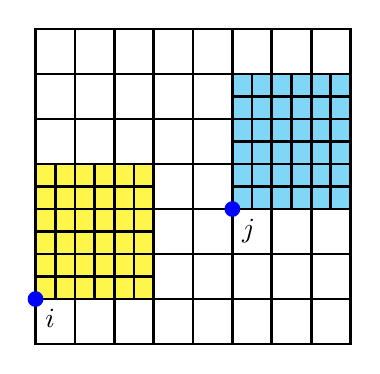
\begin{tikzpicture}[scale=4.0]
    % Define layers
    \pgfdeclarelayer{background}
    \pgfsetlayers{background,main}

    \coordinate (v1_1) at (0.0, 0.0);
    \coordinate (v1_2) at (0.125, 0.0);
    \coordinate (v1_3) at (0.125, 0.14285714285714285);
    \coordinate (v1_4) at (0.0, 0.14285714285714285);
    \draw[black, line width=1.0pt] (v1_1) -- (v1_2) -- (v1_3) -- (v1_4) -- cycle;
    \coordinate (v2_1) at (0.125, 0.0);
    \coordinate (v2_2) at (0.25, 0.0);
    \coordinate (v2_3) at (0.25, 0.14285714285714285);
    \coordinate (v2_4) at (0.125, 0.14285714285714285);
    \draw[black, line width=1.0pt] (v2_1) -- (v2_2) -- (v2_3) -- (v2_4) -- cycle;
    \coordinate (v3_1) at (0.25, 0.0);
    \coordinate (v3_2) at (0.375, 0.0);
    \coordinate (v3_3) at (0.375, 0.14285714285714285);
    \coordinate (v3_4) at (0.25, 0.14285714285714285);
    \draw[black, line width=1.0pt] (v3_1) -- (v3_2) -- (v3_3) -- (v3_4) -- cycle;
    \coordinate (v4_1) at (0.375, 0.0);
    \coordinate (v4_2) at (0.5, 0.0);
    \coordinate (v4_3) at (0.5, 0.14285714285714285);
    \coordinate (v4_4) at (0.375, 0.14285714285714285);
    \draw[black, line width=1.0pt] (v4_1) -- (v4_2) -- (v4_3) -- (v4_4) -- cycle;
    \coordinate (v5_1) at (0.5, 0.0);
    \coordinate (v5_2) at (0.625, 0.0);
    \coordinate (v5_3) at (0.625, 0.14285714285714285);
    \coordinate (v5_4) at (0.5, 0.14285714285714285);
    \draw[black, line width=1.0pt] (v5_1) -- (v5_2) -- (v5_3) -- (v5_4) -- cycle;
    \coordinate (v6_1) at (0.625, 0.0);
    \coordinate (v6_2) at (0.75, 0.0);
    \coordinate (v6_3) at (0.75, 0.14285714285714285);
    \coordinate (v6_4) at (0.625, 0.14285714285714285);
    \draw[black, line width=1.0pt] (v6_1) -- (v6_2) -- (v6_3) -- (v6_4) -- cycle;
    \coordinate (v7_1) at (0.75, 0.0);
    \coordinate (v7_2) at (0.875, 0.0);
    \coordinate (v7_3) at (0.875, 0.14285714285714285);
    \coordinate (v7_4) at (0.75, 0.14285714285714285);
    \draw[black, line width=1.0pt] (v7_1) -- (v7_2) -- (v7_3) -- (v7_4) -- cycle;
    \coordinate (v8_1) at (0.875, 0.0);
    \coordinate (v8_2) at (1.0, 0.0);
    \coordinate (v8_3) at (1.0, 0.14285714285714285);
    \coordinate (v8_4) at (0.875, 0.14285714285714285);
    \draw[black, line width=1.0pt] (v8_1) -- (v8_2) -- (v8_3) -- (v8_4) -- cycle;
    \coordinate (v9_1) at (0.375, 0.14285714285714285);
    \coordinate (v9_2) at (0.5, 0.14285714285714285);
    \coordinate (v9_3) at (0.5, 0.2857142857142857);
    \coordinate (v9_4) at (0.375, 0.2857142857142857);
    \draw[black, line width=1.0pt] (v9_1) -- (v9_2) -- (v9_3) -- (v9_4) -- cycle;
    \coordinate (v10_1) at (0.5, 0.14285714285714285);
    \coordinate (v10_2) at (0.625, 0.14285714285714285);
    \coordinate (v10_3) at (0.625, 0.2857142857142857);
    \coordinate (v10_4) at (0.5, 0.2857142857142857);
    \draw[black, line width=1.0pt] (v10_1) -- (v10_2) -- (v10_3) -- (v10_4) -- cycle;
    \coordinate (v11_1) at (0.625, 0.14285714285714285);
    \coordinate (v11_2) at (0.75, 0.14285714285714285);
    \coordinate (v11_3) at (0.75, 0.2857142857142857);
    \coordinate (v11_4) at (0.625, 0.2857142857142857);
    \draw[black, line width=1.0pt] (v11_1) -- (v11_2) -- (v11_3) -- (v11_4) -- cycle;
    \coordinate (v12_1) at (0.75, 0.14285714285714285);
    \coordinate (v12_2) at (0.875, 0.14285714285714285);
    \coordinate (v12_3) at (0.875, 0.2857142857142857);
    \coordinate (v12_4) at (0.75, 0.2857142857142857);
    \draw[black, line width=1.0pt] (v12_1) -- (v12_2) -- (v12_3) -- (v12_4) -- cycle;
    \coordinate (v13_1) at (0.875, 0.14285714285714285);
    \coordinate (v13_2) at (1.0, 0.14285714285714285);
    \coordinate (v13_3) at (1.0, 0.2857142857142857);
    \coordinate (v13_4) at (0.875, 0.2857142857142857);
    \draw[black, line width=1.0pt] (v13_1) -- (v13_2) -- (v13_3) -- (v13_4) -- cycle;
    \coordinate (v14_1) at (0.375, 0.2857142857142857);
    \coordinate (v14_2) at (0.5, 0.2857142857142857);
    \coordinate (v14_3) at (0.5, 0.42857142857142855);
    \coordinate (v14_4) at (0.375, 0.42857142857142855);
    \draw[black, line width=1.0pt] (v14_1) -- (v14_2) -- (v14_3) -- (v14_4) -- cycle;
    \coordinate (v15_1) at (0.5, 0.2857142857142857);
    \coordinate (v15_2) at (0.625, 0.2857142857142857);
    \coordinate (v15_3) at (0.625, 0.42857142857142855);
    \coordinate (v15_4) at (0.5, 0.42857142857142855);
    \draw[black, line width=1.0pt] (v15_1) -- (v15_2) -- (v15_3) -- (v15_4) -- cycle;
    \coordinate (v16_1) at (0.625, 0.2857142857142857);
    \coordinate (v16_2) at (0.75, 0.2857142857142857);
    \coordinate (v16_3) at (0.75, 0.42857142857142855);
    \coordinate (v16_4) at (0.625, 0.42857142857142855);
    \draw[black, line width=1.0pt] (v16_1) -- (v16_2) -- (v16_3) -- (v16_4) -- cycle;
    \coordinate (v17_1) at (0.75, 0.2857142857142857);
    \coordinate (v17_2) at (0.875, 0.2857142857142857);
    \coordinate (v17_3) at (0.875, 0.42857142857142855);
    \coordinate (v17_4) at (0.75, 0.42857142857142855);
    \draw[black, line width=1.0pt] (v17_1) -- (v17_2) -- (v17_3) -- (v17_4) -- cycle;
    \coordinate (v18_1) at (0.875, 0.2857142857142857);
    \coordinate (v18_2) at (1.0, 0.2857142857142857);
    \coordinate (v18_3) at (1.0, 0.42857142857142855);
    \coordinate (v18_4) at (0.875, 0.42857142857142855);
    \draw[black, line width=1.0pt] (v18_1) -- (v18_2) -- (v18_3) -- (v18_4) -- cycle;
    \coordinate (v19_1) at (0.375, 0.42857142857142855);
    \coordinate (v19_2) at (0.5, 0.42857142857142855);
    \coordinate (v19_3) at (0.5, 0.5714285714285714);
    \coordinate (v19_4) at (0.375, 0.5714285714285714);
    \draw[black, line width=1.0pt] (v19_1) -- (v19_2) -- (v19_3) -- (v19_4) -- cycle;
    \coordinate (v20_1) at (0.5, 0.42857142857142855);
    \coordinate (v20_2) at (0.625, 0.42857142857142855);
    \coordinate (v20_3) at (0.625, 0.5714285714285714);
    \coordinate (v20_4) at (0.5, 0.5714285714285714);
    \draw[black, line width=1.0pt] (v20_1) -- (v20_2) -- (v20_3) -- (v20_4) -- cycle;
    \coordinate (v21_1) at (0.0, 0.5714285714285714);
    \coordinate (v21_2) at (0.125, 0.5714285714285714);
    \coordinate (v21_3) at (0.125, 0.7142857142857143);
    \coordinate (v21_4) at (0.0, 0.7142857142857143);
    \draw[black, line width=1.0pt] (v21_1) -- (v21_2) -- (v21_3) -- (v21_4) -- cycle;
    \coordinate (v22_1) at (0.125, 0.5714285714285714);
    \coordinate (v22_2) at (0.25, 0.5714285714285714);
    \coordinate (v22_3) at (0.25, 0.7142857142857143);
    \coordinate (v22_4) at (0.125, 0.7142857142857143);
    \draw[black, line width=1.0pt] (v22_1) -- (v22_2) -- (v22_3) -- (v22_4) -- cycle;
    \coordinate (v23_1) at (0.25, 0.5714285714285714);
    \coordinate (v23_2) at (0.375, 0.5714285714285714);
    \coordinate (v23_3) at (0.375, 0.7142857142857143);
    \coordinate (v23_4) at (0.25, 0.7142857142857143);
    \draw[black, line width=1.0pt] (v23_1) -- (v23_2) -- (v23_3) -- (v23_4) -- cycle;
    \coordinate (v24_1) at (0.375, 0.5714285714285714);
    \coordinate (v24_2) at (0.5, 0.5714285714285714);
    \coordinate (v24_3) at (0.5, 0.7142857142857143);
    \coordinate (v24_4) at (0.375, 0.7142857142857143);
    \draw[black, line width=1.0pt] (v24_1) -- (v24_2) -- (v24_3) -- (v24_4) -- cycle;
    \coordinate (v25_1) at (0.5, 0.5714285714285714);
    \coordinate (v25_2) at (0.625, 0.5714285714285714);
    \coordinate (v25_3) at (0.625, 0.7142857142857143);
    \coordinate (v25_4) at (0.5, 0.7142857142857143);
    \draw[black, line width=1.0pt] (v25_1) -- (v25_2) -- (v25_3) -- (v25_4) -- cycle;
    \coordinate (v26_1) at (0.0, 0.7142857142857143);
    \coordinate (v26_2) at (0.125, 0.7142857142857143);
    \coordinate (v26_3) at (0.125, 0.8571428571428571);
    \coordinate (v26_4) at (0.0, 0.8571428571428571);
    \draw[black, line width=1.0pt] (v26_1) -- (v26_2) -- (v26_3) -- (v26_4) -- cycle;
    \coordinate (v27_1) at (0.125, 0.7142857142857143);
    \coordinate (v27_2) at (0.25, 0.7142857142857143);
    \coordinate (v27_3) at (0.25, 0.8571428571428571);
    \coordinate (v27_4) at (0.125, 0.8571428571428571);
    \draw[black, line width=1.0pt] (v27_1) -- (v27_2) -- (v27_3) -- (v27_4) -- cycle;
    \coordinate (v28_1) at (0.25, 0.7142857142857143);
    \coordinate (v28_2) at (0.375, 0.7142857142857143);
    \coordinate (v28_3) at (0.375, 0.8571428571428571);
    \coordinate (v28_4) at (0.25, 0.8571428571428571);
    \draw[black, line width=1.0pt] (v28_1) -- (v28_2) -- (v28_3) -- (v28_4) -- cycle;
    \coordinate (v29_1) at (0.375, 0.7142857142857143);
    \coordinate (v29_2) at (0.5, 0.7142857142857143);
    \coordinate (v29_3) at (0.5, 0.8571428571428571);
    \coordinate (v29_4) at (0.375, 0.8571428571428571);
    \draw[black, line width=1.0pt] (v29_1) -- (v29_2) -- (v29_3) -- (v29_4) -- cycle;
    \coordinate (v30_1) at (0.5, 0.7142857142857143);
    \coordinate (v30_2) at (0.625, 0.7142857142857143);
    \coordinate (v30_3) at (0.625, 0.8571428571428571);
    \coordinate (v30_4) at (0.5, 0.8571428571428571);
    \draw[black, line width=1.0pt] (v30_1) -- (v30_2) -- (v30_3) -- (v30_4) -- cycle;
    \coordinate (v31_1) at (0.0, 0.8571428571428571);
    \coordinate (v31_2) at (0.125, 0.8571428571428571);
    \coordinate (v31_3) at (0.125, 1.0);
    \coordinate (v31_4) at (0.0, 1.0);
    \draw[black, line width=1.0pt] (v31_1) -- (v31_2) -- (v31_3) -- (v31_4) -- cycle;
    \coordinate (v32_1) at (0.125, 0.8571428571428571);
    \coordinate (v32_2) at (0.25, 0.8571428571428571);
    \coordinate (v32_3) at (0.25, 1.0);
    \coordinate (v32_4) at (0.125, 1.0);
    \draw[black, line width=1.0pt] (v32_1) -- (v32_2) -- (v32_3) -- (v32_4) -- cycle;
    \coordinate (v33_1) at (0.25, 0.8571428571428571);
    \coordinate (v33_2) at (0.375, 0.8571428571428571);
    \coordinate (v33_3) at (0.375, 1.0);
    \coordinate (v33_4) at (0.25, 1.0);
    \draw[black, line width=1.0pt] (v33_1) -- (v33_2) -- (v33_3) -- (v33_4) -- cycle;
    \coordinate (v34_1) at (0.375, 0.8571428571428571);
    \coordinate (v34_2) at (0.5, 0.8571428571428571);
    \coordinate (v34_3) at (0.5, 1.0);
    \coordinate (v34_4) at (0.375, 1.0);
    \draw[black, line width=1.0pt] (v34_1) -- (v34_2) -- (v34_3) -- (v34_4) -- cycle;
    \coordinate (v35_1) at (0.5, 0.8571428571428571);
    \coordinate (v35_2) at (0.625, 0.8571428571428571);
    \coordinate (v35_3) at (0.625, 1.0);
    \coordinate (v35_4) at (0.5, 1.0);
    \draw[black, line width=1.0pt] (v35_1) -- (v35_2) -- (v35_3) -- (v35_4) -- cycle;
    \coordinate (v36_1) at (0.625, 0.8571428571428571);
    \coordinate (v36_2) at (0.75, 0.8571428571428571);
    \coordinate (v36_3) at (0.75, 1.0);
    \coordinate (v36_4) at (0.625, 1.0);
    \draw[black, line width=1.0pt] (v36_1) -- (v36_2) -- (v36_3) -- (v36_4) -- cycle;
    \coordinate (v37_1) at (0.75, 0.8571428571428571);
    \coordinate (v37_2) at (0.875, 0.8571428571428571);
    \coordinate (v37_3) at (0.875, 1.0);
    \coordinate (v37_4) at (0.75, 1.0);
    \draw[black, line width=1.0pt] (v37_1) -- (v37_2) -- (v37_3) -- (v37_4) -- cycle;
    \coordinate (v38_1) at (0.875, 0.8571428571428571);
    \coordinate (v38_2) at (1.0, 0.8571428571428571);
    \coordinate (v38_3) at (1.0, 1.0);
    \coordinate (v38_4) at (0.875, 1.0);
    \draw[black, line width=1.0pt] (v38_1) -- (v38_2) -- (v38_3) -- (v38_4) -- cycle;
    \coordinate (v39_1) at (0.0, 0.14285714285714285);
    \coordinate (v39_2) at (0.0625, 0.14285714285714285);
    \coordinate (v39_3) at (0.0625, 0.21428571428571427);
    \coordinate (v39_4) at (0.0, 0.21428571428571427);
    \draw[black, line width=1.0pt] (v39_1) -- (v39_2) -- (v39_3) -- (v39_4) -- cycle;
    \coordinate (v40_1) at (0.0625, 0.14285714285714285);
    \coordinate (v40_2) at (0.125, 0.14285714285714285);
    \coordinate (v40_3) at (0.125, 0.21428571428571427);
    \coordinate (v40_4) at (0.0625, 0.21428571428571427);
    \draw[black, line width=1.0pt] (v40_1) -- (v40_2) -- (v40_3) -- (v40_4) -- cycle;
    \coordinate (v41_1) at (0.125, 0.14285714285714285);
    \coordinate (v41_2) at (0.1875, 0.14285714285714285);
    \coordinate (v41_3) at (0.1875, 0.21428571428571427);
    \coordinate (v41_4) at (0.125, 0.21428571428571427);
    \draw[black, line width=1.0pt] (v41_1) -- (v41_2) -- (v41_3) -- (v41_4) -- cycle;
    \coordinate (v42_1) at (0.1875, 0.14285714285714285);
    \coordinate (v42_2) at (0.25, 0.14285714285714285);
    \coordinate (v42_3) at (0.25, 0.21428571428571427);
    \coordinate (v42_4) at (0.1875, 0.21428571428571427);
    \draw[black, line width=1.0pt] (v42_1) -- (v42_2) -- (v42_3) -- (v42_4) -- cycle;
    \coordinate (v43_1) at (0.25, 0.14285714285714285);
    \coordinate (v43_2) at (0.3125, 0.14285714285714285);
    \coordinate (v43_3) at (0.3125, 0.21428571428571427);
    \coordinate (v43_4) at (0.25, 0.21428571428571427);
    \draw[black, line width=1.0pt] (v43_1) -- (v43_2) -- (v43_3) -- (v43_4) -- cycle;
    \coordinate (v44_1) at (0.3125, 0.14285714285714285);
    \coordinate (v44_2) at (0.375, 0.14285714285714285);
    \coordinate (v44_3) at (0.375, 0.21428571428571427);
    \coordinate (v44_4) at (0.3125, 0.21428571428571427);
    \draw[black, line width=1.0pt] (v44_1) -- (v44_2) -- (v44_3) -- (v44_4) -- cycle;
    \coordinate (v45_1) at (0.0, 0.21428571428571427);
    \coordinate (v45_2) at (0.0625, 0.21428571428571427);
    \coordinate (v45_3) at (0.0625, 0.2857142857142857);
    \coordinate (v45_4) at (0.0, 0.2857142857142857);
    \draw[black, line width=1.0pt] (v45_1) -- (v45_2) -- (v45_3) -- (v45_4) -- cycle;
    \coordinate (v46_1) at (0.0625, 0.21428571428571427);
    \coordinate (v46_2) at (0.125, 0.21428571428571427);
    \coordinate (v46_3) at (0.125, 0.2857142857142857);
    \coordinate (v46_4) at (0.0625, 0.2857142857142857);
    \draw[black, line width=1.0pt] (v46_1) -- (v46_2) -- (v46_3) -- (v46_4) -- cycle;
    \coordinate (v47_1) at (0.125, 0.21428571428571427);
    \coordinate (v47_2) at (0.1875, 0.21428571428571427);
    \coordinate (v47_3) at (0.1875, 0.2857142857142857);
    \coordinate (v47_4) at (0.125, 0.2857142857142857);
    \draw[black, line width=1.0pt] (v47_1) -- (v47_2) -- (v47_3) -- (v47_4) -- cycle;
    \coordinate (v48_1) at (0.1875, 0.21428571428571427);
    \coordinate (v48_2) at (0.25, 0.21428571428571427);
    \coordinate (v48_3) at (0.25, 0.2857142857142857);
    \coordinate (v48_4) at (0.1875, 0.2857142857142857);
    \draw[black, line width=1.0pt] (v48_1) -- (v48_2) -- (v48_3) -- (v48_4) -- cycle;
    \coordinate (v49_1) at (0.25, 0.21428571428571427);
    \coordinate (v49_2) at (0.3125, 0.21428571428571427);
    \coordinate (v49_3) at (0.3125, 0.2857142857142857);
    \coordinate (v49_4) at (0.25, 0.2857142857142857);
    \draw[black, line width=1.0pt] (v49_1) -- (v49_2) -- (v49_3) -- (v49_4) -- cycle;
    \coordinate (v50_1) at (0.3125, 0.21428571428571427);
    \coordinate (v50_2) at (0.375, 0.21428571428571427);
    \coordinate (v50_3) at (0.375, 0.2857142857142857);
    \coordinate (v50_4) at (0.3125, 0.2857142857142857);
    \draw[black, line width=1.0pt] (v50_1) -- (v50_2) -- (v50_3) -- (v50_4) -- cycle;
    \coordinate (v51_1) at (0.0, 0.2857142857142857);
    \coordinate (v51_2) at (0.0625, 0.2857142857142857);
    \coordinate (v51_3) at (0.0625, 0.3571428571428571);
    \coordinate (v51_4) at (0.0, 0.3571428571428571);
    \draw[black, line width=1.0pt] (v51_1) -- (v51_2) -- (v51_3) -- (v51_4) -- cycle;
    \coordinate (v52_1) at (0.0625, 0.2857142857142857);
    \coordinate (v52_2) at (0.125, 0.2857142857142857);
    \coordinate (v52_3) at (0.125, 0.3571428571428571);
    \coordinate (v52_4) at (0.0625, 0.3571428571428571);
    \draw[black, line width=1.0pt] (v52_1) -- (v52_2) -- (v52_3) -- (v52_4) -- cycle;
    \coordinate (v53_1) at (0.125, 0.2857142857142857);
    \coordinate (v53_2) at (0.1875, 0.2857142857142857);
    \coordinate (v53_3) at (0.1875, 0.3571428571428571);
    \coordinate (v53_4) at (0.125, 0.3571428571428571);
    \draw[black, line width=1.0pt] (v53_1) -- (v53_2) -- (v53_3) -- (v53_4) -- cycle;
    \coordinate (v54_1) at (0.1875, 0.2857142857142857);
    \coordinate (v54_2) at (0.25, 0.2857142857142857);
    \coordinate (v54_3) at (0.25, 0.3571428571428571);
    \coordinate (v54_4) at (0.1875, 0.3571428571428571);
    \draw[black, line width=1.0pt] (v54_1) -- (v54_2) -- (v54_3) -- (v54_4) -- cycle;
    \coordinate (v55_1) at (0.25, 0.2857142857142857);
    \coordinate (v55_2) at (0.3125, 0.2857142857142857);
    \coordinate (v55_3) at (0.3125, 0.3571428571428571);
    \coordinate (v55_4) at (0.25, 0.3571428571428571);
    \draw[black, line width=1.0pt] (v55_1) -- (v55_2) -- (v55_3) -- (v55_4) -- cycle;
    \coordinate (v56_1) at (0.3125, 0.2857142857142857);
    \coordinate (v56_2) at (0.375, 0.2857142857142857);
    \coordinate (v56_3) at (0.375, 0.3571428571428571);
    \coordinate (v56_4) at (0.3125, 0.3571428571428571);
    \draw[black, line width=1.0pt] (v56_1) -- (v56_2) -- (v56_3) -- (v56_4) -- cycle;
    \coordinate (v57_1) at (0.0, 0.3571428571428571);
    \coordinate (v57_2) at (0.0625, 0.3571428571428571);
    \coordinate (v57_3) at (0.0625, 0.42857142857142855);
    \coordinate (v57_4) at (0.0, 0.42857142857142855);
    \draw[black, line width=1.0pt] (v57_1) -- (v57_2) -- (v57_3) -- (v57_4) -- cycle;
    \coordinate (v58_1) at (0.0625, 0.3571428571428571);
    \coordinate (v58_2) at (0.125, 0.3571428571428571);
    \coordinate (v58_3) at (0.125, 0.42857142857142855);
    \coordinate (v58_4) at (0.0625, 0.42857142857142855);
    \draw[black, line width=1.0pt] (v58_1) -- (v58_2) -- (v58_3) -- (v58_4) -- cycle;
    \coordinate (v59_1) at (0.125, 0.3571428571428571);
    \coordinate (v59_2) at (0.1875, 0.3571428571428571);
    \coordinate (v59_3) at (0.1875, 0.42857142857142855);
    \coordinate (v59_4) at (0.125, 0.42857142857142855);
    \draw[black, line width=1.0pt] (v59_1) -- (v59_2) -- (v59_3) -- (v59_4) -- cycle;
    \coordinate (v60_1) at (0.1875, 0.3571428571428571);
    \coordinate (v60_2) at (0.25, 0.3571428571428571);
    \coordinate (v60_3) at (0.25, 0.42857142857142855);
    \coordinate (v60_4) at (0.1875, 0.42857142857142855);
    \draw[black, line width=1.0pt] (v60_1) -- (v60_2) -- (v60_3) -- (v60_4) -- cycle;
    \coordinate (v61_1) at (0.25, 0.3571428571428571);
    \coordinate (v61_2) at (0.3125, 0.3571428571428571);
    \coordinate (v61_3) at (0.3125, 0.42857142857142855);
    \coordinate (v61_4) at (0.25, 0.42857142857142855);
    \draw[black, line width=1.0pt] (v61_1) -- (v61_2) -- (v61_3) -- (v61_4) -- cycle;
    \coordinate (v62_1) at (0.3125, 0.3571428571428571);
    \coordinate (v62_2) at (0.375, 0.3571428571428571);
    \coordinate (v62_3) at (0.375, 0.42857142857142855);
    \coordinate (v62_4) at (0.3125, 0.42857142857142855);
    \draw[black, line width=1.0pt] (v62_1) -- (v62_2) -- (v62_3) -- (v62_4) -- cycle;
    \coordinate (v63_1) at (0.0, 0.42857142857142855);
    \coordinate (v63_2) at (0.0625, 0.42857142857142855);
    \coordinate (v63_3) at (0.0625, 0.5);
    \coordinate (v63_4) at (0.0, 0.5);
    \draw[black, line width=1.0pt] (v63_1) -- (v63_2) -- (v63_3) -- (v63_4) -- cycle;
    \coordinate (v64_1) at (0.0625, 0.42857142857142855);
    \coordinate (v64_2) at (0.125, 0.42857142857142855);
    \coordinate (v64_3) at (0.125, 0.5);
    \coordinate (v64_4) at (0.0625, 0.5);
    \draw[black, line width=1.0pt] (v64_1) -- (v64_2) -- (v64_3) -- (v64_4) -- cycle;
    \coordinate (v65_1) at (0.125, 0.42857142857142855);
    \coordinate (v65_2) at (0.1875, 0.42857142857142855);
    \coordinate (v65_3) at (0.1875, 0.5);
    \coordinate (v65_4) at (0.125, 0.5);
    \draw[black, line width=1.0pt] (v65_1) -- (v65_2) -- (v65_3) -- (v65_4) -- cycle;
    \coordinate (v66_1) at (0.1875, 0.42857142857142855);
    \coordinate (v66_2) at (0.25, 0.42857142857142855);
    \coordinate (v66_3) at (0.25, 0.5);
    \coordinate (v66_4) at (0.1875, 0.5);
    \draw[black, line width=1.0pt] (v66_1) -- (v66_2) -- (v66_3) -- (v66_4) -- cycle;
    \coordinate (v67_1) at (0.25, 0.42857142857142855);
    \coordinate (v67_2) at (0.3125, 0.42857142857142855);
    \coordinate (v67_3) at (0.3125, 0.5);
    \coordinate (v67_4) at (0.25, 0.5);
    \draw[black, line width=1.0pt] (v67_1) -- (v67_2) -- (v67_3) -- (v67_4) -- cycle;
    \coordinate (v68_1) at (0.3125, 0.42857142857142855);
    \coordinate (v68_2) at (0.375, 0.42857142857142855);
    \coordinate (v68_3) at (0.375, 0.5);
    \coordinate (v68_4) at (0.3125, 0.5);
    \draw[black, line width=1.0pt] (v68_1) -- (v68_2) -- (v68_3) -- (v68_4) -- cycle;
    \coordinate (v69_1) at (0.625, 0.42857142857142855);
    \coordinate (v69_2) at (0.6875, 0.42857142857142855);
    \coordinate (v69_3) at (0.6875, 0.5);
    \coordinate (v69_4) at (0.625, 0.5);
    \draw[black, line width=1.0pt] (v69_1) -- (v69_2) -- (v69_3) -- (v69_4) -- cycle;
    \coordinate (v70_1) at (0.6875, 0.42857142857142855);
    \coordinate (v70_2) at (0.75, 0.42857142857142855);
    \coordinate (v70_3) at (0.75, 0.5);
    \coordinate (v70_4) at (0.6875, 0.5);
    \draw[black, line width=1.0pt] (v70_1) -- (v70_2) -- (v70_3) -- (v70_4) -- cycle;
    \coordinate (v71_1) at (0.75, 0.42857142857142855);
    \coordinate (v71_2) at (0.8125, 0.42857142857142855);
    \coordinate (v71_3) at (0.8125, 0.5);
    \coordinate (v71_4) at (0.75, 0.5);
    \draw[black, line width=1.0pt] (v71_1) -- (v71_2) -- (v71_3) -- (v71_4) -- cycle;
    \coordinate (v72_1) at (0.8125, 0.42857142857142855);
    \coordinate (v72_2) at (0.875, 0.42857142857142855);
    \coordinate (v72_3) at (0.875, 0.5);
    \coordinate (v72_4) at (0.8125, 0.5);
    \draw[black, line width=1.0pt] (v72_1) -- (v72_2) -- (v72_3) -- (v72_4) -- cycle;
    \coordinate (v73_1) at (0.875, 0.42857142857142855);
    \coordinate (v73_2) at (0.9375, 0.42857142857142855);
    \coordinate (v73_3) at (0.9375, 0.5);
    \coordinate (v73_4) at (0.875, 0.5);
    \draw[black, line width=1.0pt] (v73_1) -- (v73_2) -- (v73_3) -- (v73_4) -- cycle;
    \coordinate (v74_1) at (0.9375, 0.42857142857142855);
    \coordinate (v74_2) at (1.0, 0.42857142857142855);
    \coordinate (v74_3) at (1.0, 0.5);
    \coordinate (v74_4) at (0.9375, 0.5);
    \draw[black, line width=1.0pt] (v74_1) -- (v74_2) -- (v74_3) -- (v74_4) -- cycle;
    \coordinate (v75_1) at (0.0, 0.5);
    \coordinate (v75_2) at (0.0625, 0.5);
    \coordinate (v75_3) at (0.0625, 0.5714285714285714);
    \coordinate (v75_4) at (0.0, 0.5714285714285714);
    \draw[black, line width=1.0pt] (v75_1) -- (v75_2) -- (v75_3) -- (v75_4) -- cycle;
    \coordinate (v76_1) at (0.0625, 0.5);
    \coordinate (v76_2) at (0.125, 0.5);
    \coordinate (v76_3) at (0.125, 0.5714285714285714);
    \coordinate (v76_4) at (0.0625, 0.5714285714285714);
    \draw[black, line width=1.0pt] (v76_1) -- (v76_2) -- (v76_3) -- (v76_4) -- cycle;
    \coordinate (v77_1) at (0.125, 0.5);
    \coordinate (v77_2) at (0.1875, 0.5);
    \coordinate (v77_3) at (0.1875, 0.5714285714285714);
    \coordinate (v77_4) at (0.125, 0.5714285714285714);
    \draw[black, line width=1.0pt] (v77_1) -- (v77_2) -- (v77_3) -- (v77_4) -- cycle;
    \coordinate (v78_1) at (0.1875, 0.5);
    \coordinate (v78_2) at (0.25, 0.5);
    \coordinate (v78_3) at (0.25, 0.5714285714285714);
    \coordinate (v78_4) at (0.1875, 0.5714285714285714);
    \draw[black, line width=1.0pt] (v78_1) -- (v78_2) -- (v78_3) -- (v78_4) -- cycle;
    \coordinate (v79_1) at (0.25, 0.5);
    \coordinate (v79_2) at (0.3125, 0.5);
    \coordinate (v79_3) at (0.3125, 0.5714285714285714);
    \coordinate (v79_4) at (0.25, 0.5714285714285714);
    \draw[black, line width=1.0pt] (v79_1) -- (v79_2) -- (v79_3) -- (v79_4) -- cycle;
    \coordinate (v80_1) at (0.3125, 0.5);
    \coordinate (v80_2) at (0.375, 0.5);
    \coordinate (v80_3) at (0.375, 0.5714285714285714);
    \coordinate (v80_4) at (0.3125, 0.5714285714285714);
    \draw[black, line width=1.0pt] (v80_1) -- (v80_2) -- (v80_3) -- (v80_4) -- cycle;
    \coordinate (v81_1) at (0.625, 0.5);
    \coordinate (v81_2) at (0.6875, 0.5);
    \coordinate (v81_3) at (0.6875, 0.5714285714285714);
    \coordinate (v81_4) at (0.625, 0.5714285714285714);
    \draw[black, line width=1.0pt] (v81_1) -- (v81_2) -- (v81_3) -- (v81_4) -- cycle;
    \coordinate (v82_1) at (0.6875, 0.5);
    \coordinate (v82_2) at (0.75, 0.5);
    \coordinate (v82_3) at (0.75, 0.5714285714285714);
    \coordinate (v82_4) at (0.6875, 0.5714285714285714);
    \draw[black, line width=1.0pt] (v82_1) -- (v82_2) -- (v82_3) -- (v82_4) -- cycle;
    \coordinate (v83_1) at (0.75, 0.5);
    \coordinate (v83_2) at (0.8125, 0.5);
    \coordinate (v83_3) at (0.8125, 0.5714285714285714);
    \coordinate (v83_4) at (0.75, 0.5714285714285714);
    \draw[black, line width=1.0pt] (v83_1) -- (v83_2) -- (v83_3) -- (v83_4) -- cycle;
    \coordinate (v84_1) at (0.8125, 0.5);
    \coordinate (v84_2) at (0.875, 0.5);
    \coordinate (v84_3) at (0.875, 0.5714285714285714);
    \coordinate (v84_4) at (0.8125, 0.5714285714285714);
    \draw[black, line width=1.0pt] (v84_1) -- (v84_2) -- (v84_3) -- (v84_4) -- cycle;
    \coordinate (v85_1) at (0.875, 0.5);
    \coordinate (v85_2) at (0.9375, 0.5);
    \coordinate (v85_3) at (0.9375, 0.5714285714285714);
    \coordinate (v85_4) at (0.875, 0.5714285714285714);
    \draw[black, line width=1.0pt] (v85_1) -- (v85_2) -- (v85_3) -- (v85_4) -- cycle;
    \coordinate (v86_1) at (0.9375, 0.5);
    \coordinate (v86_2) at (1.0, 0.5);
    \coordinate (v86_3) at (1.0, 0.5714285714285714);
    \coordinate (v86_4) at (0.9375, 0.5714285714285714);
    \draw[black, line width=1.0pt] (v86_1) -- (v86_2) -- (v86_3) -- (v86_4) -- cycle;
    \coordinate (v87_1) at (0.625, 0.5714285714285714);
    \coordinate (v87_2) at (0.6875, 0.5714285714285714);
    \coordinate (v87_3) at (0.6875, 0.6428571428571428);
    \coordinate (v87_4) at (0.625, 0.6428571428571428);
    \draw[black, line width=1.0pt] (v87_1) -- (v87_2) -- (v87_3) -- (v87_4) -- cycle;
    \coordinate (v88_1) at (0.6875, 0.5714285714285714);
    \coordinate (v88_2) at (0.75, 0.5714285714285714);
    \coordinate (v88_3) at (0.75, 0.6428571428571428);
    \coordinate (v88_4) at (0.6875, 0.6428571428571428);
    \draw[black, line width=1.0pt] (v88_1) -- (v88_2) -- (v88_3) -- (v88_4) -- cycle;
    \coordinate (v89_1) at (0.75, 0.5714285714285714);
    \coordinate (v89_2) at (0.8125, 0.5714285714285714);
    \coordinate (v89_3) at (0.8125, 0.6428571428571428);
    \coordinate (v89_4) at (0.75, 0.6428571428571428);
    \draw[black, line width=1.0pt] (v89_1) -- (v89_2) -- (v89_3) -- (v89_4) -- cycle;
    \coordinate (v90_1) at (0.8125, 0.5714285714285714);
    \coordinate (v90_2) at (0.875, 0.5714285714285714);
    \coordinate (v90_3) at (0.875, 0.6428571428571428);
    \coordinate (v90_4) at (0.8125, 0.6428571428571428);
    \draw[black, line width=1.0pt] (v90_1) -- (v90_2) -- (v90_3) -- (v90_4) -- cycle;
    \coordinate (v91_1) at (0.875, 0.5714285714285714);
    \coordinate (v91_2) at (0.9375, 0.5714285714285714);
    \coordinate (v91_3) at (0.9375, 0.6428571428571428);
    \coordinate (v91_4) at (0.875, 0.6428571428571428);
    \draw[black, line width=1.0pt] (v91_1) -- (v91_2) -- (v91_3) -- (v91_4) -- cycle;
    \coordinate (v92_1) at (0.9375, 0.5714285714285714);
    \coordinate (v92_2) at (1.0, 0.5714285714285714);
    \coordinate (v92_3) at (1.0, 0.6428571428571428);
    \coordinate (v92_4) at (0.9375, 0.6428571428571428);
    \draw[black, line width=1.0pt] (v92_1) -- (v92_2) -- (v92_3) -- (v92_4) -- cycle;
    \coordinate (v93_1) at (0.625, 0.6428571428571428);
    \coordinate (v93_2) at (0.6875, 0.6428571428571428);
    \coordinate (v93_3) at (0.6875, 0.7142857142857143);
    \coordinate (v93_4) at (0.625, 0.7142857142857143);
    \draw[black, line width=1.0pt] (v93_1) -- (v93_2) -- (v93_3) -- (v93_4) -- cycle;
    \coordinate (v94_1) at (0.6875, 0.6428571428571428);
    \coordinate (v94_2) at (0.75, 0.6428571428571428);
    \coordinate (v94_3) at (0.75, 0.7142857142857143);
    \coordinate (v94_4) at (0.6875, 0.7142857142857143);
    \draw[black, line width=1.0pt] (v94_1) -- (v94_2) -- (v94_3) -- (v94_4) -- cycle;
    \coordinate (v95_1) at (0.75, 0.6428571428571428);
    \coordinate (v95_2) at (0.8125, 0.6428571428571428);
    \coordinate (v95_3) at (0.8125, 0.7142857142857143);
    \coordinate (v95_4) at (0.75, 0.7142857142857143);
    \draw[black, line width=1.0pt] (v95_1) -- (v95_2) -- (v95_3) -- (v95_4) -- cycle;
    \coordinate (v96_1) at (0.8125, 0.6428571428571428);
    \coordinate (v96_2) at (0.875, 0.6428571428571428);
    \coordinate (v96_3) at (0.875, 0.7142857142857143);
    \coordinate (v96_4) at (0.8125, 0.7142857142857143);
    \draw[black, line width=1.0pt] (v96_1) -- (v96_2) -- (v96_3) -- (v96_4) -- cycle;
    \coordinate (v97_1) at (0.875, 0.6428571428571428);
    \coordinate (v97_2) at (0.9375, 0.6428571428571428);
    \coordinate (v97_3) at (0.9375, 0.7142857142857143);
    \coordinate (v97_4) at (0.875, 0.7142857142857143);
    \draw[black, line width=1.0pt] (v97_1) -- (v97_2) -- (v97_3) -- (v97_4) -- cycle;
    \coordinate (v98_1) at (0.9375, 0.6428571428571428);
    \coordinate (v98_2) at (1.0, 0.6428571428571428);
    \coordinate (v98_3) at (1.0, 0.7142857142857143);
    \coordinate (v98_4) at (0.9375, 0.7142857142857143);
    \draw[black, line width=1.0pt] (v98_1) -- (v98_2) -- (v98_3) -- (v98_4) -- cycle;
    \coordinate (v99_1) at (0.625, 0.7142857142857143);
    \coordinate (v99_2) at (0.6875, 0.7142857142857143);
    \coordinate (v99_3) at (0.6875, 0.7857142857142857);
    \coordinate (v99_4) at (0.625, 0.7857142857142857);
    \draw[black, line width=1.0pt] (v99_1) -- (v99_2) -- (v99_3) -- (v99_4) -- cycle;
    \coordinate (v100_1) at (0.6875, 0.7142857142857143);
    \coordinate (v100_2) at (0.75, 0.7142857142857143);
    \coordinate (v100_3) at (0.75, 0.7857142857142857);
    \coordinate (v100_4) at (0.6875, 0.7857142857142857);
    \draw[black, line width=1.0pt] (v100_1) -- (v100_2) -- (v100_3) -- (v100_4) -- cycle;
    \coordinate (v101_1) at (0.75, 0.7142857142857143);
    \coordinate (v101_2) at (0.8125, 0.7142857142857143);
    \coordinate (v101_3) at (0.8125, 0.7857142857142857);
    \coordinate (v101_4) at (0.75, 0.7857142857142857);
    \draw[black, line width=1.0pt] (v101_1) -- (v101_2) -- (v101_3) -- (v101_4) -- cycle;
    \coordinate (v102_1) at (0.8125, 0.7142857142857143);
    \coordinate (v102_2) at (0.875, 0.7142857142857143);
    \coordinate (v102_3) at (0.875, 0.7857142857142857);
    \coordinate (v102_4) at (0.8125, 0.7857142857142857);
    \draw[black, line width=1.0pt] (v102_1) -- (v102_2) -- (v102_3) -- (v102_4) -- cycle;
    \coordinate (v103_1) at (0.875, 0.7142857142857143);
    \coordinate (v103_2) at (0.9375, 0.7142857142857143);
    \coordinate (v103_3) at (0.9375, 0.7857142857142857);
    \coordinate (v103_4) at (0.875, 0.7857142857142857);
    \draw[black, line width=1.0pt] (v103_1) -- (v103_2) -- (v103_3) -- (v103_4) -- cycle;
    \coordinate (v104_1) at (0.9375, 0.7142857142857143);
    \coordinate (v104_2) at (1.0, 0.7142857142857143);
    \coordinate (v104_3) at (1.0, 0.7857142857142857);
    \coordinate (v104_4) at (0.9375, 0.7857142857142857);
    \draw[black, line width=1.0pt] (v104_1) -- (v104_2) -- (v104_3) -- (v104_4) -- cycle;
    \coordinate (v105_1) at (0.625, 0.7857142857142857);
    \coordinate (v105_2) at (0.6875, 0.7857142857142857);
    \coordinate (v105_3) at (0.6875, 0.8571428571428571);
    \coordinate (v105_4) at (0.625, 0.8571428571428571);
    \draw[black, line width=1.0pt] (v105_1) -- (v105_2) -- (v105_3) -- (v105_4) -- cycle;
    \coordinate (v106_1) at (0.6875, 0.7857142857142857);
    \coordinate (v106_2) at (0.75, 0.7857142857142857);
    \coordinate (v106_3) at (0.75, 0.8571428571428571);
    \coordinate (v106_4) at (0.6875, 0.8571428571428571);
    \draw[black, line width=1.0pt] (v106_1) -- (v106_2) -- (v106_3) -- (v106_4) -- cycle;
    \coordinate (v107_1) at (0.75, 0.7857142857142857);
    \coordinate (v107_2) at (0.8125, 0.7857142857142857);
    \coordinate (v107_3) at (0.8125, 0.8571428571428571);
    \coordinate (v107_4) at (0.75, 0.8571428571428571);
    \draw[black, line width=1.0pt] (v107_1) -- (v107_2) -- (v107_3) -- (v107_4) -- cycle;
    \coordinate (v108_1) at (0.8125, 0.7857142857142857);
    \coordinate (v108_2) at (0.875, 0.7857142857142857);
    \coordinate (v108_3) at (0.875, 0.8571428571428571);
    \coordinate (v108_4) at (0.8125, 0.8571428571428571);
    \draw[black, line width=1.0pt] (v108_1) -- (v108_2) -- (v108_3) -- (v108_4) -- cycle;
    \coordinate (v109_1) at (0.875, 0.7857142857142857);
    \coordinate (v109_2) at (0.9375, 0.7857142857142857);
    \coordinate (v109_3) at (0.9375, 0.8571428571428571);
    \coordinate (v109_4) at (0.875, 0.8571428571428571);
    \draw[black, line width=1.0pt] (v109_1) -- (v109_2) -- (v109_3) -- (v109_4) -- cycle;
    \coordinate (v110_1) at (0.9375, 0.7857142857142857);
    \coordinate (v110_2) at (1.0, 0.7857142857142857);
    \coordinate (v110_3) at (1.0, 0.8571428571428571);
    \coordinate (v110_4) at (0.9375, 0.8571428571428571);
    \draw[black, line width=1.0pt] (v110_1) -- (v110_2) -- (v110_3) -- (v110_4) -- cycle;

    % Fill the pair support
    \begin{pgfonlayer}{background}
        \fill[yellow, opacity=0.7] (v1_4) rectangle (v19_4);
        \fill[cyan, opacity=0.5] (v20_2) rectangle (v38_2);
    \end{pgfonlayer}

    \node[anchor=north west] at (v1_4) {\(\boldvec{i}\)};
    \node[anchor=north west] at (v20_2) {\(\boldvec{j}\)};
    
    \fill[blue] (v1_4) circle (0.025);
    \fill[blue] (v20_2) circle (0.025);
\end{tikzpicture}

        \caption{}
        \label{fig:problematic-pair-algorithm-case-1-illustration}
    \end{subfigure}
	\hfill
    \begin{subfigure}[t]{0.325\textwidth}
		\centering
		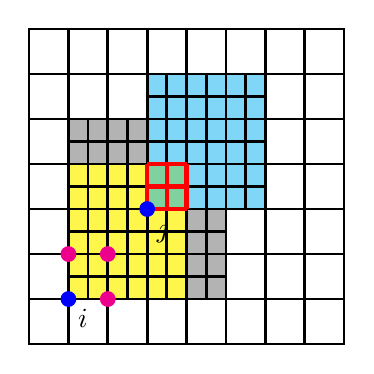
\begin{tikzpicture}[scale=4.0]
    % Define layers
    \pgfdeclarelayer{background}
    \pgfsetlayers{background,main}
    
    \coordinate (v1_1) at (0.0, 0.0);
    \coordinate (v1_2) at (0.125, 0.0);
    \coordinate (v1_3) at (0.125, 0.14285714285714285);
    \coordinate (v1_4) at (0.0, 0.14285714285714285);
    \draw[black, line width=1.0pt] (v1_1) -- (v1_2) -- (v1_3) -- (v1_4) -- cycle;
    \coordinate (v2_1) at (0.125, 0.0);
    \coordinate (v2_2) at (0.25, 0.0);
    \coordinate (v2_3) at (0.25, 0.14285714285714285);
    \coordinate (v2_4) at (0.125, 0.14285714285714285);
    \draw[black, line width=1.0pt] (v2_1) -- (v2_2) -- (v2_3) -- (v2_4) -- cycle;
    \coordinate (v3_1) at (0.25, 0.0);
    \coordinate (v3_2) at (0.375, 0.0);
    \coordinate (v3_3) at (0.375, 0.14285714285714285);
    \coordinate (v3_4) at (0.25, 0.14285714285714285);
    \draw[black, line width=1.0pt] (v3_1) -- (v3_2) -- (v3_3) -- (v3_4) -- cycle;
    \coordinate (v4_1) at (0.375, 0.0);
    \coordinate (v4_2) at (0.5, 0.0);
    \coordinate (v4_3) at (0.5, 0.14285714285714285);
    \coordinate (v4_4) at (0.375, 0.14285714285714285);
    \draw[black, line width=1.0pt] (v4_1) -- (v4_2) -- (v4_3) -- (v4_4) -- cycle;
    \coordinate (v5_1) at (0.5, 0.0);
    \coordinate (v5_2) at (0.625, 0.0);
    \coordinate (v5_3) at (0.625, 0.14285714285714285);
    \coordinate (v5_4) at (0.5, 0.14285714285714285);
    \draw[black, line width=1.0pt] (v5_1) -- (v5_2) -- (v5_3) -- (v5_4) -- cycle;
    \coordinate (v6_1) at (0.625, 0.0);
    \coordinate (v6_2) at (0.75, 0.0);
    \coordinate (v6_3) at (0.75, 0.14285714285714285);
    \coordinate (v6_4) at (0.625, 0.14285714285714285);
    \draw[black, line width=1.0pt] (v6_1) -- (v6_2) -- (v6_3) -- (v6_4) -- cycle;
    \coordinate (v7_1) at (0.75, 0.0);
    \coordinate (v7_2) at (0.875, 0.0);
    \coordinate (v7_3) at (0.875, 0.14285714285714285);
    \coordinate (v7_4) at (0.75, 0.14285714285714285);
    \draw[black, line width=1.0pt] (v7_1) -- (v7_2) -- (v7_3) -- (v7_4) -- cycle;
    \coordinate (v8_1) at (0.875, 0.0);
    \coordinate (v8_2) at (1.0, 0.0);
    \coordinate (v8_3) at (1.0, 0.14285714285714285);
    \coordinate (v8_4) at (0.875, 0.14285714285714285);
    \draw[black, line width=1.0pt] (v8_1) -- (v8_2) -- (v8_3) -- (v8_4) -- cycle;
    \coordinate (v9_1) at (0.0, 0.14285714285714285);
    \coordinate (v9_2) at (0.125, 0.14285714285714285);
    \coordinate (v9_3) at (0.125, 0.2857142857142857);
    \coordinate (v9_4) at (0.0, 0.2857142857142857);
    \draw[black, line width=1.0pt] (v9_1) -- (v9_2) -- (v9_3) -- (v9_4) -- cycle;
    \coordinate (v10_1) at (0.625, 0.14285714285714285);
    \coordinate (v10_2) at (0.75, 0.14285714285714285);
    \coordinate (v10_3) at (0.75, 0.2857142857142857);
    \coordinate (v10_4) at (0.625, 0.2857142857142857);
    \draw[black, line width=1.0pt] (v10_1) -- (v10_2) -- (v10_3) -- (v10_4) -- cycle;
    \coordinate (v11_1) at (0.75, 0.14285714285714285);
    \coordinate (v11_2) at (0.875, 0.14285714285714285);
    \coordinate (v11_3) at (0.875, 0.2857142857142857);
    \coordinate (v11_4) at (0.75, 0.2857142857142857);
    \draw[black, line width=1.0pt] (v11_1) -- (v11_2) -- (v11_3) -- (v11_4) -- cycle;
    \coordinate (v12_1) at (0.875, 0.14285714285714285);
    \coordinate (v12_2) at (1.0, 0.14285714285714285);
    \coordinate (v12_3) at (1.0, 0.2857142857142857);
    \coordinate (v12_4) at (0.875, 0.2857142857142857);
    \draw[black, line width=1.0pt] (v12_1) -- (v12_2) -- (v12_3) -- (v12_4) -- cycle;
    \coordinate (v13_1) at (0.0, 0.2857142857142857);
    \coordinate (v13_2) at (0.125, 0.2857142857142857);
    \coordinate (v13_3) at (0.125, 0.42857142857142855);
    \coordinate (v13_4) at (0.0, 0.42857142857142855);
    \draw[black, line width=1.0pt] (v13_1) -- (v13_2) -- (v13_3) -- (v13_4) -- cycle;
    \coordinate (v14_1) at (0.625, 0.2857142857142857);
    \coordinate (v14_2) at (0.75, 0.2857142857142857);
    \coordinate (v14_3) at (0.75, 0.42857142857142855);
    \coordinate (v14_4) at (0.625, 0.42857142857142855);
    \draw[black, line width=1.0pt] (v14_1) -- (v14_2) -- (v14_3) -- (v14_4) -- cycle;
    \coordinate (v15_1) at (0.75, 0.2857142857142857);
    \coordinate (v15_2) at (0.875, 0.2857142857142857);
    \coordinate (v15_3) at (0.875, 0.42857142857142855);
    \coordinate (v15_4) at (0.75, 0.42857142857142855);
    \draw[black, line width=1.0pt] (v15_1) -- (v15_2) -- (v15_3) -- (v15_4) -- cycle;
    \coordinate (v16_1) at (0.875, 0.2857142857142857);
    \coordinate (v16_2) at (1.0, 0.2857142857142857);
    \coordinate (v16_3) at (1.0, 0.42857142857142855);
    \coordinate (v16_4) at (0.875, 0.42857142857142855);
    \draw[black, line width=1.0pt] (v16_1) -- (v16_2) -- (v16_3) -- (v16_4) -- cycle;
    \coordinate (v17_1) at (0.0, 0.42857142857142855);
    \coordinate (v17_2) at (0.125, 0.42857142857142855);
    \coordinate (v17_3) at (0.125, 0.5714285714285714);
    \coordinate (v17_4) at (0.0, 0.5714285714285714);
    \draw[black, line width=1.0pt] (v17_1) -- (v17_2) -- (v17_3) -- (v17_4) -- cycle;
    \coordinate (v18_1) at (0.75, 0.42857142857142855);
    \coordinate (v18_2) at (0.875, 0.42857142857142855);
    \coordinate (v18_3) at (0.875, 0.5714285714285714);
    \coordinate (v18_4) at (0.75, 0.5714285714285714);
    \draw[black, line width=1.0pt] (v18_1) -- (v18_2) -- (v18_3) -- (v18_4) -- cycle;
    \coordinate (v19_1) at (0.875, 0.42857142857142855);
    \coordinate (v19_2) at (1.0, 0.42857142857142855);
    \coordinate (v19_3) at (1.0, 0.5714285714285714);
    \coordinate (v19_4) at (0.875, 0.5714285714285714);
    \draw[black, line width=1.0pt] (v19_1) -- (v19_2) -- (v19_3) -- (v19_4) -- cycle;
    \coordinate (v20_1) at (0.0, 0.5714285714285714);
    \coordinate (v20_2) at (0.125, 0.5714285714285714);
    \coordinate (v20_3) at (0.125, 0.7142857142857143);
    \coordinate (v20_4) at (0.0, 0.7142857142857143);
    \draw[black, line width=1.0pt] (v20_1) -- (v20_2) -- (v20_3) -- (v20_4) -- cycle;
    \coordinate (v21_1) at (0.75, 0.5714285714285714);
    \coordinate (v21_2) at (0.875, 0.5714285714285714);
    \coordinate (v21_3) at (0.875, 0.7142857142857143);
    \coordinate (v21_4) at (0.75, 0.7142857142857143);
    \draw[black, line width=1.0pt] (v21_1) -- (v21_2) -- (v21_3) -- (v21_4) -- cycle;
    \coordinate (v22_1) at (0.875, 0.5714285714285714);
    \coordinate (v22_2) at (1.0, 0.5714285714285714);
    \coordinate (v22_3) at (1.0, 0.7142857142857143);
    \coordinate (v22_4) at (0.875, 0.7142857142857143);
    \draw[black, line width=1.0pt] (v22_1) -- (v22_2) -- (v22_3) -- (v22_4) -- cycle;
    \coordinate (v23_1) at (0.0, 0.7142857142857143);
    \coordinate (v23_2) at (0.125, 0.7142857142857143);
    \coordinate (v23_3) at (0.125, 0.8571428571428571);
    \coordinate (v23_4) at (0.0, 0.8571428571428571);
    \draw[black, line width=1.0pt] (v23_1) -- (v23_2) -- (v23_3) -- (v23_4) -- cycle;
    \coordinate (v24_1) at (0.125, 0.7142857142857143);
    \coordinate (v24_2) at (0.25, 0.7142857142857143);
    \coordinate (v24_3) at (0.25, 0.8571428571428571);
    \coordinate (v24_4) at (0.125, 0.8571428571428571);
    \draw[black, line width=1.0pt] (v24_1) -- (v24_2) -- (v24_3) -- (v24_4) -- cycle;
    \coordinate (v25_1) at (0.25, 0.7142857142857143);
    \coordinate (v25_2) at (0.375, 0.7142857142857143);
    \coordinate (v25_3) at (0.375, 0.8571428571428571);
    \coordinate (v25_4) at (0.25, 0.8571428571428571);
    \draw[black, line width=1.0pt] (v25_1) -- (v25_2) -- (v25_3) -- (v25_4) -- cycle;
    \coordinate (v26_1) at (0.75, 0.7142857142857143);
    \coordinate (v26_2) at (0.875, 0.7142857142857143);
    \coordinate (v26_3) at (0.875, 0.8571428571428571);
    \coordinate (v26_4) at (0.75, 0.8571428571428571);
    \draw[black, line width=1.0pt] (v26_1) -- (v26_2) -- (v26_3) -- (v26_4) -- cycle;
    \coordinate (v27_1) at (0.875, 0.7142857142857143);
    \coordinate (v27_2) at (1.0, 0.7142857142857143);
    \coordinate (v27_3) at (1.0, 0.8571428571428571);
    \coordinate (v27_4) at (0.875, 0.8571428571428571);
    \draw[black, line width=1.0pt] (v27_1) -- (v27_2) -- (v27_3) -- (v27_4) -- cycle;
    \coordinate (v28_1) at (0.0, 0.8571428571428571);
    \coordinate (v28_2) at (0.125, 0.8571428571428571);
    \coordinate (v28_3) at (0.125, 1.0);
    \coordinate (v28_4) at (0.0, 1.0);
    \draw[black, line width=1.0pt] (v28_1) -- (v28_2) -- (v28_3) -- (v28_4) -- cycle;
    \coordinate (v29_1) at (0.125, 0.8571428571428571);
    \coordinate (v29_2) at (0.25, 0.8571428571428571);
    \coordinate (v29_3) at (0.25, 1.0);
    \coordinate (v29_4) at (0.125, 1.0);
    \draw[black, line width=1.0pt] (v29_1) -- (v29_2) -- (v29_3) -- (v29_4) -- cycle;
    \coordinate (v30_1) at (0.25, 0.8571428571428571);
    \coordinate (v30_2) at (0.375, 0.8571428571428571);
    \coordinate (v30_3) at (0.375, 1.0);
    \coordinate (v30_4) at (0.25, 1.0);
    \draw[black, line width=1.0pt] (v30_1) -- (v30_2) -- (v30_3) -- (v30_4) -- cycle;
    \coordinate (v31_1) at (0.375, 0.8571428571428571);
    \coordinate (v31_2) at (0.5, 0.8571428571428571);
    \coordinate (v31_3) at (0.5, 1.0);
    \coordinate (v31_4) at (0.375, 1.0);
    \draw[black, line width=1.0pt] (v31_1) -- (v31_2) -- (v31_3) -- (v31_4) -- cycle;
    \coordinate (v32_1) at (0.5, 0.8571428571428571);
    \coordinate (v32_2) at (0.625, 0.8571428571428571);
    \coordinate (v32_3) at (0.625, 1.0);
    \coordinate (v32_4) at (0.5, 1.0);
    \draw[black, line width=1.0pt] (v32_1) -- (v32_2) -- (v32_3) -- (v32_4) -- cycle;
    \coordinate (v33_1) at (0.625, 0.8571428571428571);
    \coordinate (v33_2) at (0.75, 0.8571428571428571);
    \coordinate (v33_3) at (0.75, 1.0);
    \coordinate (v33_4) at (0.625, 1.0);
    \draw[black, line width=1.0pt] (v33_1) -- (v33_2) -- (v33_3) -- (v33_4) -- cycle;
    \coordinate (v34_1) at (0.75, 0.8571428571428571);
    \coordinate (v34_2) at (0.875, 0.8571428571428571);
    \coordinate (v34_3) at (0.875, 1.0);
    \coordinate (v34_4) at (0.75, 1.0);
    \draw[black, line width=1.0pt] (v34_1) -- (v34_2) -- (v34_3) -- (v34_4) -- cycle;
    \coordinate (v35_1) at (0.875, 0.8571428571428571);
    \coordinate (v35_2) at (1.0, 0.8571428571428571);
    \coordinate (v35_3) at (1.0, 1.0);
    \coordinate (v35_4) at (0.875, 1.0);
    \draw[black, line width=1.0pt] (v35_1) -- (v35_2) -- (v35_3) -- (v35_4) -- cycle;
    \coordinate (v36_1) at (0.125, 0.14285714285714285);
    \coordinate (v36_2) at (0.1875, 0.14285714285714285);
    \coordinate (v36_3) at (0.1875, 0.21428571428571427);
    \coordinate (v36_4) at (0.125, 0.21428571428571427);
    \draw[black, line width=1.0pt] (v36_1) -- (v36_2) -- (v36_3) -- (v36_4) -- cycle;
    \coordinate (v37_1) at (0.1875, 0.14285714285714285);
    \coordinate (v37_2) at (0.25, 0.14285714285714285);
    \coordinate (v37_3) at (0.25, 0.21428571428571427);
    \coordinate (v37_4) at (0.1875, 0.21428571428571427);
    \draw[black, line width=1.0pt] (v37_1) -- (v37_2) -- (v37_3) -- (v37_4) -- cycle;
    \coordinate (v38_1) at (0.25, 0.14285714285714285);
    \coordinate (v38_2) at (0.3125, 0.14285714285714285);
    \coordinate (v38_3) at (0.3125, 0.21428571428571427);
    \coordinate (v38_4) at (0.25, 0.21428571428571427);
    \draw[black, line width=1.0pt] (v38_1) -- (v38_2) -- (v38_3) -- (v38_4) -- cycle;
    \coordinate (v39_1) at (0.3125, 0.14285714285714285);
    \coordinate (v39_2) at (0.375, 0.14285714285714285);
    \coordinate (v39_3) at (0.375, 0.21428571428571427);
    \coordinate (v39_4) at (0.3125, 0.21428571428571427);
    \draw[black, line width=1.0pt] (v39_1) -- (v39_2) -- (v39_3) -- (v39_4) -- cycle;
    \coordinate (v40_1) at (0.375, 0.14285714285714285);
    \coordinate (v40_2) at (0.4375, 0.14285714285714285);
    \coordinate (v40_3) at (0.4375, 0.21428571428571427);
    \coordinate (v40_4) at (0.375, 0.21428571428571427);
    \draw[black, line width=1.0pt] (v40_1) -- (v40_2) -- (v40_3) -- (v40_4) -- cycle;
    \coordinate (v41_1) at (0.4375, 0.14285714285714285);
    \coordinate (v41_2) at (0.5, 0.14285714285714285);
    \coordinate (v41_3) at (0.5, 0.21428571428571427);
    \coordinate (v41_4) at (0.4375, 0.21428571428571427);
    \draw[black, line width=1.0pt] (v41_1) -- (v41_2) -- (v41_3) -- (v41_4) -- cycle;
    \coordinate (v42_1) at (0.5, 0.14285714285714285);
    \coordinate (v42_2) at (0.5625, 0.14285714285714285);
    \coordinate (v42_3) at (0.5625, 0.21428571428571427);
    \coordinate (v42_4) at (0.5, 0.21428571428571427);
    \draw[black, line width=1.0pt] (v42_1) -- (v42_2) -- (v42_3) -- (v42_4) -- cycle;
    \coordinate (v43_1) at (0.5625, 0.14285714285714285);
    \coordinate (v43_2) at (0.625, 0.14285714285714285);
    \coordinate (v43_3) at (0.625, 0.21428571428571427);
    \coordinate (v43_4) at (0.5625, 0.21428571428571427);
    \draw[black, line width=1.0pt] (v43_1) -- (v43_2) -- (v43_3) -- (v43_4) -- cycle;
    \coordinate (v44_1) at (0.125, 0.21428571428571427);
    \coordinate (v44_2) at (0.1875, 0.21428571428571427);
    \coordinate (v44_3) at (0.1875, 0.2857142857142857);
    \coordinate (v44_4) at (0.125, 0.2857142857142857);
    \draw[black, line width=1.0pt] (v44_1) -- (v44_2) -- (v44_3) -- (v44_4) -- cycle;
    \coordinate (v45_1) at (0.1875, 0.21428571428571427);
    \coordinate (v45_2) at (0.25, 0.21428571428571427);
    \coordinate (v45_3) at (0.25, 0.2857142857142857);
    \coordinate (v45_4) at (0.1875, 0.2857142857142857);
    \draw[black, line width=1.0pt] (v45_1) -- (v45_2) -- (v45_3) -- (v45_4) -- cycle;
    \coordinate (v46_1) at (0.25, 0.21428571428571427);
    \coordinate (v46_2) at (0.3125, 0.21428571428571427);
    \coordinate (v46_3) at (0.3125, 0.2857142857142857);
    \coordinate (v46_4) at (0.25, 0.2857142857142857);
    \draw[black, line width=1.0pt] (v46_1) -- (v46_2) -- (v46_3) -- (v46_4) -- cycle;
    \coordinate (v47_1) at (0.3125, 0.21428571428571427);
    \coordinate (v47_2) at (0.375, 0.21428571428571427);
    \coordinate (v47_3) at (0.375, 0.2857142857142857);
    \coordinate (v47_4) at (0.3125, 0.2857142857142857);
    \draw[black, line width=1.0pt] (v47_1) -- (v47_2) -- (v47_3) -- (v47_4) -- cycle;
    \coordinate (v48_1) at (0.375, 0.21428571428571427);
    \coordinate (v48_2) at (0.4375, 0.21428571428571427);
    \coordinate (v48_3) at (0.4375, 0.2857142857142857);
    \coordinate (v48_4) at (0.375, 0.2857142857142857);
    \draw[black, line width=1.0pt] (v48_1) -- (v48_2) -- (v48_3) -- (v48_4) -- cycle;
    \coordinate (v49_1) at (0.4375, 0.21428571428571427);
    \coordinate (v49_2) at (0.5, 0.21428571428571427);
    \coordinate (v49_3) at (0.5, 0.2857142857142857);
    \coordinate (v49_4) at (0.4375, 0.2857142857142857);
    \draw[black, line width=1.0pt] (v49_1) -- (v49_2) -- (v49_3) -- (v49_4) -- cycle;
    \coordinate (v50_1) at (0.5, 0.21428571428571427);
    \coordinate (v50_2) at (0.5625, 0.21428571428571427);
    \coordinate (v50_3) at (0.5625, 0.2857142857142857);
    \coordinate (v50_4) at (0.5, 0.2857142857142857);
    \draw[black, line width=1.0pt] (v50_1) -- (v50_2) -- (v50_3) -- (v50_4) -- cycle;
    \coordinate (v51_1) at (0.5625, 0.21428571428571427);
    \coordinate (v51_2) at (0.625, 0.21428571428571427);
    \coordinate (v51_3) at (0.625, 0.2857142857142857);
    \coordinate (v51_4) at (0.5625, 0.2857142857142857);
    \draw[black, line width=1.0pt] (v51_1) -- (v51_2) -- (v51_3) -- (v51_4) -- cycle;
    \coordinate (v52_1) at (0.125, 0.2857142857142857);
    \coordinate (v52_2) at (0.1875, 0.2857142857142857);
    \coordinate (v52_3) at (0.1875, 0.3571428571428571);
    \coordinate (v52_4) at (0.125, 0.3571428571428571);
    \draw[black, line width=1.0pt] (v52_1) -- (v52_2) -- (v52_3) -- (v52_4) -- cycle;
    \coordinate (v53_1) at (0.1875, 0.2857142857142857);
    \coordinate (v53_2) at (0.25, 0.2857142857142857);
    \coordinate (v53_3) at (0.25, 0.3571428571428571);
    \coordinate (v53_4) at (0.1875, 0.3571428571428571);
    \draw[black, line width=1.0pt] (v53_1) -- (v53_2) -- (v53_3) -- (v53_4) -- cycle;
    \coordinate (v54_1) at (0.25, 0.2857142857142857);
    \coordinate (v54_2) at (0.3125, 0.2857142857142857);
    \coordinate (v54_3) at (0.3125, 0.3571428571428571);
    \coordinate (v54_4) at (0.25, 0.3571428571428571);
    \draw[black, line width=1.0pt] (v54_1) -- (v54_2) -- (v54_3) -- (v54_4) -- cycle;
    \coordinate (v55_1) at (0.3125, 0.2857142857142857);
    \coordinate (v55_2) at (0.375, 0.2857142857142857);
    \coordinate (v55_3) at (0.375, 0.3571428571428571);
    \coordinate (v55_4) at (0.3125, 0.3571428571428571);
    \draw[black, line width=1.0pt] (v55_1) -- (v55_2) -- (v55_3) -- (v55_4) -- cycle;
    \coordinate (v56_1) at (0.375, 0.2857142857142857);
    \coordinate (v56_2) at (0.4375, 0.2857142857142857);
    \coordinate (v56_3) at (0.4375, 0.3571428571428571);
    \coordinate (v56_4) at (0.375, 0.3571428571428571);
    \draw[black, line width=1.0pt] (v56_1) -- (v56_2) -- (v56_3) -- (v56_4) -- cycle;
    \coordinate (v57_1) at (0.4375, 0.2857142857142857);
    \coordinate (v57_2) at (0.5, 0.2857142857142857);
    \coordinate (v57_3) at (0.5, 0.3571428571428571);
    \coordinate (v57_4) at (0.4375, 0.3571428571428571);
    \draw[black, line width=1.0pt] (v57_1) -- (v57_2) -- (v57_3) -- (v57_4) -- cycle;
    \coordinate (v58_1) at (0.5, 0.2857142857142857);
    \coordinate (v58_2) at (0.5625, 0.2857142857142857);
    \coordinate (v58_3) at (0.5625, 0.3571428571428571);
    \coordinate (v58_4) at (0.5, 0.3571428571428571);
    \draw[black, line width=1.0pt] (v58_1) -- (v58_2) -- (v58_3) -- (v58_4) -- cycle;
    \coordinate (v59_1) at (0.5625, 0.2857142857142857);
    \coordinate (v59_2) at (0.625, 0.2857142857142857);
    \coordinate (v59_3) at (0.625, 0.3571428571428571);
    \coordinate (v59_4) at (0.5625, 0.3571428571428571);
    \draw[black, line width=1.0pt] (v59_1) -- (v59_2) -- (v59_3) -- (v59_4) -- cycle;
    \coordinate (v60_1) at (0.125, 0.3571428571428571);
    \coordinate (v60_2) at (0.1875, 0.3571428571428571);
    \coordinate (v60_3) at (0.1875, 0.42857142857142855);
    \coordinate (v60_4) at (0.125, 0.42857142857142855);
    \draw[black, line width=1.0pt] (v60_1) -- (v60_2) -- (v60_3) -- (v60_4) -- cycle;
    \coordinate (v61_1) at (0.1875, 0.3571428571428571);
    \coordinate (v61_2) at (0.25, 0.3571428571428571);
    \coordinate (v61_3) at (0.25, 0.42857142857142855);
    \coordinate (v61_4) at (0.1875, 0.42857142857142855);
    \draw[black, line width=1.0pt] (v61_1) -- (v61_2) -- (v61_3) -- (v61_4) -- cycle;
    \coordinate (v62_1) at (0.25, 0.3571428571428571);
    \coordinate (v62_2) at (0.3125, 0.3571428571428571);
    \coordinate (v62_3) at (0.3125, 0.42857142857142855);
    \coordinate (v62_4) at (0.25, 0.42857142857142855);
    \draw[black, line width=1.0pt] (v62_1) -- (v62_2) -- (v62_3) -- (v62_4) -- cycle;
    \coordinate (v63_1) at (0.3125, 0.3571428571428571);
    \coordinate (v63_2) at (0.375, 0.3571428571428571);
    \coordinate (v63_3) at (0.375, 0.42857142857142855);
    \coordinate (v63_4) at (0.3125, 0.42857142857142855);
    \draw[black, line width=1.0pt] (v63_1) -- (v63_2) -- (v63_3) -- (v63_4) -- cycle;
    \coordinate (v64_1) at (0.375, 0.3571428571428571);
    \coordinate (v64_2) at (0.4375, 0.3571428571428571);
    \coordinate (v64_3) at (0.4375, 0.42857142857142855);
    \coordinate (v64_4) at (0.375, 0.42857142857142855);
    \draw[black, line width=1.0pt] (v64_1) -- (v64_2) -- (v64_3) -- (v64_4) -- cycle;
    \coordinate (v65_1) at (0.4375, 0.3571428571428571);
    \coordinate (v65_2) at (0.5, 0.3571428571428571);
    \coordinate (v65_3) at (0.5, 0.42857142857142855);
    \coordinate (v65_4) at (0.4375, 0.42857142857142855);
    \draw[black, line width=1.0pt] (v65_1) -- (v65_2) -- (v65_3) -- (v65_4) -- cycle;
    \coordinate (v66_1) at (0.5, 0.3571428571428571);
    \coordinate (v66_2) at (0.5625, 0.3571428571428571);
    \coordinate (v66_3) at (0.5625, 0.42857142857142855);
    \coordinate (v66_4) at (0.5, 0.42857142857142855);
    \draw[black, line width=1.0pt] (v66_1) -- (v66_2) -- (v66_3) -- (v66_4) -- cycle;
    \coordinate (v67_1) at (0.5625, 0.3571428571428571);
    \coordinate (v67_2) at (0.625, 0.3571428571428571);
    \coordinate (v67_3) at (0.625, 0.42857142857142855);
    \coordinate (v67_4) at (0.5625, 0.42857142857142855);
    \draw[black, line width=1.0pt] (v67_1) -- (v67_2) -- (v67_3) -- (v67_4) -- cycle;
    \coordinate (v68_1) at (0.125, 0.42857142857142855);
    \coordinate (v68_2) at (0.1875, 0.42857142857142855);
    \coordinate (v68_3) at (0.1875, 0.5);
    \coordinate (v68_4) at (0.125, 0.5);
    \draw[black, line width=1.0pt] (v68_1) -- (v68_2) -- (v68_3) -- (v68_4) -- cycle;
    \coordinate (v69_1) at (0.1875, 0.42857142857142855);
    \coordinate (v69_2) at (0.25, 0.42857142857142855);
    \coordinate (v69_3) at (0.25, 0.5);
    \coordinate (v69_4) at (0.1875, 0.5);
    \draw[black, line width=1.0pt] (v69_1) -- (v69_2) -- (v69_3) -- (v69_4) -- cycle;
    \coordinate (v70_1) at (0.25, 0.42857142857142855);
    \coordinate (v70_2) at (0.3125, 0.42857142857142855);
    \coordinate (v70_3) at (0.3125, 0.5);
    \coordinate (v70_4) at (0.25, 0.5);
    \draw[black, line width=1.0pt] (v70_1) -- (v70_2) -- (v70_3) -- (v70_4) -- cycle;
    \coordinate (v71_1) at (0.3125, 0.42857142857142855);
    \coordinate (v71_2) at (0.375, 0.42857142857142855);
    \coordinate (v71_3) at (0.375, 0.5);
    \coordinate (v71_4) at (0.3125, 0.5);
    \draw[black, line width=1.0pt] (v71_1) -- (v71_2) -- (v71_3) -- (v71_4) -- cycle;
    \coordinate (v72_1) at (0.375, 0.42857142857142855);
    \coordinate (v72_2) at (0.4375, 0.42857142857142855);
    \coordinate (v72_3) at (0.4375, 0.5);
    \coordinate (v72_4) at (0.375, 0.5);
    \draw[black, line width=1.0pt] (v72_1) -- (v72_2) -- (v72_3) -- (v72_4) -- cycle;
    \coordinate (v73_1) at (0.4375, 0.42857142857142855);
    \coordinate (v73_2) at (0.5, 0.42857142857142855);
    \coordinate (v73_3) at (0.5, 0.5);
    \coordinate (v73_4) at (0.4375, 0.5);
    \draw[black, line width=1.0pt] (v73_1) -- (v73_2) -- (v73_3) -- (v73_4) -- cycle;
    \coordinate (v74_1) at (0.5, 0.42857142857142855);
    \coordinate (v74_2) at (0.5625, 0.42857142857142855);
    \coordinate (v74_3) at (0.5625, 0.5);
    \coordinate (v74_4) at (0.5, 0.5);
    \draw[black, line width=1.0pt] (v74_1) -- (v74_2) -- (v74_3) -- (v74_4) -- cycle;
    \coordinate (v75_1) at (0.5625, 0.42857142857142855);
    \coordinate (v75_2) at (0.625, 0.42857142857142855);
    \coordinate (v75_3) at (0.625, 0.5);
    \coordinate (v75_4) at (0.5625, 0.5);
    \draw[black, line width=1.0pt] (v75_1) -- (v75_2) -- (v75_3) -- (v75_4) -- cycle;
    \coordinate (v76_1) at (0.625, 0.42857142857142855);
    \coordinate (v76_2) at (0.6875, 0.42857142857142855);
    \coordinate (v76_3) at (0.6875, 0.5);
    \coordinate (v76_4) at (0.625, 0.5);
    \draw[black, line width=1.0pt] (v76_1) -- (v76_2) -- (v76_3) -- (v76_4) -- cycle;
    \coordinate (v77_1) at (0.6875, 0.42857142857142855);
    \coordinate (v77_2) at (0.75, 0.42857142857142855);
    \coordinate (v77_3) at (0.75, 0.5);
    \coordinate (v77_4) at (0.6875, 0.5);
    \draw[black, line width=1.0pt] (v77_1) -- (v77_2) -- (v77_3) -- (v77_4) -- cycle;
    \coordinate (v78_1) at (0.125, 0.5);
    \coordinate (v78_2) at (0.1875, 0.5);
    \coordinate (v78_3) at (0.1875, 0.5714285714285714);
    \coordinate (v78_4) at (0.125, 0.5714285714285714);
    \draw[black, line width=1.0pt] (v78_1) -- (v78_2) -- (v78_3) -- (v78_4) -- cycle;
    \coordinate (v79_1) at (0.1875, 0.5);
    \coordinate (v79_2) at (0.25, 0.5);
    \coordinate (v79_3) at (0.25, 0.5714285714285714);
    \coordinate (v79_4) at (0.1875, 0.5714285714285714);
    \draw[black, line width=1.0pt] (v79_1) -- (v79_2) -- (v79_3) -- (v79_4) -- cycle;
    \coordinate (v80_1) at (0.25, 0.5);
    \coordinate (v80_2) at (0.3125, 0.5);
    \coordinate (v80_3) at (0.3125, 0.5714285714285714);
    \coordinate (v80_4) at (0.25, 0.5714285714285714);
    \draw[black, line width=1.0pt] (v80_1) -- (v80_2) -- (v80_3) -- (v80_4) -- cycle;
    \coordinate (v81_1) at (0.3125, 0.5);
    \coordinate (v81_2) at (0.375, 0.5);
    \coordinate (v81_3) at (0.375, 0.5714285714285714);
    \coordinate (v81_4) at (0.3125, 0.5714285714285714);
    \draw[black, line width=1.0pt] (v81_1) -- (v81_2) -- (v81_3) -- (v81_4) -- cycle;
    \coordinate (v82_1) at (0.375, 0.5);
    \coordinate (v82_2) at (0.4375, 0.5);
    \coordinate (v82_3) at (0.4375, 0.5714285714285714);
    \coordinate (v82_4) at (0.375, 0.5714285714285714);
    \draw[black, line width=1.0pt] (v82_1) -- (v82_2) -- (v82_3) -- (v82_4) -- cycle;
    \coordinate (v83_1) at (0.4375, 0.5);
    \coordinate (v83_2) at (0.5, 0.5);
    \coordinate (v83_3) at (0.5, 0.5714285714285714);
    \coordinate (v83_4) at (0.4375, 0.5714285714285714);
    \draw[black, line width=1.0pt] (v83_1) -- (v83_2) -- (v83_3) -- (v83_4) -- cycle;
    \coordinate (v84_1) at (0.5, 0.5);
    \coordinate (v84_2) at (0.5625, 0.5);
    \coordinate (v84_3) at (0.5625, 0.5714285714285714);
    \coordinate (v84_4) at (0.5, 0.5714285714285714);
    \draw[black, line width=1.0pt] (v84_1) -- (v84_2) -- (v84_3) -- (v84_4) -- cycle;
    \coordinate (v85_1) at (0.5625, 0.5);
    \coordinate (v85_2) at (0.625, 0.5);
    \coordinate (v85_3) at (0.625, 0.5714285714285714);
    \coordinate (v85_4) at (0.5625, 0.5714285714285714);
    \draw[black, line width=1.0pt] (v85_1) -- (v85_2) -- (v85_3) -- (v85_4) -- cycle;
    \coordinate (v86_1) at (0.625, 0.5);
    \coordinate (v86_2) at (0.6875, 0.5);
    \coordinate (v86_3) at (0.6875, 0.5714285714285714);
    \coordinate (v86_4) at (0.625, 0.5714285714285714);
    \draw[black, line width=1.0pt] (v86_1) -- (v86_2) -- (v86_3) -- (v86_4) -- cycle;
    \coordinate (v87_1) at (0.6875, 0.5);
    \coordinate (v87_2) at (0.75, 0.5);
    \coordinate (v87_3) at (0.75, 0.5714285714285714);
    \coordinate (v87_4) at (0.6875, 0.5714285714285714);
    \draw[black, line width=1.0pt] (v87_1) -- (v87_2) -- (v87_3) -- (v87_4) -- cycle;
    \coordinate (v88_1) at (0.125, 0.5714285714285714);
    \coordinate (v88_2) at (0.1875, 0.5714285714285714);
    \coordinate (v88_3) at (0.1875, 0.6428571428571428);
    \coordinate (v88_4) at (0.125, 0.6428571428571428);
    \draw[black, line width=1.0pt] (v88_1) -- (v88_2) -- (v88_3) -- (v88_4) -- cycle;
    \coordinate (v89_1) at (0.1875, 0.5714285714285714);
    \coordinate (v89_2) at (0.25, 0.5714285714285714);
    \coordinate (v89_3) at (0.25, 0.6428571428571428);
    \coordinate (v89_4) at (0.1875, 0.6428571428571428);
    \draw[black, line width=1.0pt] (v89_1) -- (v89_2) -- (v89_3) -- (v89_4) -- cycle;
    \coordinate (v90_1) at (0.25, 0.5714285714285714);
    \coordinate (v90_2) at (0.3125, 0.5714285714285714);
    \coordinate (v90_3) at (0.3125, 0.6428571428571428);
    \coordinate (v90_4) at (0.25, 0.6428571428571428);
    \draw[black, line width=1.0pt] (v90_1) -- (v90_2) -- (v90_3) -- (v90_4) -- cycle;
    \coordinate (v91_1) at (0.3125, 0.5714285714285714);
    \coordinate (v91_2) at (0.375, 0.5714285714285714);
    \coordinate (v91_3) at (0.375, 0.6428571428571428);
    \coordinate (v91_4) at (0.3125, 0.6428571428571428);
    \draw[black, line width=1.0pt] (v91_1) -- (v91_2) -- (v91_3) -- (v91_4) -- cycle;
    \coordinate (v92_1) at (0.375, 0.5714285714285714);
    \coordinate (v92_2) at (0.4375, 0.5714285714285714);
    \coordinate (v92_3) at (0.4375, 0.6428571428571428);
    \coordinate (v92_4) at (0.375, 0.6428571428571428);
    \draw[black, line width=1.0pt] (v92_1) -- (v92_2) -- (v92_3) -- (v92_4) -- cycle;
    \coordinate (v93_1) at (0.4375, 0.5714285714285714);
    \coordinate (v93_2) at (0.5, 0.5714285714285714);
    \coordinate (v93_3) at (0.5, 0.6428571428571428);
    \coordinate (v93_4) at (0.4375, 0.6428571428571428);
    \draw[black, line width=1.0pt] (v93_1) -- (v93_2) -- (v93_3) -- (v93_4) -- cycle;
    \coordinate (v94_1) at (0.5, 0.5714285714285714);
    \coordinate (v94_2) at (0.5625, 0.5714285714285714);
    \coordinate (v94_3) at (0.5625, 0.6428571428571428);
    \coordinate (v94_4) at (0.5, 0.6428571428571428);
    \draw[black, line width=1.0pt] (v94_1) -- (v94_2) -- (v94_3) -- (v94_4) -- cycle;
    \coordinate (v95_1) at (0.5625, 0.5714285714285714);
    \coordinate (v95_2) at (0.625, 0.5714285714285714);
    \coordinate (v95_3) at (0.625, 0.6428571428571428);
    \coordinate (v95_4) at (0.5625, 0.6428571428571428);
    \draw[black, line width=1.0pt] (v95_1) -- (v95_2) -- (v95_3) -- (v95_4) -- cycle;
    \coordinate (v96_1) at (0.625, 0.5714285714285714);
    \coordinate (v96_2) at (0.6875, 0.5714285714285714);
    \coordinate (v96_3) at (0.6875, 0.6428571428571428);
    \coordinate (v96_4) at (0.625, 0.6428571428571428);
    \draw[black, line width=1.0pt] (v96_1) -- (v96_2) -- (v96_3) -- (v96_4) -- cycle;
    \coordinate (v97_1) at (0.6875, 0.5714285714285714);
    \coordinate (v97_2) at (0.75, 0.5714285714285714);
    \coordinate (v97_3) at (0.75, 0.6428571428571428);
    \coordinate (v97_4) at (0.6875, 0.6428571428571428);
    \draw[black, line width=1.0pt] (v97_1) -- (v97_2) -- (v97_3) -- (v97_4) -- cycle;
    \coordinate (v98_1) at (0.125, 0.6428571428571428);
    \coordinate (v98_2) at (0.1875, 0.6428571428571428);
    \coordinate (v98_3) at (0.1875, 0.7142857142857143);
    \coordinate (v98_4) at (0.125, 0.7142857142857143);
    \draw[black, line width=1.0pt] (v98_1) -- (v98_2) -- (v98_3) -- (v98_4) -- cycle;
    \coordinate (v99_1) at (0.1875, 0.6428571428571428);
    \coordinate (v99_2) at (0.25, 0.6428571428571428);
    \coordinate (v99_3) at (0.25, 0.7142857142857143);
    \coordinate (v99_4) at (0.1875, 0.7142857142857143);
    \draw[black, line width=1.0pt] (v99_1) -- (v99_2) -- (v99_3) -- (v99_4) -- cycle;
    \coordinate (v100_1) at (0.25, 0.6428571428571428);
    \coordinate (v100_2) at (0.3125, 0.6428571428571428);
    \coordinate (v100_3) at (0.3125, 0.7142857142857143);
    \coordinate (v100_4) at (0.25, 0.7142857142857143);
    \draw[black, line width=1.0pt] (v100_1) -- (v100_2) -- (v100_3) -- (v100_4) -- cycle;
    \coordinate (v101_1) at (0.3125, 0.6428571428571428);
    \coordinate (v101_2) at (0.375, 0.6428571428571428);
    \coordinate (v101_3) at (0.375, 0.7142857142857143);
    \coordinate (v101_4) at (0.3125, 0.7142857142857143);
    \draw[black, line width=1.0pt] (v101_1) -- (v101_2) -- (v101_3) -- (v101_4) -- cycle;
    \coordinate (v102_1) at (0.375, 0.6428571428571428);
    \coordinate (v102_2) at (0.4375, 0.6428571428571428);
    \coordinate (v102_3) at (0.4375, 0.7142857142857143);
    \coordinate (v102_4) at (0.375, 0.7142857142857143);
    \draw[black, line width=1.0pt] (v102_1) -- (v102_2) -- (v102_3) -- (v102_4) -- cycle;
    \coordinate (v103_1) at (0.4375, 0.6428571428571428);
    \coordinate (v103_2) at (0.5, 0.6428571428571428);
    \coordinate (v103_3) at (0.5, 0.7142857142857143);
    \coordinate (v103_4) at (0.4375, 0.7142857142857143);
    \draw[black, line width=1.0pt] (v103_1) -- (v103_2) -- (v103_3) -- (v103_4) -- cycle;
    \coordinate (v104_1) at (0.5, 0.6428571428571428);
    \coordinate (v104_2) at (0.5625, 0.6428571428571428);
    \coordinate (v104_3) at (0.5625, 0.7142857142857143);
    \coordinate (v104_4) at (0.5, 0.7142857142857143);
    \draw[black, line width=1.0pt] (v104_1) -- (v104_2) -- (v104_3) -- (v104_4) -- cycle;
    \coordinate (v105_1) at (0.5625, 0.6428571428571428);
    \coordinate (v105_2) at (0.625, 0.6428571428571428);
    \coordinate (v105_3) at (0.625, 0.7142857142857143);
    \coordinate (v105_4) at (0.5625, 0.7142857142857143);
    \draw[black, line width=1.0pt] (v105_1) -- (v105_2) -- (v105_3) -- (v105_4) -- cycle;
    \coordinate (v106_1) at (0.625, 0.6428571428571428);
    \coordinate (v106_2) at (0.6875, 0.6428571428571428);
    \coordinate (v106_3) at (0.6875, 0.7142857142857143);
    \coordinate (v106_4) at (0.625, 0.7142857142857143);
    \draw[black, line width=1.0pt] (v106_1) -- (v106_2) -- (v106_3) -- (v106_4) -- cycle;
    \coordinate (v107_1) at (0.6875, 0.6428571428571428);
    \coordinate (v107_2) at (0.75, 0.6428571428571428);
    \coordinate (v107_3) at (0.75, 0.7142857142857143);
    \coordinate (v107_4) at (0.6875, 0.7142857142857143);
    \draw[black, line width=1.0pt] (v107_1) -- (v107_2) -- (v107_3) -- (v107_4) -- cycle;
    \coordinate (v108_1) at (0.375, 0.7142857142857143);
    \coordinate (v108_2) at (0.4375, 0.7142857142857143);
    \coordinate (v108_3) at (0.4375, 0.7857142857142857);
    \coordinate (v108_4) at (0.375, 0.7857142857142857);
    \draw[black, line width=1.0pt] (v108_1) -- (v108_2) -- (v108_3) -- (v108_4) -- cycle;
    \coordinate (v109_1) at (0.4375, 0.7142857142857143);
    \coordinate (v109_2) at (0.5, 0.7142857142857143);
    \coordinate (v109_3) at (0.5, 0.7857142857142857);
    \coordinate (v109_4) at (0.4375, 0.7857142857142857);
    \draw[black, line width=1.0pt] (v109_1) -- (v109_2) -- (v109_3) -- (v109_4) -- cycle;
    \coordinate (v110_1) at (0.5, 0.7142857142857143);
    \coordinate (v110_2) at (0.5625, 0.7142857142857143);
    \coordinate (v110_3) at (0.5625, 0.7857142857142857);
    \coordinate (v110_4) at (0.5, 0.7857142857142857);
    \draw[black, line width=1.0pt] (v110_1) -- (v110_2) -- (v110_3) -- (v110_4) -- cycle;
    \coordinate (v111_1) at (0.5625, 0.7142857142857143);
    \coordinate (v111_2) at (0.625, 0.7142857142857143);
    \coordinate (v111_3) at (0.625, 0.7857142857142857);
    \coordinate (v111_4) at (0.5625, 0.7857142857142857);
    \draw[black, line width=1.0pt] (v111_1) -- (v111_2) -- (v111_3) -- (v111_4) -- cycle;
    \coordinate (v112_1) at (0.625, 0.7142857142857143);
    \coordinate (v112_2) at (0.6875, 0.7142857142857143);
    \coordinate (v112_3) at (0.6875, 0.7857142857142857);
    \coordinate (v112_4) at (0.625, 0.7857142857142857);
    \draw[black, line width=1.0pt] (v112_1) -- (v112_2) -- (v112_3) -- (v112_4) -- cycle;
    \coordinate (v113_1) at (0.6875, 0.7142857142857143);
    \coordinate (v113_2) at (0.75, 0.7142857142857143);
    \coordinate (v113_3) at (0.75, 0.7857142857142857);
    \coordinate (v113_4) at (0.6875, 0.7857142857142857);
    \draw[black, line width=1.0pt] (v113_1) -- (v113_2) -- (v113_3) -- (v113_4) -- cycle;
    \coordinate (v114_1) at (0.375, 0.7857142857142857);
    \coordinate (v114_2) at (0.4375, 0.7857142857142857);
    \coordinate (v114_3) at (0.4375, 0.8571428571428571);
    \coordinate (v114_4) at (0.375, 0.8571428571428571);
    \draw[black, line width=1.0pt] (v114_1) -- (v114_2) -- (v114_3) -- (v114_4) -- cycle;
    \coordinate (v115_1) at (0.4375, 0.7857142857142857);
    \coordinate (v115_2) at (0.5, 0.7857142857142857);
    \coordinate (v115_3) at (0.5, 0.8571428571428571);
    \coordinate (v115_4) at (0.4375, 0.8571428571428571);
    \draw[black, line width=1.0pt] (v115_1) -- (v115_2) -- (v115_3) -- (v115_4) -- cycle;
    \coordinate (v116_1) at (0.5, 0.7857142857142857);
    \coordinate (v116_2) at (0.5625, 0.7857142857142857);
    \coordinate (v116_3) at (0.5625, 0.8571428571428571);
    \coordinate (v116_4) at (0.5, 0.8571428571428571);
    \draw[black, line width=1.0pt] (v116_1) -- (v116_2) -- (v116_3) -- (v116_4) -- cycle;
    \coordinate (v117_1) at (0.5625, 0.7857142857142857);
    \coordinate (v117_2) at (0.625, 0.7857142857142857);
    \coordinate (v117_3) at (0.625, 0.8571428571428571);
    \coordinate (v117_4) at (0.5625, 0.8571428571428571);
    \draw[black, line width=1.0pt] (v117_1) -- (v117_2) -- (v117_3) -- (v117_4) -- cycle;
    \coordinate (v118_1) at (0.625, 0.7857142857142857);
    \coordinate (v118_2) at (0.6875, 0.7857142857142857);
    \coordinate (v118_3) at (0.6875, 0.8571428571428571);
    \coordinate (v118_4) at (0.625, 0.8571428571428571);
    \draw[black, line width=1.0pt] (v118_1) -- (v118_2) -- (v118_3) -- (v118_4) -- cycle;
    \coordinate (v119_1) at (0.6875, 0.7857142857142857);
    \coordinate (v119_2) at (0.75, 0.7857142857142857);
    \coordinate (v119_3) at (0.75, 0.8571428571428571);
    \coordinate (v119_4) at (0.6875, 0.8571428571428571);
    \draw[black, line width=1.0pt] (v119_1) -- (v119_2) -- (v119_3) -- (v119_4) -- cycle;

    % Fill the pair support
    \begin{pgfonlayer}{background}
        \fill[gray, opacity=0.6] (v88_1) rectangle (v102_4);
        \fill[gray, opacity=0.6] (v5_4) rectangle (v14_4);
        \fill[yellow, opacity=0.7] (v9_2) rectangle (v84_4);
        \fill[cyan, opacity=0.5] (v72_1) rectangle (v33_2);
    \end{pgfonlayer}

    \draw[red, line width=1.5] (v72_1) -- (v74_1);
    \draw[red, line width=1.5] (v72_4) -- (v74_4);
    \draw[red, line width=1.5] (v72_1) -- (v82_4);
    \draw[red, line width=1.5] (v72_2) -- (v82_3);
    \draw[red, line width=1.5] (v82_4) -- (v84_4);
    \draw[red, line width=1.5] (v74_1) -- (v84_4);  

    \node[anchor=north west] at (v9_2) {\(\boldvec{i}\)};
    
    \node[anchor=north west] at (v72_1) {\(\boldvec{j}\)};
    
    \fill[magenta] (v3_4) circle (0.025);
    \fill[magenta] (v9_3) circle (0.025);
    \fill[magenta] (v54_1) circle (0.025);
    %\draw[magenta, line width=1.0pt] (v9_2) -- (v3_4) --  (v54_1) -- (v9_3) -- cycle;
    \fill[blue] (v9_2) circle (0.025);
    \fill[blue] (v72_1) circle (0.025);

\end{tikzpicture}

		\caption{}
		\label{fig:problematic-pair-algorithm-case-2-illustration}
    \end{subfigure}
	\hfill
    \begin{subfigure}[t]{0.325\textwidth}
        \centering
        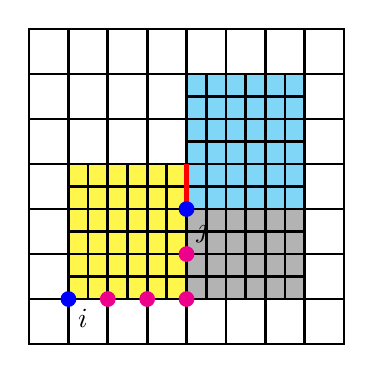
\begin{tikzpicture}[scale=4.0]
    % Define layers
    \pgfdeclarelayer{background}
    \pgfsetlayers{background,main}

    \coordinate (v1_1) at (0.0, 0.0);
    \coordinate (v1_2) at (0.125, 0.0);
    \coordinate (v1_3) at (0.125, 0.14285714285714285);
    \coordinate (v1_4) at (0.0, 0.14285714285714285);
    \draw[black, line width=1.0pt] (v1_1) -- (v1_2) -- (v1_3) -- (v1_4) -- cycle;
    \coordinate (v2_1) at (0.125, 0.0);
    \coordinate (v2_2) at (0.25, 0.0);
    \coordinate (v2_3) at (0.25, 0.14285714285714285);
    \coordinate (v2_4) at (0.125, 0.14285714285714285);
    \draw[black, line width=1.0pt] (v2_1) -- (v2_2) -- (v2_3) -- (v2_4) -- cycle;
    \coordinate (v3_1) at (0.25, 0.0);
    \coordinate (v3_2) at (0.375, 0.0);
    \coordinate (v3_3) at (0.375, 0.14285714285714285);
    \coordinate (v3_4) at (0.25, 0.14285714285714285);
    \draw[black, line width=1.0pt] (v3_1) -- (v3_2) -- (v3_3) -- (v3_4) -- cycle;
    \coordinate (v4_1) at (0.375, 0.0);
    \coordinate (v4_2) at (0.5, 0.0);
    \coordinate (v4_3) at (0.5, 0.14285714285714285);
    \coordinate (v4_4) at (0.375, 0.14285714285714285);
    \draw[black, line width=1.0pt] (v4_1) -- (v4_2) -- (v4_3) -- (v4_4) -- cycle;
    \coordinate (v5_1) at (0.5, 0.0);
    \coordinate (v5_2) at (0.625, 0.0);
    \coordinate (v5_3) at (0.625, 0.14285714285714285);
    \coordinate (v5_4) at (0.5, 0.14285714285714285);
    \draw[black, line width=1.0pt] (v5_1) -- (v5_2) -- (v5_3) -- (v5_4) -- cycle;
    \coordinate (v6_1) at (0.625, 0.0);
    \coordinate (v6_2) at (0.75, 0.0);
    \coordinate (v6_3) at (0.75, 0.14285714285714285);
    \coordinate (v6_4) at (0.625, 0.14285714285714285);
    \draw[black, line width=1.0pt] (v6_1) -- (v6_2) -- (v6_3) -- (v6_4) -- cycle;
    \coordinate (v7_1) at (0.75, 0.0);
    \coordinate (v7_2) at (0.875, 0.0);
    \coordinate (v7_3) at (0.875, 0.14285714285714285);
    \coordinate (v7_4) at (0.75, 0.14285714285714285);
    \draw[black, line width=1.0pt] (v7_1) -- (v7_2) -- (v7_3) -- (v7_4) -- cycle;
    \coordinate (v8_1) at (0.875, 0.0);
    \coordinate (v8_2) at (1.0, 0.0);
    \coordinate (v8_3) at (1.0, 0.14285714285714285);
    \coordinate (v8_4) at (0.875, 0.14285714285714285);
    \draw[black, line width=1.0pt] (v8_1) -- (v8_2) -- (v8_3) -- (v8_4) -- cycle;
    \coordinate (v9_1) at (0.0, 0.14285714285714285);
    \coordinate (v9_2) at (0.125, 0.14285714285714285);
    \coordinate (v9_3) at (0.125, 0.2857142857142857);
    \coordinate (v9_4) at (0.0, 0.2857142857142857);
    \draw[black, line width=1.0pt] (v9_1) -- (v9_2) -- (v9_3) -- (v9_4) -- cycle;
    \coordinate (v10_1) at (0.875, 0.14285714285714285);
    \coordinate (v10_2) at (1.0, 0.14285714285714285);
    \coordinate (v10_3) at (1.0, 0.2857142857142857);
    \coordinate (v10_4) at (0.875, 0.2857142857142857);
    \draw[black, line width=1.0pt] (v10_1) -- (v10_2) -- (v10_3) -- (v10_4) -- cycle;
    \coordinate (v11_1) at (0.0, 0.2857142857142857);
    \coordinate (v11_2) at (0.125, 0.2857142857142857);
    \coordinate (v11_3) at (0.125, 0.42857142857142855);
    \coordinate (v11_4) at (0.0, 0.42857142857142855);
    \draw[black, line width=1.0pt] (v11_1) -- (v11_2) -- (v11_3) -- (v11_4) -- cycle;
    \coordinate (v12_1) at (0.875, 0.2857142857142857);
    \coordinate (v12_2) at (1.0, 0.2857142857142857);
    \coordinate (v12_3) at (1.0, 0.42857142857142855);
    \coordinate (v12_4) at (0.875, 0.42857142857142855);
    \draw[black, line width=1.0pt] (v12_1) -- (v12_2) -- (v12_3) -- (v12_4) -- cycle;
    \coordinate (v13_1) at (0.0, 0.42857142857142855);
    \coordinate (v13_2) at (0.125, 0.42857142857142855);
    \coordinate (v13_3) at (0.125, 0.5714285714285714);
    \coordinate (v13_4) at (0.0, 0.5714285714285714);
    \draw[black, line width=1.0pt] (v13_1) -- (v13_2) -- (v13_3) -- (v13_4) -- cycle;
    \coordinate (v14_1) at (0.875, 0.42857142857142855);
    \coordinate (v14_2) at (1.0, 0.42857142857142855);
    \coordinate (v14_3) at (1.0, 0.5714285714285714);
    \coordinate (v14_4) at (0.875, 0.5714285714285714);
    \draw[black, line width=1.0pt] (v14_1) -- (v14_2) -- (v14_3) -- (v14_4) -- cycle;
    \coordinate (v15_1) at (0.0, 0.5714285714285714);
    \coordinate (v15_2) at (0.125, 0.5714285714285714);
    \coordinate (v15_3) at (0.125, 0.7142857142857143);
    \coordinate (v15_4) at (0.0, 0.7142857142857143);
    \draw[black, line width=1.0pt] (v15_1) -- (v15_2) -- (v15_3) -- (v15_4) -- cycle;
    \coordinate (v16_1) at (0.125, 0.5714285714285714);
    \coordinate (v16_2) at (0.25, 0.5714285714285714);
    \coordinate (v16_3) at (0.25, 0.7142857142857143);
    \coordinate (v16_4) at (0.125, 0.7142857142857143);
    \draw[black, line width=1.0pt] (v16_1) -- (v16_2) -- (v16_3) -- (v16_4) -- cycle;
    \coordinate (v17_1) at (0.25, 0.5714285714285714);
    \coordinate (v17_2) at (0.375, 0.5714285714285714);
    \coordinate (v17_3) at (0.375, 0.7142857142857143);
    \coordinate (v17_4) at (0.25, 0.7142857142857143);
    \draw[black, line width=1.0pt] (v17_1) -- (v17_2) -- (v17_3) -- (v17_4) -- cycle;
    \coordinate (v18_1) at (0.375, 0.5714285714285714);
    \coordinate (v18_2) at (0.5, 0.5714285714285714);
    \coordinate (v18_3) at (0.5, 0.7142857142857143);
    \coordinate (v18_4) at (0.375, 0.7142857142857143);
    \draw[black, line width=1.0pt] (v18_1) -- (v18_2) -- (v18_3) -- (v18_4) -- cycle;
    \coordinate (v19_1) at (0.875, 0.5714285714285714);
    \coordinate (v19_2) at (1.0, 0.5714285714285714);
    \coordinate (v19_3) at (1.0, 0.7142857142857143);
    \coordinate (v19_4) at (0.875, 0.7142857142857143);
    \draw[black, line width=1.0pt] (v19_1) -- (v19_2) -- (v19_3) -- (v19_4) -- cycle;
    \coordinate (v20_1) at (0.0, 0.7142857142857143);
    \coordinate (v20_2) at (0.125, 0.7142857142857143);
    \coordinate (v20_3) at (0.125, 0.8571428571428571);
    \coordinate (v20_4) at (0.0, 0.8571428571428571);
    \draw[black, line width=1.0pt] (v20_1) -- (v20_2) -- (v20_3) -- (v20_4) -- cycle;
    \coordinate (v21_1) at (0.125, 0.7142857142857143);
    \coordinate (v21_2) at (0.25, 0.7142857142857143);
    \coordinate (v21_3) at (0.25, 0.8571428571428571);
    \coordinate (v21_4) at (0.125, 0.8571428571428571);
    \draw[black, line width=1.0pt] (v21_1) -- (v21_2) -- (v21_3) -- (v21_4) -- cycle;
    \coordinate (v22_1) at (0.25, 0.7142857142857143);
    \coordinate (v22_2) at (0.375, 0.7142857142857143);
    \coordinate (v22_3) at (0.375, 0.8571428571428571);
    \coordinate (v22_4) at (0.25, 0.8571428571428571);
    \draw[black, line width=1.0pt] (v22_1) -- (v22_2) -- (v22_3) -- (v22_4) -- cycle;
    \coordinate (v23_1) at (0.375, 0.7142857142857143);
    \coordinate (v23_2) at (0.5, 0.7142857142857143);
    \coordinate (v23_3) at (0.5, 0.8571428571428571);
    \coordinate (v23_4) at (0.375, 0.8571428571428571);
    \draw[black, line width=1.0pt] (v23_1) -- (v23_2) -- (v23_3) -- (v23_4) -- cycle;
    \coordinate (v24_1) at (0.875, 0.7142857142857143);
    \coordinate (v24_2) at (1.0, 0.7142857142857143);
    \coordinate (v24_3) at (1.0, 0.8571428571428571);
    \coordinate (v24_4) at (0.875, 0.8571428571428571);
    \draw[black, line width=1.0pt] (v24_1) -- (v24_2) -- (v24_3) -- (v24_4) -- cycle;
    \coordinate (v25_1) at (0.0, 0.8571428571428571);
    \coordinate (v25_2) at (0.125, 0.8571428571428571);
    \coordinate (v25_3) at (0.125, 1.0);
    \coordinate (v25_4) at (0.0, 1.0);
    \draw[black, line width=1.0pt] (v25_1) -- (v25_2) -- (v25_3) -- (v25_4) -- cycle;
    \coordinate (v26_1) at (0.125, 0.8571428571428571);
    \coordinate (v26_2) at (0.25, 0.8571428571428571);
    \coordinate (v26_3) at (0.25, 1.0);
    \coordinate (v26_4) at (0.125, 1.0);
    \draw[black, line width=1.0pt] (v26_1) -- (v26_2) -- (v26_3) -- (v26_4) -- cycle;
    \coordinate (v27_1) at (0.25, 0.8571428571428571);
    \coordinate (v27_2) at (0.375, 0.8571428571428571);
    \coordinate (v27_3) at (0.375, 1.0);
    \coordinate (v27_4) at (0.25, 1.0);
    \draw[black, line width=1.0pt] (v27_1) -- (v27_2) -- (v27_3) -- (v27_4) -- cycle;
    \coordinate (v28_1) at (0.375, 0.8571428571428571);
    \coordinate (v28_2) at (0.5, 0.8571428571428571);
    \coordinate (v28_3) at (0.5, 1.0);
    \coordinate (v28_4) at (0.375, 1.0);
    \draw[black, line width=1.0pt] (v28_1) -- (v28_2) -- (v28_3) -- (v28_4) -- cycle;
    \coordinate (v29_1) at (0.5, 0.8571428571428571);
    \coordinate (v29_2) at (0.625, 0.8571428571428571);
    \coordinate (v29_3) at (0.625, 1.0);
    \coordinate (v29_4) at (0.5, 1.0);
    \draw[black, line width=1.0pt] (v29_1) -- (v29_2) -- (v29_3) -- (v29_4) -- cycle;
    \coordinate (v30_1) at (0.625, 0.8571428571428571);
    \coordinate (v30_2) at (0.75, 0.8571428571428571);
    \coordinate (v30_3) at (0.75, 1.0);
    \coordinate (v30_4) at (0.625, 1.0);
    \draw[black, line width=1.0pt] (v30_1) -- (v30_2) -- (v30_3) -- (v30_4) -- cycle;
    \coordinate (v31_1) at (0.75, 0.8571428571428571);
    \coordinate (v31_2) at (0.875, 0.8571428571428571);
    \coordinate (v31_3) at (0.875, 1.0);
    \coordinate (v31_4) at (0.75, 1.0);
    \draw[black, line width=1.0pt] (v31_1) -- (v31_2) -- (v31_3) -- (v31_4) -- cycle;
    \coordinate (v32_1) at (0.875, 0.8571428571428571);
    \coordinate (v32_2) at (1.0, 0.8571428571428571);
    \coordinate (v32_3) at (1.0, 1.0);
    \coordinate (v32_4) at (0.875, 1.0);
    \draw[black, line width=1.0pt] (v32_1) -- (v32_2) -- (v32_3) -- (v32_4) -- cycle;
    \coordinate (v33_1) at (0.125, 0.14285714285714285);
    \coordinate (v33_2) at (0.1875, 0.14285714285714285);
    \coordinate (v33_3) at (0.1875, 0.21428571428571427);
    \coordinate (v33_4) at (0.125, 0.21428571428571427);
    \draw[black, line width=1.0pt] (v33_1) -- (v33_2) -- (v33_3) -- (v33_4) -- cycle;
    \coordinate (v34_1) at (0.1875, 0.14285714285714285);
    \coordinate (v34_2) at (0.25, 0.14285714285714285);
    \coordinate (v34_3) at (0.25, 0.21428571428571427);
    \coordinate (v34_4) at (0.1875, 0.21428571428571427);
    \draw[black, line width=1.0pt] (v34_1) -- (v34_2) -- (v34_3) -- (v34_4) -- cycle;
    \coordinate (v35_1) at (0.25, 0.14285714285714285);
    \coordinate (v35_2) at (0.3125, 0.14285714285714285);
    \coordinate (v35_3) at (0.3125, 0.21428571428571427);
    \coordinate (v35_4) at (0.25, 0.21428571428571427);
    \draw[black, line width=1.0pt] (v35_1) -- (v35_2) -- (v35_3) -- (v35_4) -- cycle;
    \coordinate (v36_1) at (0.3125, 0.14285714285714285);
    \coordinate (v36_2) at (0.375, 0.14285714285714285);
    \coordinate (v36_3) at (0.375, 0.21428571428571427);
    \coordinate (v36_4) at (0.3125, 0.21428571428571427);
    \draw[black, line width=1.0pt] (v36_1) -- (v36_2) -- (v36_3) -- (v36_4) -- cycle;
    \coordinate (v37_1) at (0.375, 0.14285714285714285);
    \coordinate (v37_2) at (0.4375, 0.14285714285714285);
    \coordinate (v37_3) at (0.4375, 0.21428571428571427);
    \coordinate (v37_4) at (0.375, 0.21428571428571427);
    \draw[black, line width=1.0pt] (v37_1) -- (v37_2) -- (v37_3) -- (v37_4) -- cycle;
    \coordinate (v38_1) at (0.4375, 0.14285714285714285);
    \coordinate (v38_2) at (0.5, 0.14285714285714285);
    \coordinate (v38_3) at (0.5, 0.21428571428571427);
    \coordinate (v38_4) at (0.4375, 0.21428571428571427);
    \draw[black, line width=1.0pt] (v38_1) -- (v38_2) -- (v38_3) -- (v38_4) -- cycle;
    \coordinate (v39_1) at (0.5, 0.14285714285714285);
    \coordinate (v39_2) at (0.5625, 0.14285714285714285);
    \coordinate (v39_3) at (0.5625, 0.21428571428571427);
    \coordinate (v39_4) at (0.5, 0.21428571428571427);
    \draw[black, line width=1.0pt] (v39_1) -- (v39_2) -- (v39_3) -- (v39_4) -- cycle;
    \coordinate (v40_1) at (0.5625, 0.14285714285714285);
    \coordinate (v40_2) at (0.625, 0.14285714285714285);
    \coordinate (v40_3) at (0.625, 0.21428571428571427);
    \coordinate (v40_4) at (0.5625, 0.21428571428571427);
    \draw[black, line width=1.0pt] (v40_1) -- (v40_2) -- (v40_3) -- (v40_4) -- cycle;
    \coordinate (v41_1) at (0.625, 0.14285714285714285);
    \coordinate (v41_2) at (0.6875, 0.14285714285714285);
    \coordinate (v41_3) at (0.6875, 0.21428571428571427);
    \coordinate (v41_4) at (0.625, 0.21428571428571427);
    \draw[black, line width=1.0pt] (v41_1) -- (v41_2) -- (v41_3) -- (v41_4) -- cycle;
    \coordinate (v42_1) at (0.6875, 0.14285714285714285);
    \coordinate (v42_2) at (0.75, 0.14285714285714285);
    \coordinate (v42_3) at (0.75, 0.21428571428571427);
    \coordinate (v42_4) at (0.6875, 0.21428571428571427);
    \draw[black, line width=1.0pt] (v42_1) -- (v42_2) -- (v42_3) -- (v42_4) -- cycle;
    \coordinate (v43_1) at (0.75, 0.14285714285714285);
    \coordinate (v43_2) at (0.8125, 0.14285714285714285);
    \coordinate (v43_3) at (0.8125, 0.21428571428571427);
    \coordinate (v43_4) at (0.75, 0.21428571428571427);
    \draw[black, line width=1.0pt] (v43_1) -- (v43_2) -- (v43_3) -- (v43_4) -- cycle;
    \coordinate (v44_1) at (0.8125, 0.14285714285714285);
    \coordinate (v44_2) at (0.875, 0.14285714285714285);
    \coordinate (v44_3) at (0.875, 0.21428571428571427);
    \coordinate (v44_4) at (0.8125, 0.21428571428571427);
    \draw[black, line width=1.0pt] (v44_1) -- (v44_2) -- (v44_3) -- (v44_4) -- cycle;
    \coordinate (v45_1) at (0.125, 0.21428571428571427);
    \coordinate (v45_2) at (0.1875, 0.21428571428571427);
    \coordinate (v45_3) at (0.1875, 0.2857142857142857);
    \coordinate (v45_4) at (0.125, 0.2857142857142857);
    \draw[black, line width=1.0pt] (v45_1) -- (v45_2) -- (v45_3) -- (v45_4) -- cycle;
    \coordinate (v46_1) at (0.1875, 0.21428571428571427);
    \coordinate (v46_2) at (0.25, 0.21428571428571427);
    \coordinate (v46_3) at (0.25, 0.2857142857142857);
    \coordinate (v46_4) at (0.1875, 0.2857142857142857);
    \draw[black, line width=1.0pt] (v46_1) -- (v46_2) -- (v46_3) -- (v46_4) -- cycle;
    \coordinate (v47_1) at (0.25, 0.21428571428571427);
    \coordinate (v47_2) at (0.3125, 0.21428571428571427);
    \coordinate (v47_3) at (0.3125, 0.2857142857142857);
    \coordinate (v47_4) at (0.25, 0.2857142857142857);
    \draw[black, line width=1.0pt] (v47_1) -- (v47_2) -- (v47_3) -- (v47_4) -- cycle;
    \coordinate (v48_1) at (0.3125, 0.21428571428571427);
    \coordinate (v48_2) at (0.375, 0.21428571428571427);
    \coordinate (v48_3) at (0.375, 0.2857142857142857);
    \coordinate (v48_4) at (0.3125, 0.2857142857142857);
    \draw[black, line width=1.0pt] (v48_1) -- (v48_2) -- (v48_3) -- (v48_4) -- cycle;
    \coordinate (v49_1) at (0.375, 0.21428571428571427);
    \coordinate (v49_2) at (0.4375, 0.21428571428571427);
    \coordinate (v49_3) at (0.4375, 0.2857142857142857);
    \coordinate (v49_4) at (0.375, 0.2857142857142857);
    \draw[black, line width=1.0pt] (v49_1) -- (v49_2) -- (v49_3) -- (v49_4) -- cycle;
    \coordinate (v50_1) at (0.4375, 0.21428571428571427);
    \coordinate (v50_2) at (0.5, 0.21428571428571427);
    \coordinate (v50_3) at (0.5, 0.2857142857142857);
    \coordinate (v50_4) at (0.4375, 0.2857142857142857);
    \draw[black, line width=1.0pt] (v50_1) -- (v50_2) -- (v50_3) -- (v50_4) -- cycle;
    \coordinate (v51_1) at (0.5, 0.21428571428571427);
    \coordinate (v51_2) at (0.5625, 0.21428571428571427);
    \coordinate (v51_3) at (0.5625, 0.2857142857142857);
    \coordinate (v51_4) at (0.5, 0.2857142857142857);
    \draw[black, line width=1.0pt] (v51_1) -- (v51_2) -- (v51_3) -- (v51_4) -- cycle;
    \coordinate (v52_1) at (0.5625, 0.21428571428571427);
    \coordinate (v52_2) at (0.625, 0.21428571428571427);
    \coordinate (v52_3) at (0.625, 0.2857142857142857);
    \coordinate (v52_4) at (0.5625, 0.2857142857142857);
    \draw[black, line width=1.0pt] (v52_1) -- (v52_2) -- (v52_3) -- (v52_4) -- cycle;
    \coordinate (v53_1) at (0.625, 0.21428571428571427);
    \coordinate (v53_2) at (0.6875, 0.21428571428571427);
    \coordinate (v53_3) at (0.6875, 0.2857142857142857);
    \coordinate (v53_4) at (0.625, 0.2857142857142857);
    \draw[black, line width=1.0pt] (v53_1) -- (v53_2) -- (v53_3) -- (v53_4) -- cycle;
    \coordinate (v54_1) at (0.6875, 0.21428571428571427);
    \coordinate (v54_2) at (0.75, 0.21428571428571427);
    \coordinate (v54_3) at (0.75, 0.2857142857142857);
    \coordinate (v54_4) at (0.6875, 0.2857142857142857);
    \draw[black, line width=1.0pt] (v54_1) -- (v54_2) -- (v54_3) -- (v54_4) -- cycle;
    \coordinate (v55_1) at (0.75, 0.21428571428571427);
    \coordinate (v55_2) at (0.8125, 0.21428571428571427);
    \coordinate (v55_3) at (0.8125, 0.2857142857142857);
    \coordinate (v55_4) at (0.75, 0.2857142857142857);
    \draw[black, line width=1.0pt] (v55_1) -- (v55_2) -- (v55_3) -- (v55_4) -- cycle;
    \coordinate (v56_1) at (0.8125, 0.21428571428571427);
    \coordinate (v56_2) at (0.875, 0.21428571428571427);
    \coordinate (v56_3) at (0.875, 0.2857142857142857);
    \coordinate (v56_4) at (0.8125, 0.2857142857142857);
    \draw[black, line width=1.0pt] (v56_1) -- (v56_2) -- (v56_3) -- (v56_4) -- cycle;
    \coordinate (v57_1) at (0.125, 0.2857142857142857);
    \coordinate (v57_2) at (0.1875, 0.2857142857142857);
    \coordinate (v57_3) at (0.1875, 0.3571428571428571);
    \coordinate (v57_4) at (0.125, 0.3571428571428571);
    \draw[black, line width=1.0pt] (v57_1) -- (v57_2) -- (v57_3) -- (v57_4) -- cycle;
    \coordinate (v58_1) at (0.1875, 0.2857142857142857);
    \coordinate (v58_2) at (0.25, 0.2857142857142857);
    \coordinate (v58_3) at (0.25, 0.3571428571428571);
    \coordinate (v58_4) at (0.1875, 0.3571428571428571);
    \draw[black, line width=1.0pt] (v58_1) -- (v58_2) -- (v58_3) -- (v58_4) -- cycle;
    \coordinate (v59_1) at (0.25, 0.2857142857142857);
    \coordinate (v59_2) at (0.3125, 0.2857142857142857);
    \coordinate (v59_3) at (0.3125, 0.3571428571428571);
    \coordinate (v59_4) at (0.25, 0.3571428571428571);
    \draw[black, line width=1.0pt] (v59_1) -- (v59_2) -- (v59_3) -- (v59_4) -- cycle;
    \coordinate (v60_1) at (0.3125, 0.2857142857142857);
    \coordinate (v60_2) at (0.375, 0.2857142857142857);
    \coordinate (v60_3) at (0.375, 0.3571428571428571);
    \coordinate (v60_4) at (0.3125, 0.3571428571428571);
    \draw[black, line width=1.0pt] (v60_1) -- (v60_2) -- (v60_3) -- (v60_4) -- cycle;
    \coordinate (v61_1) at (0.375, 0.2857142857142857);
    \coordinate (v61_2) at (0.4375, 0.2857142857142857);
    \coordinate (v61_3) at (0.4375, 0.3571428571428571);
    \coordinate (v61_4) at (0.375, 0.3571428571428571);
    \draw[black, line width=1.0pt] (v61_1) -- (v61_2) -- (v61_3) -- (v61_4) -- cycle;
    \coordinate (v62_1) at (0.4375, 0.2857142857142857);
    \coordinate (v62_2) at (0.5, 0.2857142857142857);
    \coordinate (v62_3) at (0.5, 0.3571428571428571);
    \coordinate (v62_4) at (0.4375, 0.3571428571428571);
    \draw[black, line width=1.0pt] (v62_1) -- (v62_2) -- (v62_3) -- (v62_4) -- cycle;
    \coordinate (v63_1) at (0.5, 0.2857142857142857);
    \coordinate (v63_2) at (0.5625, 0.2857142857142857);
    \coordinate (v63_3) at (0.5625, 0.3571428571428571);
    \coordinate (v63_4) at (0.5, 0.3571428571428571);
    \draw[black, line width=1.0pt] (v63_1) -- (v63_2) -- (v63_3) -- (v63_4) -- cycle;
    \coordinate (v64_1) at (0.5625, 0.2857142857142857);
    \coordinate (v64_2) at (0.625, 0.2857142857142857);
    \coordinate (v64_3) at (0.625, 0.3571428571428571);
    \coordinate (v64_4) at (0.5625, 0.3571428571428571);
    \draw[black, line width=1.0pt] (v64_1) -- (v64_2) -- (v64_3) -- (v64_4) -- cycle;
    \coordinate (v65_1) at (0.625, 0.2857142857142857);
    \coordinate (v65_2) at (0.6875, 0.2857142857142857);
    \coordinate (v65_3) at (0.6875, 0.3571428571428571);
    \coordinate (v65_4) at (0.625, 0.3571428571428571);
    \draw[black, line width=1.0pt] (v65_1) -- (v65_2) -- (v65_3) -- (v65_4) -- cycle;
    \coordinate (v66_1) at (0.6875, 0.2857142857142857);
    \coordinate (v66_2) at (0.75, 0.2857142857142857);
    \coordinate (v66_3) at (0.75, 0.3571428571428571);
    \coordinate (v66_4) at (0.6875, 0.3571428571428571);
    \draw[black, line width=1.0pt] (v66_1) -- (v66_2) -- (v66_3) -- (v66_4) -- cycle;
    \coordinate (v67_1) at (0.75, 0.2857142857142857);
    \coordinate (v67_2) at (0.8125, 0.2857142857142857);
    \coordinate (v67_3) at (0.8125, 0.3571428571428571);
    \coordinate (v67_4) at (0.75, 0.3571428571428571);
    \draw[black, line width=1.0pt] (v67_1) -- (v67_2) -- (v67_3) -- (v67_4) -- cycle;
    \coordinate (v68_1) at (0.8125, 0.2857142857142857);
    \coordinate (v68_2) at (0.875, 0.2857142857142857);
    \coordinate (v68_3) at (0.875, 0.3571428571428571);
    \coordinate (v68_4) at (0.8125, 0.3571428571428571);
    \draw[black, line width=1.0pt] (v68_1) -- (v68_2) -- (v68_3) -- (v68_4) -- cycle;
    \coordinate (v69_1) at (0.125, 0.3571428571428571);
    \coordinate (v69_2) at (0.1875, 0.3571428571428571);
    \coordinate (v69_3) at (0.1875, 0.42857142857142855);
    \coordinate (v69_4) at (0.125, 0.42857142857142855);
    \draw[black, line width=1.0pt] (v69_1) -- (v69_2) -- (v69_3) -- (v69_4) -- cycle;
    \coordinate (v70_1) at (0.1875, 0.3571428571428571);
    \coordinate (v70_2) at (0.25, 0.3571428571428571);
    \coordinate (v70_3) at (0.25, 0.42857142857142855);
    \coordinate (v70_4) at (0.1875, 0.42857142857142855);
    \draw[black, line width=1.0pt] (v70_1) -- (v70_2) -- (v70_3) -- (v70_4) -- cycle;
    \coordinate (v71_1) at (0.25, 0.3571428571428571);
    \coordinate (v71_2) at (0.3125, 0.3571428571428571);
    \coordinate (v71_3) at (0.3125, 0.42857142857142855);
    \coordinate (v71_4) at (0.25, 0.42857142857142855);
    \draw[black, line width=1.0pt] (v71_1) -- (v71_2) -- (v71_3) -- (v71_4) -- cycle;
    \coordinate (v72_1) at (0.3125, 0.3571428571428571);
    \coordinate (v72_2) at (0.375, 0.3571428571428571);
    \coordinate (v72_3) at (0.375, 0.42857142857142855);
    \coordinate (v72_4) at (0.3125, 0.42857142857142855);
    \draw[black, line width=1.0pt] (v72_1) -- (v72_2) -- (v72_3) -- (v72_4) -- cycle;
    \coordinate (v73_1) at (0.375, 0.3571428571428571);
    \coordinate (v73_2) at (0.4375, 0.3571428571428571);
    \coordinate (v73_3) at (0.4375, 0.42857142857142855);
    \coordinate (v73_4) at (0.375, 0.42857142857142855);
    \draw[black, line width=1.0pt] (v73_1) -- (v73_2) -- (v73_3) -- (v73_4) -- cycle;
    \coordinate (v74_1) at (0.4375, 0.3571428571428571);
    \coordinate (v74_2) at (0.5, 0.3571428571428571);
    \coordinate (v74_3) at (0.5, 0.42857142857142855);
    \coordinate (v74_4) at (0.4375, 0.42857142857142855);
    \draw[black, line width=1.0pt] (v74_1) -- (v74_2) -- (v74_3) -- (v74_4) -- cycle;
    \coordinate (v75_1) at (0.5, 0.3571428571428571);
    \coordinate (v75_2) at (0.5625, 0.3571428571428571);
    \coordinate (v75_3) at (0.5625, 0.42857142857142855);
    \coordinate (v75_4) at (0.5, 0.42857142857142855);
    \draw[black, line width=1.0pt] (v75_1) -- (v75_2) -- (v75_3) -- (v75_4) -- cycle;
    \coordinate (v76_1) at (0.5625, 0.3571428571428571);
    \coordinate (v76_2) at (0.625, 0.3571428571428571);
    \coordinate (v76_3) at (0.625, 0.42857142857142855);
    \coordinate (v76_4) at (0.5625, 0.42857142857142855);
    \draw[black, line width=1.0pt] (v76_1) -- (v76_2) -- (v76_3) -- (v76_4) -- cycle;
    \coordinate (v77_1) at (0.625, 0.3571428571428571);
    \coordinate (v77_2) at (0.6875, 0.3571428571428571);
    \coordinate (v77_3) at (0.6875, 0.42857142857142855);
    \coordinate (v77_4) at (0.625, 0.42857142857142855);
    \draw[black, line width=1.0pt] (v77_1) -- (v77_2) -- (v77_3) -- (v77_4) -- cycle;
    \coordinate (v78_1) at (0.6875, 0.3571428571428571);
    \coordinate (v78_2) at (0.75, 0.3571428571428571);
    \coordinate (v78_3) at (0.75, 0.42857142857142855);
    \coordinate (v78_4) at (0.6875, 0.42857142857142855);
    \draw[black, line width=1.0pt] (v78_1) -- (v78_2) -- (v78_3) -- (v78_4) -- cycle;
    \coordinate (v79_1) at (0.75, 0.3571428571428571);
    \coordinate (v79_2) at (0.8125, 0.3571428571428571);
    \coordinate (v79_3) at (0.8125, 0.42857142857142855);
    \coordinate (v79_4) at (0.75, 0.42857142857142855);
    \draw[black, line width=1.0pt] (v79_1) -- (v79_2) -- (v79_3) -- (v79_4) -- cycle;
    \coordinate (v80_1) at (0.8125, 0.3571428571428571);
    \coordinate (v80_2) at (0.875, 0.3571428571428571);
    \coordinate (v80_3) at (0.875, 0.42857142857142855);
    \coordinate (v80_4) at (0.8125, 0.42857142857142855);
    \draw[black, line width=1.0pt] (v80_1) -- (v80_2) -- (v80_3) -- (v80_4) -- cycle;
    \coordinate (v81_1) at (0.125, 0.42857142857142855);
    \coordinate (v81_2) at (0.1875, 0.42857142857142855);
    \coordinate (v81_3) at (0.1875, 0.5);
    \coordinate (v81_4) at (0.125, 0.5);
    \draw[black, line width=1.0pt] (v81_1) -- (v81_2) -- (v81_3) -- (v81_4) -- cycle;
    \coordinate (v82_1) at (0.1875, 0.42857142857142855);
    \coordinate (v82_2) at (0.25, 0.42857142857142855);
    \coordinate (v82_3) at (0.25, 0.5);
    \coordinate (v82_4) at (0.1875, 0.5);
    \draw[black, line width=1.0pt] (v82_1) -- (v82_2) -- (v82_3) -- (v82_4) -- cycle;
    \coordinate (v83_1) at (0.25, 0.42857142857142855);
    \coordinate (v83_2) at (0.3125, 0.42857142857142855);
    \coordinate (v83_3) at (0.3125, 0.5);
    \coordinate (v83_4) at (0.25, 0.5);
    \draw[black, line width=1.0pt] (v83_1) -- (v83_2) -- (v83_3) -- (v83_4) -- cycle;
    \coordinate (v84_1) at (0.3125, 0.42857142857142855);
    \coordinate (v84_2) at (0.375, 0.42857142857142855);
    \coordinate (v84_3) at (0.375, 0.5);
    \coordinate (v84_4) at (0.3125, 0.5);
    \draw[black, line width=1.0pt] (v84_1) -- (v84_2) -- (v84_3) -- (v84_4) -- cycle;
    \coordinate (v85_1) at (0.375, 0.42857142857142855);
    \coordinate (v85_2) at (0.4375, 0.42857142857142855);
    \coordinate (v85_3) at (0.4375, 0.5);
    \coordinate (v85_4) at (0.375, 0.5);
    \draw[black, line width=1.0pt] (v85_1) -- (v85_2) -- (v85_3) -- (v85_4) -- cycle;
    \coordinate (v86_1) at (0.4375, 0.42857142857142855);
    \coordinate (v86_2) at (0.5, 0.42857142857142855);
    \coordinate (v86_3) at (0.5, 0.5);
    \coordinate (v86_4) at (0.4375, 0.5);
    \draw[black, line width=1.0pt] (v86_1) -- (v86_2) -- (v86_3) -- (v86_4) -- cycle;
    \coordinate (v87_1) at (0.5, 0.42857142857142855);
    \coordinate (v87_2) at (0.5625, 0.42857142857142855);
    \coordinate (v87_3) at (0.5625, 0.5);
    \coordinate (v87_4) at (0.5, 0.5);
    \draw[black, line width=1.0pt] (v87_1) -- (v87_2) -- (v87_3) -- (v87_4) -- cycle;
    \coordinate (v88_1) at (0.5625, 0.42857142857142855);
    \coordinate (v88_2) at (0.625, 0.42857142857142855);
    \coordinate (v88_3) at (0.625, 0.5);
    \coordinate (v88_4) at (0.5625, 0.5);
    \draw[black, line width=1.0pt] (v88_1) -- (v88_2) -- (v88_3) -- (v88_4) -- cycle;
    \coordinate (v89_1) at (0.625, 0.42857142857142855);
    \coordinate (v89_2) at (0.6875, 0.42857142857142855);
    \coordinate (v89_3) at (0.6875, 0.5);
    \coordinate (v89_4) at (0.625, 0.5);
    \draw[black, line width=1.0pt] (v89_1) -- (v89_2) -- (v89_3) -- (v89_4) -- cycle;
    \coordinate (v90_1) at (0.6875, 0.42857142857142855);
    \coordinate (v90_2) at (0.75, 0.42857142857142855);
    \coordinate (v90_3) at (0.75, 0.5);
    \coordinate (v90_4) at (0.6875, 0.5);
    \draw[black, line width=1.0pt] (v90_1) -- (v90_2) -- (v90_3) -- (v90_4) -- cycle;
    \coordinate (v91_1) at (0.75, 0.42857142857142855);
    \coordinate (v91_2) at (0.8125, 0.42857142857142855);
    \coordinate (v91_3) at (0.8125, 0.5);
    \coordinate (v91_4) at (0.75, 0.5);
    \draw[black, line width=1.0pt] (v91_1) -- (v91_2) -- (v91_3) -- (v91_4) -- cycle;
    \coordinate (v92_1) at (0.8125, 0.42857142857142855);
    \coordinate (v92_2) at (0.875, 0.42857142857142855);
    \coordinate (v92_3) at (0.875, 0.5);
    \coordinate (v92_4) at (0.8125, 0.5);
    \draw[black, line width=1.0pt] (v92_1) -- (v92_2) -- (v92_3) -- (v92_4) -- cycle;
    \coordinate (v93_1) at (0.125, 0.5);
    \coordinate (v93_2) at (0.1875, 0.5);
    \coordinate (v93_3) at (0.1875, 0.5714285714285714);
    \coordinate (v93_4) at (0.125, 0.5714285714285714);
    \draw[black, line width=1.0pt] (v93_1) -- (v93_2) -- (v93_3) -- (v93_4) -- cycle;
    \coordinate (v94_1) at (0.1875, 0.5);
    \coordinate (v94_2) at (0.25, 0.5);
    \coordinate (v94_3) at (0.25, 0.5714285714285714);
    \coordinate (v94_4) at (0.1875, 0.5714285714285714);
    \draw[black, line width=1.0pt] (v94_1) -- (v94_2) -- (v94_3) -- (v94_4) -- cycle;
    \coordinate (v95_1) at (0.25, 0.5);
    \coordinate (v95_2) at (0.3125, 0.5);
    \coordinate (v95_3) at (0.3125, 0.5714285714285714);
    \coordinate (v95_4) at (0.25, 0.5714285714285714);
    \draw[black, line width=1.0pt] (v95_1) -- (v95_2) -- (v95_3) -- (v95_4) -- cycle;
    \coordinate (v96_1) at (0.3125, 0.5);
    \coordinate (v96_2) at (0.375, 0.5);
    \coordinate (v96_3) at (0.375, 0.5714285714285714);
    \coordinate (v96_4) at (0.3125, 0.5714285714285714);
    \draw[black, line width=1.0pt] (v96_1) -- (v96_2) -- (v96_3) -- (v96_4) -- cycle;
    \coordinate (v97_1) at (0.375, 0.5);
    \coordinate (v97_2) at (0.4375, 0.5);
    \coordinate (v97_3) at (0.4375, 0.5714285714285714);
    \coordinate (v97_4) at (0.375, 0.5714285714285714);
    \draw[black, line width=1.0pt] (v97_1) -- (v97_2) -- (v97_3) -- (v97_4) -- cycle;
    \coordinate (v98_1) at (0.4375, 0.5);
    \coordinate (v98_2) at (0.5, 0.5);
    \coordinate (v98_3) at (0.5, 0.5714285714285714);
    \coordinate (v98_4) at (0.4375, 0.5714285714285714);
    \draw[black, line width=1.0pt] (v98_1) -- (v98_2) -- (v98_3) -- (v98_4) -- cycle;
    \coordinate (v99_1) at (0.5, 0.5);
    \coordinate (v99_2) at (0.5625, 0.5);
    \coordinate (v99_3) at (0.5625, 0.5714285714285714);
    \coordinate (v99_4) at (0.5, 0.5714285714285714);
    \draw[black, line width=1.0pt] (v99_1) -- (v99_2) -- (v99_3) -- (v99_4) -- cycle;
    \coordinate (v100_1) at (0.5625, 0.5);
    \coordinate (v100_2) at (0.625, 0.5);
    \coordinate (v100_3) at (0.625, 0.5714285714285714);
    \coordinate (v100_4) at (0.5625, 0.5714285714285714);
    \draw[black, line width=1.0pt] (v100_1) -- (v100_2) -- (v100_3) -- (v100_4) -- cycle;
    \coordinate (v101_1) at (0.625, 0.5);
    \coordinate (v101_2) at (0.6875, 0.5);
    \coordinate (v101_3) at (0.6875, 0.5714285714285714);
    \coordinate (v101_4) at (0.625, 0.5714285714285714);
    \draw[black, line width=1.0pt] (v101_1) -- (v101_2) -- (v101_3) -- (v101_4) -- cycle;
    \coordinate (v102_1) at (0.6875, 0.5);
    \coordinate (v102_2) at (0.75, 0.5);
    \coordinate (v102_3) at (0.75, 0.5714285714285714);
    \coordinate (v102_4) at (0.6875, 0.5714285714285714);
    \draw[black, line width=1.0pt] (v102_1) -- (v102_2) -- (v102_3) -- (v102_4) -- cycle;
    \coordinate (v103_1) at (0.75, 0.5);
    \coordinate (v103_2) at (0.8125, 0.5);
    \coordinate (v103_3) at (0.8125, 0.5714285714285714);
    \coordinate (v103_4) at (0.75, 0.5714285714285714);
    \draw[black, line width=1.0pt] (v103_1) -- (v103_2) -- (v103_3) -- (v103_4) -- cycle;
    \coordinate (v104_1) at (0.8125, 0.5);
    \coordinate (v104_2) at (0.875, 0.5);
    \coordinate (v104_3) at (0.875, 0.5714285714285714);
    \coordinate (v104_4) at (0.8125, 0.5714285714285714);
    \draw[black, line width=1.0pt] (v104_1) -- (v104_2) -- (v104_3) -- (v104_4) -- cycle;
    \coordinate (v105_1) at (0.5, 0.5714285714285714);
    \coordinate (v105_2) at (0.5625, 0.5714285714285714);
    \coordinate (v105_3) at (0.5625, 0.6428571428571428);
    \coordinate (v105_4) at (0.5, 0.6428571428571428);
    \draw[black, line width=1.0pt] (v105_1) -- (v105_2) -- (v105_3) -- (v105_4) -- cycle;
    \coordinate (v106_1) at (0.5625, 0.5714285714285714);
    \coordinate (v106_2) at (0.625, 0.5714285714285714);
    \coordinate (v106_3) at (0.625, 0.6428571428571428);
    \coordinate (v106_4) at (0.5625, 0.6428571428571428);
    \draw[black, line width=1.0pt] (v106_1) -- (v106_2) -- (v106_3) -- (v106_4) -- cycle;
    \coordinate (v107_1) at (0.625, 0.5714285714285714);
    \coordinate (v107_2) at (0.6875, 0.5714285714285714);
    \coordinate (v107_3) at (0.6875, 0.6428571428571428);
    \coordinate (v107_4) at (0.625, 0.6428571428571428);
    \draw[black, line width=1.0pt] (v107_1) -- (v107_2) -- (v107_3) -- (v107_4) -- cycle;
    \coordinate (v108_1) at (0.6875, 0.5714285714285714);
    \coordinate (v108_2) at (0.75, 0.5714285714285714);
    \coordinate (v108_3) at (0.75, 0.6428571428571428);
    \coordinate (v108_4) at (0.6875, 0.6428571428571428);
    \draw[black, line width=1.0pt] (v108_1) -- (v108_2) -- (v108_3) -- (v108_4) -- cycle;
    \coordinate (v109_1) at (0.75, 0.5714285714285714);
    \coordinate (v109_2) at (0.8125, 0.5714285714285714);
    \coordinate (v109_3) at (0.8125, 0.6428571428571428);
    \coordinate (v109_4) at (0.75, 0.6428571428571428);
    \draw[black, line width=1.0pt] (v109_1) -- (v109_2) -- (v109_3) -- (v109_4) -- cycle;
    \coordinate (v110_1) at (0.8125, 0.5714285714285714);
    \coordinate (v110_2) at (0.875, 0.5714285714285714);
    \coordinate (v110_3) at (0.875, 0.6428571428571428);
    \coordinate (v110_4) at (0.8125, 0.6428571428571428);
    \draw[black, line width=1.0pt] (v110_1) -- (v110_2) -- (v110_3) -- (v110_4) -- cycle;
    \coordinate (v111_1) at (0.5, 0.6428571428571428);
    \coordinate (v111_2) at (0.5625, 0.6428571428571428);
    \coordinate (v111_3) at (0.5625, 0.7142857142857143);
    \coordinate (v111_4) at (0.5, 0.7142857142857143);
    \draw[black, line width=1.0pt] (v111_1) -- (v111_2) -- (v111_3) -- (v111_4) -- cycle;
    \coordinate (v112_1) at (0.5625, 0.6428571428571428);
    \coordinate (v112_2) at (0.625, 0.6428571428571428);
    \coordinate (v112_3) at (0.625, 0.7142857142857143);
    \coordinate (v112_4) at (0.5625, 0.7142857142857143);
    \draw[black, line width=1.0pt] (v112_1) -- (v112_2) -- (v112_3) -- (v112_4) -- cycle;
    \coordinate (v113_1) at (0.625, 0.6428571428571428);
    \coordinate (v113_2) at (0.6875, 0.6428571428571428);
    \coordinate (v113_3) at (0.6875, 0.7142857142857143);
    \coordinate (v113_4) at (0.625, 0.7142857142857143);
    \draw[black, line width=1.0pt] (v113_1) -- (v113_2) -- (v113_3) -- (v113_4) -- cycle;
    \coordinate (v114_1) at (0.6875, 0.6428571428571428);
    \coordinate (v114_2) at (0.75, 0.6428571428571428);
    \coordinate (v114_3) at (0.75, 0.7142857142857143);
    \coordinate (v114_4) at (0.6875, 0.7142857142857143);
    \draw[black, line width=1.0pt] (v114_1) -- (v114_2) -- (v114_3) -- (v114_4) -- cycle;
    \coordinate (v115_1) at (0.75, 0.6428571428571428);
    \coordinate (v115_2) at (0.8125, 0.6428571428571428);
    \coordinate (v115_3) at (0.8125, 0.7142857142857143);
    \coordinate (v115_4) at (0.75, 0.7142857142857143);
    \draw[black, line width=1.0pt] (v115_1) -- (v115_2) -- (v115_3) -- (v115_4) -- cycle;
    \coordinate (v116_1) at (0.8125, 0.6428571428571428);
    \coordinate (v116_2) at (0.875, 0.6428571428571428);
    \coordinate (v116_3) at (0.875, 0.7142857142857143);
    \coordinate (v116_4) at (0.8125, 0.7142857142857143);
    \draw[black, line width=1.0pt] (v116_1) -- (v116_2) -- (v116_3) -- (v116_4) -- cycle;
    \coordinate (v117_1) at (0.5, 0.7142857142857143);
    \coordinate (v117_2) at (0.5625, 0.7142857142857143);
    \coordinate (v117_3) at (0.5625, 0.7857142857142857);
    \coordinate (v117_4) at (0.5, 0.7857142857142857);
    \draw[black, line width=1.0pt] (v117_1) -- (v117_2) -- (v117_3) -- (v117_4) -- cycle;
    \coordinate (v118_1) at (0.5625, 0.7142857142857143);
    \coordinate (v118_2) at (0.625, 0.7142857142857143);
    \coordinate (v118_3) at (0.625, 0.7857142857142857);
    \coordinate (v118_4) at (0.5625, 0.7857142857142857);
    \draw[black, line width=1.0pt] (v118_1) -- (v118_2) -- (v118_3) -- (v118_4) -- cycle;
    \coordinate (v119_1) at (0.625, 0.7142857142857143);
    \coordinate (v119_2) at (0.6875, 0.7142857142857143);
    \coordinate (v119_3) at (0.6875, 0.7857142857142857);
    \coordinate (v119_4) at (0.625, 0.7857142857142857);
    \draw[black, line width=1.0pt] (v119_1) -- (v119_2) -- (v119_3) -- (v119_4) -- cycle;
    \coordinate (v120_1) at (0.6875, 0.7142857142857143);
    \coordinate (v120_2) at (0.75, 0.7142857142857143);
    \coordinate (v120_3) at (0.75, 0.7857142857142857);
    \coordinate (v120_4) at (0.6875, 0.7857142857142857);
    \draw[black, line width=1.0pt] (v120_1) -- (v120_2) -- (v120_3) -- (v120_4) -- cycle;
    \coordinate (v121_1) at (0.75, 0.7142857142857143);
    \coordinate (v121_2) at (0.8125, 0.7142857142857143);
    \coordinate (v121_3) at (0.8125, 0.7857142857142857);
    \coordinate (v121_4) at (0.75, 0.7857142857142857);
    \draw[black, line width=1.0pt] (v121_1) -- (v121_2) -- (v121_3) -- (v121_4) -- cycle;
    \coordinate (v122_1) at (0.8125, 0.7142857142857143);
    \coordinate (v122_2) at (0.875, 0.7142857142857143);
    \coordinate (v122_3) at (0.875, 0.7857142857142857);
    \coordinate (v122_4) at (0.8125, 0.7857142857142857);
    \draw[black, line width=1.0pt] (v122_1) -- (v122_2) -- (v122_3) -- (v122_4) -- cycle;
    \coordinate (v123_1) at (0.5, 0.7857142857142857);
    \coordinate (v123_2) at (0.5625, 0.7857142857142857);
    \coordinate (v123_3) at (0.5625, 0.8571428571428571);
    \coordinate (v123_4) at (0.5, 0.8571428571428571);
    \draw[black, line width=1.0pt] (v123_1) -- (v123_2) -- (v123_3) -- (v123_4) -- cycle;
    \coordinate (v124_1) at (0.5625, 0.7857142857142857);
    \coordinate (v124_2) at (0.625, 0.7857142857142857);
    \coordinate (v124_3) at (0.625, 0.8571428571428571);
    \coordinate (v124_4) at (0.5625, 0.8571428571428571);
    \draw[black, line width=1.0pt] (v124_1) -- (v124_2) -- (v124_3) -- (v124_4) -- cycle;
    \coordinate (v125_1) at (0.625, 0.7857142857142857);
    \coordinate (v125_2) at (0.6875, 0.7857142857142857);
    \coordinate (v125_3) at (0.6875, 0.8571428571428571);
    \coordinate (v125_4) at (0.625, 0.8571428571428571);
    \draw[black, line width=1.0pt] (v125_1) -- (v125_2) -- (v125_3) -- (v125_4) -- cycle;
    \coordinate (v126_1) at (0.6875, 0.7857142857142857);
    \coordinate (v126_2) at (0.75, 0.7857142857142857);
    \coordinate (v126_3) at (0.75, 0.8571428571428571);
    \coordinate (v126_4) at (0.6875, 0.8571428571428571);
    \draw[black, line width=1.0pt] (v126_1) -- (v126_2) -- (v126_3) -- (v126_4) -- cycle;
    \coordinate (v127_1) at (0.75, 0.7857142857142857);
    \coordinate (v127_2) at (0.8125, 0.7857142857142857);
    \coordinate (v127_3) at (0.8125, 0.8571428571428571);
    \coordinate (v127_4) at (0.75, 0.8571428571428571);
    \draw[black, line width=1.0pt] (v127_1) -- (v127_2) -- (v127_3) -- (v127_4) -- cycle;
    \coordinate (v128_1) at (0.8125, 0.7857142857142857);
    \coordinate (v128_2) at (0.875, 0.7857142857142857);
    \coordinate (v128_3) at (0.875, 0.8571428571428571);
    \coordinate (v128_4) at (0.8125, 0.8571428571428571);
    \draw[black, line width=1.0pt] (v128_1) -- (v128_2) -- (v128_3) -- (v128_4) -- cycle;

     % Fill the pair support
    \begin{pgfonlayer}{background}
        \fill[gray, opacity=0.6] (v5_4) rectangle (v12_4);
        \fill[yellow, opacity=0.7] (v9_2) rectangle (v18_2);
        \fill[cyan, opacity=0.5] (v75_4) rectangle (v128_3);
    \end{pgfonlayer}

    \draw[red, line width=1.5] (v75_4) -- (v105_1);

    \node[anchor=north west] at (v9_2) {\(\boldvec{i}\)};
    \node[anchor=north west] at (v75_4) {\(\boldvec{j}\)};
    
    \fill[magenta] (v3_4) circle (0.025);
    \fill[magenta] (v4_4) circle (0.025);
    \fill[magenta] (v5_4) circle (0.025);
    \fill[magenta] (v63_1) circle (0.025);
    %\draw[magenta, line width=1.0pt] (v9_2) -- (v3_4) --  (v54_1) -- (v9_3) -- cycle;
    \fill[blue] (v9_2) circle (0.025);
    \fill[blue] (v75_4) circle (0.025);

\end{tikzpicture}

        \caption{}
        \label{fig:problematic-pair-algorithm-case-3-illustration}
    \end{subfigure}
    \hfill
    \strut
    \caption{
		Illustration of \Cref{alg:nlintersec,alg:shortest-chain} for three different cases,
		all using \(p_{(\level, k)} = 2\) for all \(\level\) and \(k\). In the left figure
		there is no problematic pair, in the centre figure there is a problematic pair and
		in the last figure there is a \nlintersec and a shortest chain, so the pair is not
		problematic. The union of all shaded cells represents \(\domain_{\level+1}\), while
		the supports of \(\xbsp_{\boldvec{i}}\) and
		\(\xbsp_{\boldvec{j}}\) are coloured in yellow and cyan,
		respectively, and their intersection in green. Also, the possible \(I_k\) contained
		in the intersection of the supports of \(\xbsp_{\boldvec{i}}\)
		and \(\xbsp_{\boldvec{j}}\), as in \Cref{def:nlintersec}, are
		highlighted in red.
		Finally, blue dots represent the indices \(\boldvec{i}\) and \(\boldvec{j}\) and
		magenta dots the indices of the other B-splines in \(\Bll\).
    }
    \label{fig:problematic-pair-algorithm-illustration}
\end{figure}

\begin{lem}
    \Cref{alg:exact-mesh} always produces an exact mesh.
\end{lem}
\begin{proof}
	The result follows as a consequence of
	\cref{lem:L-chain-shortest,lem:problematic-sides,lem:problematic-chain}.
\end{proof}


\section{Experiments}
\label{sec:experiments}
The experiments are designed to address two key research questions.
First, \textbf{RQ1} evaluates whether the average $L_2$-norm of the counterfactual perturbation vectors ($\overline{||\perturb||}$) decreases as the model overfits the data, thereby providing further empirical validation for our hypothesis.
Second, \textbf{RQ2} evaluates the ability of the proposed counterfactual regularized loss, as defined in (\ref{eq:regularized_loss2}), to mitigate overfitting when compared to existing regularization techniques.

% The experiments are designed to address three key research questions. First, \textbf{RQ1} investigates whether the mean perturbation vector norm decreases as the model overfits the data, aiming to further validate our intuition. Second, \textbf{RQ2} explores whether the mean perturbation vector norm can be effectively leveraged as a regularization term during training, offering insights into its potential role in mitigating overfitting. Finally, \textbf{RQ3} examines whether our counterfactual regularizer enables the model to achieve superior performance compared to existing regularization methods, thus highlighting its practical advantage.

\subsection{Experimental Setup}
\textbf{\textit{Datasets, Models, and Tasks.}}
The experiments are conducted on three datasets: \textit{Water Potability}~\cite{kadiwal2020waterpotability}, \textit{Phomene}~\cite{phomene}, and \textit{CIFAR-10}~\cite{krizhevsky2009learning}. For \textit{Water Potability} and \textit{Phomene}, we randomly select $80\%$ of the samples for the training set, and the remaining $20\%$ for the test set, \textit{CIFAR-10} comes already split. Furthermore, we consider the following models: Logistic Regression, Multi-Layer Perceptron (MLP) with 100 and 30 neurons on each hidden layer, and PreactResNet-18~\cite{he2016cvecvv} as a Convolutional Neural Network (CNN) architecture.
We focus on binary classification tasks and leave the extension to multiclass scenarios for future work. However, for datasets that are inherently multiclass, we transform the problem into a binary classification task by selecting two classes, aligning with our assumption.

\smallskip
\noindent\textbf{\textit{Evaluation Measures.}} To characterize the degree of overfitting, we use the test loss, as it serves as a reliable indicator of the model's generalization capability to unseen data. Additionally, we evaluate the predictive performance of each model using the test accuracy.

\smallskip
\noindent\textbf{\textit{Baselines.}} We compare CF-Reg with the following regularization techniques: L1 (``Lasso''), L2 (``Ridge''), and Dropout.

\smallskip
\noindent\textbf{\textit{Configurations.}}
For each model, we adopt specific configurations as follows.
\begin{itemize}
\item \textit{Logistic Regression:} To induce overfitting in the model, we artificially increase the dimensionality of the data beyond the number of training samples by applying a polynomial feature expansion. This approach ensures that the model has enough capacity to overfit the training data, allowing us to analyze the impact of our counterfactual regularizer. The degree of the polynomial is chosen as the smallest degree that makes the number of features greater than the number of data.
\item \textit{Neural Networks (MLP and CNN):} To take advantage of the closed-form solution for computing the optimal perturbation vector as defined in (\ref{eq:opt-delta}), we use a local linear approximation of the neural network models. Hence, given an instance $\inst_i$, we consider the (optimal) counterfactual not with respect to $\model$ but with respect to:
\begin{equation}
\label{eq:taylor}
    \model^{lin}(\inst) = \model(\inst_i) + \nabla_{\inst}\model(\inst_i)(\inst - \inst_i),
\end{equation}
where $\model^{lin}$ represents the first-order Taylor approximation of $\model$ at $\inst_i$.
Note that this step is unnecessary for Logistic Regression, as it is inherently a linear model.
\end{itemize}

\smallskip
\noindent \textbf{\textit{Implementation Details.}} We run all experiments on a machine equipped with an AMD Ryzen 9 7900 12-Core Processor and an NVIDIA GeForce RTX 4090 GPU. Our implementation is based on the PyTorch Lightning framework. We use stochastic gradient descent as the optimizer with a learning rate of $\eta = 0.001$ and no weight decay. We use a batch size of $128$. The training and test steps are conducted for $6000$ epochs on the \textit{Water Potability} and \textit{Phoneme} datasets, while for the \textit{CIFAR-10} dataset, they are performed for $200$ epochs.
Finally, the contribution $w_i^{\varepsilon}$ of each training point $\inst_i$ is uniformly set as $w_i^{\varepsilon} = 1~\forall i\in \{1,\ldots,m\}$.

The source code implementation for our experiments is available at the following GitHub repository: \url{https://anonymous.4open.science/r/COCE-80B4/README.md} 

\subsection{RQ1: Counterfactual Perturbation vs. Overfitting}
To address \textbf{RQ1}, we analyze the relationship between the test loss and the average $L_2$-norm of the counterfactual perturbation vectors ($\overline{||\perturb||}$) over training epochs.

In particular, Figure~\ref{fig:delta_loss_epochs} depicts the evolution of $\overline{||\perturb||}$ alongside the test loss for an MLP trained \textit{without} regularization on the \textit{Water Potability} dataset. 
\begin{figure}[ht]
    \centering
    \includegraphics[width=0.85\linewidth]{img/delta_loss_epochs.png}
    \caption{The average counterfactual perturbation vector $\overline{||\perturb||}$ (left $y$-axis) and the cross-entropy test loss (right $y$-axis) over training epochs ($x$-axis) for an MLP trained on the \textit{Water Potability} dataset \textit{without} regularization.}
    \label{fig:delta_loss_epochs}
\end{figure}

The plot shows a clear trend as the model starts to overfit the data (evidenced by an increase in test loss). 
Notably, $\overline{||\perturb||}$ begins to decrease, which aligns with the hypothesis that the average distance to the optimal counterfactual example gets smaller as the model's decision boundary becomes increasingly adherent to the training data.

It is worth noting that this trend is heavily influenced by the choice of the counterfactual generator model. In particular, the relationship between $\overline{||\perturb||}$ and the degree of overfitting may become even more pronounced when leveraging more accurate counterfactual generators. However, these models often come at the cost of higher computational complexity, and their exploration is left to future work.

Nonetheless, we expect that $\overline{||\perturb||}$ will eventually stabilize at a plateau, as the average $L_2$-norm of the optimal counterfactual perturbations cannot vanish to zero.

% Additionally, the choice of employing the score-based counterfactual explanation framework to generate counterfactuals was driven to promote computational efficiency.

% Future enhancements to the framework may involve adopting models capable of generating more precise counterfactuals. While such approaches may yield to performance improvements, they are likely to come at the cost of increased computational complexity.


\subsection{RQ2: Counterfactual Regularization Performance}
To answer \textbf{RQ2}, we evaluate the effectiveness of the proposed counterfactual regularization (CF-Reg) by comparing its performance against existing baselines: unregularized training loss (No-Reg), L1 regularization (L1-Reg), L2 regularization (L2-Reg), and Dropout.
Specifically, for each model and dataset combination, Table~\ref{tab:regularization_comparison} presents the mean value and standard deviation of test accuracy achieved by each method across 5 random initialization. 

The table illustrates that our regularization technique consistently delivers better results than existing methods across all evaluated scenarios, except for one case -- i.e., Logistic Regression on the \textit{Phomene} dataset. 
However, this setting exhibits an unusual pattern, as the highest model accuracy is achieved without any regularization. Even in this case, CF-Reg still surpasses other regularization baselines.

From the results above, we derive the following key insights. First, CF-Reg proves to be effective across various model types, ranging from simple linear models (Logistic Regression) to deep architectures like MLPs and CNNs, and across diverse datasets, including both tabular and image data. 
Second, CF-Reg's strong performance on the \textit{Water} dataset with Logistic Regression suggests that its benefits may be more pronounced when applied to simpler models. However, the unexpected outcome on the \textit{Phoneme} dataset calls for further investigation into this phenomenon.


\begin{table*}[h!]
    \centering
    \caption{Mean value and standard deviation of test accuracy across 5 random initializations for different model, dataset, and regularization method. The best results are highlighted in \textbf{bold}.}
    \label{tab:regularization_comparison}
    \begin{tabular}{|c|c|c|c|c|c|c|}
        \hline
        \textbf{Model} & \textbf{Dataset} & \textbf{No-Reg} & \textbf{L1-Reg} & \textbf{L2-Reg} & \textbf{Dropout} & \textbf{CF-Reg (ours)} \\ \hline
        Logistic Regression   & \textit{Water}   & $0.6595 \pm 0.0038$   & $0.6729 \pm 0.0056$   & $0.6756 \pm 0.0046$  & N/A    & $\mathbf{0.6918 \pm 0.0036}$                     \\ \hline
        MLP   & \textit{Water}   & $0.6756 \pm 0.0042$   & $0.6790 \pm 0.0058$   & $0.6790 \pm 0.0023$  & $0.6750 \pm 0.0036$    & $\mathbf{0.6802 \pm 0.0046}$                    \\ \hline
%        MLP   & \textit{Adult}   & $0.8404 \pm 0.0010$   & $\mathbf{0.8495 \pm 0.0007}$   & $0.8489 \pm 0.0014$  & $\mathbf{0.8495 \pm 0.0016}$     & $0.8449 \pm 0.0019$                    \\ \hline
        Logistic Regression   & \textit{Phomene}   & $\mathbf{0.8148 \pm 0.0020}$   & $0.8041 \pm 0.0028$   & $0.7835 \pm 0.0176$  & N/A    & $0.8098 \pm 0.0055$                     \\ \hline
        MLP   & \textit{Phomene}   & $0.8677 \pm 0.0033$   & $0.8374 \pm 0.0080$   & $0.8673 \pm 0.0045$  & $0.8672 \pm 0.0042$     & $\mathbf{0.8718 \pm 0.0040}$                    \\ \hline
        CNN   & \textit{CIFAR-10} & $0.6670 \pm 0.0233$   & $0.6229 \pm 0.0850$   & $0.7348 \pm 0.0365$   & N/A    & $\mathbf{0.7427 \pm 0.0571}$                     \\ \hline
    \end{tabular}
\end{table*}

\begin{table*}[htb!]
    \centering
    \caption{Hyperparameter configurations utilized for the generation of Table \ref{tab:regularization_comparison}. For our regularization the hyperparameters are reported as $\mathbf{\alpha/\beta}$.}
    \label{tab:performance_parameters}
    \begin{tabular}{|c|c|c|c|c|c|c|}
        \hline
        \textbf{Model} & \textbf{Dataset} & \textbf{No-Reg} & \textbf{L1-Reg} & \textbf{L2-Reg} & \textbf{Dropout} & \textbf{CF-Reg (ours)} \\ \hline
        Logistic Regression   & \textit{Water}   & N/A   & $0.0093$   & $0.6927$  & N/A    & $0.3791/1.0355$                     \\ \hline
        MLP   & \textit{Water}   & N/A   & $0.0007$   & $0.0022$  & $0.0002$    & $0.2567/1.9775$                    \\ \hline
        Logistic Regression   &
        \textit{Phomene}   & N/A   & $0.0097$   & $0.7979$  & N/A    & $0.0571/1.8516$                     \\ \hline
        MLP   & \textit{Phomene}   & N/A   & $0.0007$   & $4.24\cdot10^{-5}$  & $0.0015$    & $0.0516/2.2700$                    \\ \hline
       % MLP   & \textit{Adult}   & N/A   & $0.0018$   & $0.0018$  & $0.0601$     & $0.0764/2.2068$                    \\ \hline
        CNN   & \textit{CIFAR-10} & N/A   & $0.0050$   & $0.0864$ & N/A    & $0.3018/
        2.1502$                     \\ \hline
    \end{tabular}
\end{table*}

\begin{table*}[htb!]
    \centering
    \caption{Mean value and standard deviation of training time across 5 different runs. The reported time (in seconds) corresponds to the generation of each entry in Table \ref{tab:regularization_comparison}. Times are }
    \label{tab:times}
    \begin{tabular}{|c|c|c|c|c|c|c|}
        \hline
        \textbf{Model} & \textbf{Dataset} & \textbf{No-Reg} & \textbf{L1-Reg} & \textbf{L2-Reg} & \textbf{Dropout} & \textbf{CF-Reg (ours)} \\ \hline
        Logistic Regression   & \textit{Water}   & $222.98 \pm 1.07$   & $239.94 \pm 2.59$   & $241.60 \pm 1.88$  & N/A    & $251.50 \pm 1.93$                     \\ \hline
        MLP   & \textit{Water}   & $225.71 \pm 3.85$   & $250.13 \pm 4.44$   & $255.78 \pm 2.38$  & $237.83 \pm 3.45$    & $266.48 \pm 3.46$                    \\ \hline
        Logistic Regression   & \textit{Phomene}   & $266.39 \pm 0.82$ & $367.52 \pm 6.85$   & $361.69 \pm 4.04$  & N/A   & $310.48 \pm 0.76$                    \\ \hline
        MLP   &
        \textit{Phomene} & $335.62 \pm 1.77$   & $390.86 \pm 2.11$   & $393.96 \pm 1.95$ & $363.51 \pm 5.07$    & $403.14 \pm 1.92$                     \\ \hline
       % MLP   & \textit{Adult}   & N/A   & $0.0018$   & $0.0018$  & $0.0601$     & $0.0764/2.2068$                    \\ \hline
        CNN   & \textit{CIFAR-10} & $370.09 \pm 0.18$   & $395.71 \pm 0.55$   & $401.38 \pm 0.16$ & N/A    & $1287.8 \pm 0.26$                     \\ \hline
    \end{tabular}
\end{table*}

\subsection{Feasibility of our Method}
A crucial requirement for any regularization technique is that it should impose minimal impact on the overall training process.
In this respect, CF-Reg introduces an overhead that depends on the time required to find the optimal counterfactual example for each training instance. 
As such, the more sophisticated the counterfactual generator model probed during training the higher would be the time required. However, a more advanced counterfactual generator might provide a more effective regularization. We discuss this trade-off in more details in Section~\ref{sec:discussion}.

Table~\ref{tab:times} presents the average training time ($\pm$ standard deviation) for each model and dataset combination listed in Table~\ref{tab:regularization_comparison}.
We can observe that the higher accuracy achieved by CF-Reg using the score-based counterfactual generator comes with only minimal overhead. However, when applied to deep neural networks with many hidden layers, such as \textit{PreactResNet-18}, the forward derivative computation required for the linearization of the network introduces a more noticeable computational cost, explaining the longer training times in the table.

\subsection{Hyperparameter Sensitivity Analysis}
The proposed counterfactual regularization technique relies on two key hyperparameters: $\alpha$ and $\beta$. The former is intrinsic to the loss formulation defined in (\ref{eq:cf-train}), while the latter is closely tied to the choice of the score-based counterfactual explanation method used.

Figure~\ref{fig:test_alpha_beta} illustrates how the test accuracy of an MLP trained on the \textit{Water Potability} dataset changes for different combinations of $\alpha$ and $\beta$.

\begin{figure}[ht]
    \centering
    \includegraphics[width=0.85\linewidth]{img/test_acc_alpha_beta.png}
    \caption{The test accuracy of an MLP trained on the \textit{Water Potability} dataset, evaluated while varying the weight of our counterfactual regularizer ($\alpha$) for different values of $\beta$.}
    \label{fig:test_alpha_beta}
\end{figure}

We observe that, for a fixed $\beta$, increasing the weight of our counterfactual regularizer ($\alpha$) can slightly improve test accuracy until a sudden drop is noticed for $\alpha > 0.1$.
This behavior was expected, as the impact of our penalty, like any regularization term, can be disruptive if not properly controlled.

Moreover, this finding further demonstrates that our regularization method, CF-Reg, is inherently data-driven. Therefore, it requires specific fine-tuning based on the combination of the model and dataset at hand.

\section{Conclusion}

We present a set of algorithms for range retrieval on high-dimensional datasets using graph-based indices. To improve the performance of queries with no range results, we introduce an early stopping mechanism capable of significantly decreasing the time taken to terminate searches on such queries. We also introduce two extensions of beam search, greedy search and doubling search, for efficient range queries with hundreds to tens of thousands of results. Combined, our techniques achieved up to 100x speedup over a naive baseline, with 5-10x speedup in almost all cases. We introduce a benchmark of nine datasets, including datasets with up to 100 million points, and demonstrate strong performance and scalability for our algorithms on these datasets. 

Our results yield significant improvement over the naive baseline, and established a wide-ranging benchmark for performance. As we tackle a relatively unexplored problem, many areas for further improvement are still available. One natural extension would be to explore more sophisticated metrics for our early stopping algorithm, perhaps using machine learning methods, as better early termination of queries with few results has potential for significant impact on overall search times. Another would be to explore extensions of the range retrieval benchmark itself; for example, Szilvasy et al.~\cite{szilvasy2024vector} argue that the range search benchmark should differentiate between results which are very close to the query point and points which are close to the radius boundary, giving the former more weight. In preliminary experiments, we attempted to use a simple weighting mechanism based on a point's distance to the query point when calculating precision, but we were unable to find a weighting that changed the precision values significantly. However, future work identifying such mechanisms would be very practical and promising.

{
%% Acknowledgments
\begin{acks}                            %% acks environment is optional
	%% contents suppressed with 'anonymous'
	
	This work was supported in part by the National Science Foundation
	grants CCF-2119352 and CCF-1919223. 
\end{acks}
}

\clearpage
%% Bibliography
\bibliography{../bibliography/strings,../bibliography/main}


%%% Appendix
\unless\ifx\fullversion\undefined

\subsection{Lloyd-Max Algorithm}
\label{subsec:Lloyd-Max}
For a given quantization bitwidth $B$ and an operand $\bm{X}$, the Lloyd-Max algorithm finds $2^B$ quantization levels $\{\hat{x}_i\}_{i=1}^{2^B}$ such that quantizing $\bm{X}$ by rounding each scalar in $\bm{X}$ to the nearest quantization level minimizes the quantization MSE. 

The algorithm starts with an initial guess of quantization levels and then iteratively computes quantization thresholds $\{\tau_i\}_{i=1}^{2^B-1}$ and updates quantization levels $\{\hat{x}_i\}_{i=1}^{2^B}$. Specifically, at iteration $n$, thresholds are set to the midpoints of the previous iteration's levels:
\begin{align*}
    \tau_i^{(n)}=\frac{\hat{x}_i^{(n-1)}+\hat{x}_{i+1}^{(n-1)}}2 \text{ for } i=1\ldots 2^B-1
\end{align*}
Subsequently, the quantization levels are re-computed as conditional means of the data regions defined by the new thresholds:
\begin{align*}
    \hat{x}_i^{(n)}=\mathbb{E}\left[ \bm{X} \big| \bm{X}\in [\tau_{i-1}^{(n)},\tau_i^{(n)}] \right] \text{ for } i=1\ldots 2^B
\end{align*}
where to satisfy boundary conditions we have $\tau_0=-\infty$ and $\tau_{2^B}=\infty$. The algorithm iterates the above steps until convergence.

Figure \ref{fig:lm_quant} compares the quantization levels of a $7$-bit floating point (E3M3) quantizer (left) to a $7$-bit Lloyd-Max quantizer (right) when quantizing a layer of weights from the GPT3-126M model at a per-tensor granularity. As shown, the Lloyd-Max quantizer achieves substantially lower quantization MSE. Further, Table \ref{tab:FP7_vs_LM7} shows the superior perplexity achieved by Lloyd-Max quantizers for bitwidths of $7$, $6$ and $5$. The difference between the quantizers is clear at 5 bits, where per-tensor FP quantization incurs a drastic and unacceptable increase in perplexity, while Lloyd-Max quantization incurs a much smaller increase. Nevertheless, we note that even the optimal Lloyd-Max quantizer incurs a notable ($\sim 1.5$) increase in perplexity due to the coarse granularity of quantization. 

\begin{figure}[h]
  \centering
  \includegraphics[width=0.7\linewidth]{sections/figures/LM7_FP7.pdf}
  \caption{\small Quantization levels and the corresponding quantization MSE of Floating Point (left) vs Lloyd-Max (right) Quantizers for a layer of weights in the GPT3-126M model.}
  \label{fig:lm_quant}
\end{figure}

\begin{table}[h]\scriptsize
\begin{center}
\caption{\label{tab:FP7_vs_LM7} \small Comparing perplexity (lower is better) achieved by floating point quantizers and Lloyd-Max quantizers on a GPT3-126M model for the Wikitext-103 dataset.}
\begin{tabular}{c|cc|c}
\hline
 \multirow{2}{*}{\textbf{Bitwidth}} & \multicolumn{2}{|c|}{\textbf{Floating-Point Quantizer}} & \textbf{Lloyd-Max Quantizer} \\
 & Best Format & Wikitext-103 Perplexity & Wikitext-103 Perplexity \\
\hline
7 & E3M3 & 18.32 & 18.27 \\
6 & E3M2 & 19.07 & 18.51 \\
5 & E4M0 & 43.89 & 19.71 \\
\hline
\end{tabular}
\end{center}
\end{table}

\subsection{Proof of Local Optimality of LO-BCQ}
\label{subsec:lobcq_opt_proof}
For a given block $\bm{b}_j$, the quantization MSE during LO-BCQ can be empirically evaluated as $\frac{1}{L_b}\lVert \bm{b}_j- \bm{\hat{b}}_j\rVert^2_2$ where $\bm{\hat{b}}_j$ is computed from equation (\ref{eq:clustered_quantization_definition}) as $C_{f(\bm{b}_j)}(\bm{b}_j)$. Further, for a given block cluster $\mathcal{B}_i$, we compute the quantization MSE as $\frac{1}{|\mathcal{B}_{i}|}\sum_{\bm{b} \in \mathcal{B}_{i}} \frac{1}{L_b}\lVert \bm{b}- C_i^{(n)}(\bm{b})\rVert^2_2$. Therefore, at the end of iteration $n$, we evaluate the overall quantization MSE $J^{(n)}$ for a given operand $\bm{X}$ composed of $N_c$ block clusters as:
\begin{align*}
    \label{eq:mse_iter_n}
    J^{(n)} = \frac{1}{N_c} \sum_{i=1}^{N_c} \frac{1}{|\mathcal{B}_{i}^{(n)}|}\sum_{\bm{v} \in \mathcal{B}_{i}^{(n)}} \frac{1}{L_b}\lVert \bm{b}- B_i^{(n)}(\bm{b})\rVert^2_2
\end{align*}

At the end of iteration $n$, the codebooks are updated from $\mathcal{C}^{(n-1)}$ to $\mathcal{C}^{(n)}$. However, the mapping of a given vector $\bm{b}_j$ to quantizers $\mathcal{C}^{(n)}$ remains as  $f^{(n)}(\bm{b}_j)$. At the next iteration, during the vector clustering step, $f^{(n+1)}(\bm{b}_j)$ finds new mapping of $\bm{b}_j$ to updated codebooks $\mathcal{C}^{(n)}$ such that the quantization MSE over the candidate codebooks is minimized. Therefore, we obtain the following result for $\bm{b}_j$:
\begin{align*}
\frac{1}{L_b}\lVert \bm{b}_j - C_{f^{(n+1)}(\bm{b}_j)}^{(n)}(\bm{b}_j)\rVert^2_2 \le \frac{1}{L_b}\lVert \bm{b}_j - C_{f^{(n)}(\bm{b}_j)}^{(n)}(\bm{b}_j)\rVert^2_2
\end{align*}

That is, quantizing $\bm{b}_j$ at the end of the block clustering step of iteration $n+1$ results in lower quantization MSE compared to quantizing at the end of iteration $n$. Since this is true for all $\bm{b} \in \bm{X}$, we assert the following:
\begin{equation}
\begin{split}
\label{eq:mse_ineq_1}
    \tilde{J}^{(n+1)} &= \frac{1}{N_c} \sum_{i=1}^{N_c} \frac{1}{|\mathcal{B}_{i}^{(n+1)}|}\sum_{\bm{b} \in \mathcal{B}_{i}^{(n+1)}} \frac{1}{L_b}\lVert \bm{b} - C_i^{(n)}(b)\rVert^2_2 \le J^{(n)}
\end{split}
\end{equation}
where $\tilde{J}^{(n+1)}$ is the the quantization MSE after the vector clustering step at iteration $n+1$.

Next, during the codebook update step (\ref{eq:quantizers_update}) at iteration $n+1$, the per-cluster codebooks $\mathcal{C}^{(n)}$ are updated to $\mathcal{C}^{(n+1)}$ by invoking the Lloyd-Max algorithm \citep{Lloyd}. We know that for any given value distribution, the Lloyd-Max algorithm minimizes the quantization MSE. Therefore, for a given vector cluster $\mathcal{B}_i$ we obtain the following result:

\begin{equation}
    \frac{1}{|\mathcal{B}_{i}^{(n+1)}|}\sum_{\bm{b} \in \mathcal{B}_{i}^{(n+1)}} \frac{1}{L_b}\lVert \bm{b}- C_i^{(n+1)}(\bm{b})\rVert^2_2 \le \frac{1}{|\mathcal{B}_{i}^{(n+1)}|}\sum_{\bm{b} \in \mathcal{B}_{i}^{(n+1)}} \frac{1}{L_b}\lVert \bm{b}- C_i^{(n)}(\bm{b})\rVert^2_2
\end{equation}

The above equation states that quantizing the given block cluster $\mathcal{B}_i$ after updating the associated codebook from $C_i^{(n)}$ to $C_i^{(n+1)}$ results in lower quantization MSE. Since this is true for all the block clusters, we derive the following result: 
\begin{equation}
\begin{split}
\label{eq:mse_ineq_2}
     J^{(n+1)} &= \frac{1}{N_c} \sum_{i=1}^{N_c} \frac{1}{|\mathcal{B}_{i}^{(n+1)}|}\sum_{\bm{b} \in \mathcal{B}_{i}^{(n+1)}} \frac{1}{L_b}\lVert \bm{b}- C_i^{(n+1)}(\bm{b})\rVert^2_2  \le \tilde{J}^{(n+1)}   
\end{split}
\end{equation}

Following (\ref{eq:mse_ineq_1}) and (\ref{eq:mse_ineq_2}), we find that the quantization MSE is non-increasing for each iteration, that is, $J^{(1)} \ge J^{(2)} \ge J^{(3)} \ge \ldots \ge J^{(M)}$ where $M$ is the maximum number of iterations. 
%Therefore, we can say that if the algorithm converges, then it must be that it has converged to a local minimum. 
\hfill $\blacksquare$


\begin{figure}
    \begin{center}
    \includegraphics[width=0.5\textwidth]{sections//figures/mse_vs_iter.pdf}
    \end{center}
    \caption{\small NMSE vs iterations during LO-BCQ compared to other block quantization proposals}
    \label{fig:nmse_vs_iter}
\end{figure}

Figure \ref{fig:nmse_vs_iter} shows the empirical convergence of LO-BCQ across several block lengths and number of codebooks. Also, the MSE achieved by LO-BCQ is compared to baselines such as MXFP and VSQ. As shown, LO-BCQ converges to a lower MSE than the baselines. Further, we achieve better convergence for larger number of codebooks ($N_c$) and for a smaller block length ($L_b$), both of which increase the bitwidth of BCQ (see Eq \ref{eq:bitwidth_bcq}).


\subsection{Additional Accuracy Results}
%Table \ref{tab:lobcq_config} lists the various LOBCQ configurations and their corresponding bitwidths.
\begin{table}
\setlength{\tabcolsep}{4.75pt}
\begin{center}
\caption{\label{tab:lobcq_config} Various LO-BCQ configurations and their bitwidths.}
\begin{tabular}{|c||c|c|c|c||c|c||c|} 
\hline
 & \multicolumn{4}{|c||}{$L_b=8$} & \multicolumn{2}{|c||}{$L_b=4$} & $L_b=2$ \\
 \hline
 \backslashbox{$L_A$\kern-1em}{\kern-1em$N_c$} & 2 & 4 & 8 & 16 & 2 & 4 & 2 \\
 \hline
 64 & 4.25 & 4.375 & 4.5 & 4.625 & 4.375 & 4.625 & 4.625\\
 \hline
 32 & 4.375 & 4.5 & 4.625& 4.75 & 4.5 & 4.75 & 4.75 \\
 \hline
 16 & 4.625 & 4.75& 4.875 & 5 & 4.75 & 5 & 5 \\
 \hline
\end{tabular}
\end{center}
\end{table}

%\subsection{Perplexity achieved by various LO-BCQ configurations on Wikitext-103 dataset}

\begin{table} \centering
\begin{tabular}{|c||c|c|c|c||c|c||c|} 
\hline
 $L_b \rightarrow$& \multicolumn{4}{c||}{8} & \multicolumn{2}{c||}{4} & 2\\
 \hline
 \backslashbox{$L_A$\kern-1em}{\kern-1em$N_c$} & 2 & 4 & 8 & 16 & 2 & 4 & 2  \\
 %$N_c \rightarrow$ & 2 & 4 & 8 & 16 & 2 & 4 & 2 \\
 \hline
 \hline
 \multicolumn{8}{c}{GPT3-1.3B (FP32 PPL = 9.98)} \\ 
 \hline
 \hline
 64 & 10.40 & 10.23 & 10.17 & 10.15 &  10.28 & 10.18 & 10.19 \\
 \hline
 32 & 10.25 & 10.20 & 10.15 & 10.12 &  10.23 & 10.17 & 10.17 \\
 \hline
 16 & 10.22 & 10.16 & 10.10 & 10.09 &  10.21 & 10.14 & 10.16 \\
 \hline
  \hline
 \multicolumn{8}{c}{GPT3-8B (FP32 PPL = 7.38)} \\ 
 \hline
 \hline
 64 & 7.61 & 7.52 & 7.48 &  7.47 &  7.55 &  7.49 & 7.50 \\
 \hline
 32 & 7.52 & 7.50 & 7.46 &  7.45 &  7.52 &  7.48 & 7.48  \\
 \hline
 16 & 7.51 & 7.48 & 7.44 &  7.44 &  7.51 &  7.49 & 7.47  \\
 \hline
\end{tabular}
\caption{\label{tab:ppl_gpt3_abalation} Wikitext-103 perplexity across GPT3-1.3B and 8B models.}
\end{table}

\begin{table} \centering
\begin{tabular}{|c||c|c|c|c||} 
\hline
 $L_b \rightarrow$& \multicolumn{4}{c||}{8}\\
 \hline
 \backslashbox{$L_A$\kern-1em}{\kern-1em$N_c$} & 2 & 4 & 8 & 16 \\
 %$N_c \rightarrow$ & 2 & 4 & 8 & 16 & 2 & 4 & 2 \\
 \hline
 \hline
 \multicolumn{5}{|c|}{Llama2-7B (FP32 PPL = 5.06)} \\ 
 \hline
 \hline
 64 & 5.31 & 5.26 & 5.19 & 5.18  \\
 \hline
 32 & 5.23 & 5.25 & 5.18 & 5.15  \\
 \hline
 16 & 5.23 & 5.19 & 5.16 & 5.14  \\
 \hline
 \multicolumn{5}{|c|}{Nemotron4-15B (FP32 PPL = 5.87)} \\ 
 \hline
 \hline
 64  & 6.3 & 6.20 & 6.13 & 6.08  \\
 \hline
 32  & 6.24 & 6.12 & 6.07 & 6.03  \\
 \hline
 16  & 6.12 & 6.14 & 6.04 & 6.02  \\
 \hline
 \multicolumn{5}{|c|}{Nemotron4-340B (FP32 PPL = 3.48)} \\ 
 \hline
 \hline
 64 & 3.67 & 3.62 & 3.60 & 3.59 \\
 \hline
 32 & 3.63 & 3.61 & 3.59 & 3.56 \\
 \hline
 16 & 3.61 & 3.58 & 3.57 & 3.55 \\
 \hline
\end{tabular}
\caption{\label{tab:ppl_llama7B_nemo15B} Wikitext-103 perplexity compared to FP32 baseline in Llama2-7B and Nemotron4-15B, 340B models}
\end{table}

%\subsection{Perplexity achieved by various LO-BCQ configurations on MMLU dataset}


\begin{table} \centering
\begin{tabular}{|c||c|c|c|c||c|c|c|c|} 
\hline
 $L_b \rightarrow$& \multicolumn{4}{c||}{8} & \multicolumn{4}{c||}{8}\\
 \hline
 \backslashbox{$L_A$\kern-1em}{\kern-1em$N_c$} & 2 & 4 & 8 & 16 & 2 & 4 & 8 & 16  \\
 %$N_c \rightarrow$ & 2 & 4 & 8 & 16 & 2 & 4 & 2 \\
 \hline
 \hline
 \multicolumn{5}{|c|}{Llama2-7B (FP32 Accuracy = 45.8\%)} & \multicolumn{4}{|c|}{Llama2-70B (FP32 Accuracy = 69.12\%)} \\ 
 \hline
 \hline
 64 & 43.9 & 43.4 & 43.9 & 44.9 & 68.07 & 68.27 & 68.17 & 68.75 \\
 \hline
 32 & 44.5 & 43.8 & 44.9 & 44.5 & 68.37 & 68.51 & 68.35 & 68.27  \\
 \hline
 16 & 43.9 & 42.7 & 44.9 & 45 & 68.12 & 68.77 & 68.31 & 68.59  \\
 \hline
 \hline
 \multicolumn{5}{|c|}{GPT3-22B (FP32 Accuracy = 38.75\%)} & \multicolumn{4}{|c|}{Nemotron4-15B (FP32 Accuracy = 64.3\%)} \\ 
 \hline
 \hline
 64 & 36.71 & 38.85 & 38.13 & 38.92 & 63.17 & 62.36 & 63.72 & 64.09 \\
 \hline
 32 & 37.95 & 38.69 & 39.45 & 38.34 & 64.05 & 62.30 & 63.8 & 64.33  \\
 \hline
 16 & 38.88 & 38.80 & 38.31 & 38.92 & 63.22 & 63.51 & 63.93 & 64.43  \\
 \hline
\end{tabular}
\caption{\label{tab:mmlu_abalation} Accuracy on MMLU dataset across GPT3-22B, Llama2-7B, 70B and Nemotron4-15B models.}
\end{table}


%\subsection{Perplexity achieved by various LO-BCQ configurations on LM evaluation harness}

\begin{table} \centering
\begin{tabular}{|c||c|c|c|c||c|c|c|c|} 
\hline
 $L_b \rightarrow$& \multicolumn{4}{c||}{8} & \multicolumn{4}{c||}{8}\\
 \hline
 \backslashbox{$L_A$\kern-1em}{\kern-1em$N_c$} & 2 & 4 & 8 & 16 & 2 & 4 & 8 & 16  \\
 %$N_c \rightarrow$ & 2 & 4 & 8 & 16 & 2 & 4 & 2 \\
 \hline
 \hline
 \multicolumn{5}{|c|}{Race (FP32 Accuracy = 37.51\%)} & \multicolumn{4}{|c|}{Boolq (FP32 Accuracy = 64.62\%)} \\ 
 \hline
 \hline
 64 & 36.94 & 37.13 & 36.27 & 37.13 & 63.73 & 62.26 & 63.49 & 63.36 \\
 \hline
 32 & 37.03 & 36.36 & 36.08 & 37.03 & 62.54 & 63.51 & 63.49 & 63.55  \\
 \hline
 16 & 37.03 & 37.03 & 36.46 & 37.03 & 61.1 & 63.79 & 63.58 & 63.33  \\
 \hline
 \hline
 \multicolumn{5}{|c|}{Winogrande (FP32 Accuracy = 58.01\%)} & \multicolumn{4}{|c|}{Piqa (FP32 Accuracy = 74.21\%)} \\ 
 \hline
 \hline
 64 & 58.17 & 57.22 & 57.85 & 58.33 & 73.01 & 73.07 & 73.07 & 72.80 \\
 \hline
 32 & 59.12 & 58.09 & 57.85 & 58.41 & 73.01 & 73.94 & 72.74 & 73.18  \\
 \hline
 16 & 57.93 & 58.88 & 57.93 & 58.56 & 73.94 & 72.80 & 73.01 & 73.94  \\
 \hline
\end{tabular}
\caption{\label{tab:mmlu_abalation} Accuracy on LM evaluation harness tasks on GPT3-1.3B model.}
\end{table}

\begin{table} \centering
\begin{tabular}{|c||c|c|c|c||c|c|c|c|} 
\hline
 $L_b \rightarrow$& \multicolumn{4}{c||}{8} & \multicolumn{4}{c||}{8}\\
 \hline
 \backslashbox{$L_A$\kern-1em}{\kern-1em$N_c$} & 2 & 4 & 8 & 16 & 2 & 4 & 8 & 16  \\
 %$N_c \rightarrow$ & 2 & 4 & 8 & 16 & 2 & 4 & 2 \\
 \hline
 \hline
 \multicolumn{5}{|c|}{Race (FP32 Accuracy = 41.34\%)} & \multicolumn{4}{|c|}{Boolq (FP32 Accuracy = 68.32\%)} \\ 
 \hline
 \hline
 64 & 40.48 & 40.10 & 39.43 & 39.90 & 69.20 & 68.41 & 69.45 & 68.56 \\
 \hline
 32 & 39.52 & 39.52 & 40.77 & 39.62 & 68.32 & 67.43 & 68.17 & 69.30  \\
 \hline
 16 & 39.81 & 39.71 & 39.90 & 40.38 & 68.10 & 66.33 & 69.51 & 69.42  \\
 \hline
 \hline
 \multicolumn{5}{|c|}{Winogrande (FP32 Accuracy = 67.88\%)} & \multicolumn{4}{|c|}{Piqa (FP32 Accuracy = 78.78\%)} \\ 
 \hline
 \hline
 64 & 66.85 & 66.61 & 67.72 & 67.88 & 77.31 & 77.42 & 77.75 & 77.64 \\
 \hline
 32 & 67.25 & 67.72 & 67.72 & 67.00 & 77.31 & 77.04 & 77.80 & 77.37  \\
 \hline
 16 & 68.11 & 68.90 & 67.88 & 67.48 & 77.37 & 78.13 & 78.13 & 77.69  \\
 \hline
\end{tabular}
\caption{\label{tab:mmlu_abalation} Accuracy on LM evaluation harness tasks on GPT3-8B model.}
\end{table}

\begin{table} \centering
\begin{tabular}{|c||c|c|c|c||c|c|c|c|} 
\hline
 $L_b \rightarrow$& \multicolumn{4}{c||}{8} & \multicolumn{4}{c||}{8}\\
 \hline
 \backslashbox{$L_A$\kern-1em}{\kern-1em$N_c$} & 2 & 4 & 8 & 16 & 2 & 4 & 8 & 16  \\
 %$N_c \rightarrow$ & 2 & 4 & 8 & 16 & 2 & 4 & 2 \\
 \hline
 \hline
 \multicolumn{5}{|c|}{Race (FP32 Accuracy = 40.67\%)} & \multicolumn{4}{|c|}{Boolq (FP32 Accuracy = 76.54\%)} \\ 
 \hline
 \hline
 64 & 40.48 & 40.10 & 39.43 & 39.90 & 75.41 & 75.11 & 77.09 & 75.66 \\
 \hline
 32 & 39.52 & 39.52 & 40.77 & 39.62 & 76.02 & 76.02 & 75.96 & 75.35  \\
 \hline
 16 & 39.81 & 39.71 & 39.90 & 40.38 & 75.05 & 73.82 & 75.72 & 76.09  \\
 \hline
 \hline
 \multicolumn{5}{|c|}{Winogrande (FP32 Accuracy = 70.64\%)} & \multicolumn{4}{|c|}{Piqa (FP32 Accuracy = 79.16\%)} \\ 
 \hline
 \hline
 64 & 69.14 & 70.17 & 70.17 & 70.56 & 78.24 & 79.00 & 78.62 & 78.73 \\
 \hline
 32 & 70.96 & 69.69 & 71.27 & 69.30 & 78.56 & 79.49 & 79.16 & 78.89  \\
 \hline
 16 & 71.03 & 69.53 & 69.69 & 70.40 & 78.13 & 79.16 & 79.00 & 79.00  \\
 \hline
\end{tabular}
\caption{\label{tab:mmlu_abalation} Accuracy on LM evaluation harness tasks on GPT3-22B model.}
\end{table}

\begin{table} \centering
\begin{tabular}{|c||c|c|c|c||c|c|c|c|} 
\hline
 $L_b \rightarrow$& \multicolumn{4}{c||}{8} & \multicolumn{4}{c||}{8}\\
 \hline
 \backslashbox{$L_A$\kern-1em}{\kern-1em$N_c$} & 2 & 4 & 8 & 16 & 2 & 4 & 8 & 16  \\
 %$N_c \rightarrow$ & 2 & 4 & 8 & 16 & 2 & 4 & 2 \\
 \hline
 \hline
 \multicolumn{5}{|c|}{Race (FP32 Accuracy = 44.4\%)} & \multicolumn{4}{|c|}{Boolq (FP32 Accuracy = 79.29\%)} \\ 
 \hline
 \hline
 64 & 42.49 & 42.51 & 42.58 & 43.45 & 77.58 & 77.37 & 77.43 & 78.1 \\
 \hline
 32 & 43.35 & 42.49 & 43.64 & 43.73 & 77.86 & 75.32 & 77.28 & 77.86  \\
 \hline
 16 & 44.21 & 44.21 & 43.64 & 42.97 & 78.65 & 77 & 76.94 & 77.98  \\
 \hline
 \hline
 \multicolumn{5}{|c|}{Winogrande (FP32 Accuracy = 69.38\%)} & \multicolumn{4}{|c|}{Piqa (FP32 Accuracy = 78.07\%)} \\ 
 \hline
 \hline
 64 & 68.9 & 68.43 & 69.77 & 68.19 & 77.09 & 76.82 & 77.09 & 77.86 \\
 \hline
 32 & 69.38 & 68.51 & 68.82 & 68.90 & 78.07 & 76.71 & 78.07 & 77.86  \\
 \hline
 16 & 69.53 & 67.09 & 69.38 & 68.90 & 77.37 & 77.8 & 77.91 & 77.69  \\
 \hline
\end{tabular}
\caption{\label{tab:mmlu_abalation} Accuracy on LM evaluation harness tasks on Llama2-7B model.}
\end{table}

\begin{table} \centering
\begin{tabular}{|c||c|c|c|c||c|c|c|c|} 
\hline
 $L_b \rightarrow$& \multicolumn{4}{c||}{8} & \multicolumn{4}{c||}{8}\\
 \hline
 \backslashbox{$L_A$\kern-1em}{\kern-1em$N_c$} & 2 & 4 & 8 & 16 & 2 & 4 & 8 & 16  \\
 %$N_c \rightarrow$ & 2 & 4 & 8 & 16 & 2 & 4 & 2 \\
 \hline
 \hline
 \multicolumn{5}{|c|}{Race (FP32 Accuracy = 48.8\%)} & \multicolumn{4}{|c|}{Boolq (FP32 Accuracy = 85.23\%)} \\ 
 \hline
 \hline
 64 & 49.00 & 49.00 & 49.28 & 48.71 & 82.82 & 84.28 & 84.03 & 84.25 \\
 \hline
 32 & 49.57 & 48.52 & 48.33 & 49.28 & 83.85 & 84.46 & 84.31 & 84.93  \\
 \hline
 16 & 49.85 & 49.09 & 49.28 & 48.99 & 85.11 & 84.46 & 84.61 & 83.94  \\
 \hline
 \hline
 \multicolumn{5}{|c|}{Winogrande (FP32 Accuracy = 79.95\%)} & \multicolumn{4}{|c|}{Piqa (FP32 Accuracy = 81.56\%)} \\ 
 \hline
 \hline
 64 & 78.77 & 78.45 & 78.37 & 79.16 & 81.45 & 80.69 & 81.45 & 81.5 \\
 \hline
 32 & 78.45 & 79.01 & 78.69 & 80.66 & 81.56 & 80.58 & 81.18 & 81.34  \\
 \hline
 16 & 79.95 & 79.56 & 79.79 & 79.72 & 81.28 & 81.66 & 81.28 & 80.96  \\
 \hline
\end{tabular}
\caption{\label{tab:mmlu_abalation} Accuracy on LM evaluation harness tasks on Llama2-70B model.}
\end{table}

%\section{MSE Studies}
%\textcolor{red}{TODO}


\subsection{Number Formats and Quantization Method}
\label{subsec:numFormats_quantMethod}
\subsubsection{Integer Format}
An $n$-bit signed integer (INT) is typically represented with a 2s-complement format \citep{yao2022zeroquant,xiao2023smoothquant,dai2021vsq}, where the most significant bit denotes the sign.

\subsubsection{Floating Point Format}
An $n$-bit signed floating point (FP) number $x$ comprises of a 1-bit sign ($x_{\mathrm{sign}}$), $B_m$-bit mantissa ($x_{\mathrm{mant}}$) and $B_e$-bit exponent ($x_{\mathrm{exp}}$) such that $B_m+B_e=n-1$. The associated constant exponent bias ($E_{\mathrm{bias}}$) is computed as $(2^{{B_e}-1}-1)$. We denote this format as $E_{B_e}M_{B_m}$.  

\subsubsection{Quantization Scheme}
\label{subsec:quant_method}
A quantization scheme dictates how a given unquantized tensor is converted to its quantized representation. We consider FP formats for the purpose of illustration. Given an unquantized tensor $\bm{X}$ and an FP format $E_{B_e}M_{B_m}$, we first, we compute the quantization scale factor $s_X$ that maps the maximum absolute value of $\bm{X}$ to the maximum quantization level of the $E_{B_e}M_{B_m}$ format as follows:
\begin{align}
\label{eq:sf}
    s_X = \frac{\mathrm{max}(|\bm{X}|)}{\mathrm{max}(E_{B_e}M_{B_m})}
\end{align}
In the above equation, $|\cdot|$ denotes the absolute value function.

Next, we scale $\bm{X}$ by $s_X$ and quantize it to $\hat{\bm{X}}$ by rounding it to the nearest quantization level of $E_{B_e}M_{B_m}$ as:

\begin{align}
\label{eq:tensor_quant}
    \hat{\bm{X}} = \text{round-to-nearest}\left(\frac{\bm{X}}{s_X}, E_{B_e}M_{B_m}\right)
\end{align}

We perform dynamic max-scaled quantization \citep{wu2020integer}, where the scale factor $s$ for activations is dynamically computed during runtime.

\subsection{Vector Scaled Quantization}
\begin{wrapfigure}{r}{0.35\linewidth}
  \centering
  \includegraphics[width=\linewidth]{sections/figures/vsquant.jpg}
  \caption{\small Vectorwise decomposition for per-vector scaled quantization (VSQ \citep{dai2021vsq}).}
  \label{fig:vsquant}
\end{wrapfigure}
During VSQ \citep{dai2021vsq}, the operand tensors are decomposed into 1D vectors in a hardware friendly manner as shown in Figure \ref{fig:vsquant}. Since the decomposed tensors are used as operands in matrix multiplications during inference, it is beneficial to perform this decomposition along the reduction dimension of the multiplication. The vectorwise quantization is performed similar to tensorwise quantization described in Equations \ref{eq:sf} and \ref{eq:tensor_quant}, where a scale factor $s_v$ is required for each vector $\bm{v}$ that maps the maximum absolute value of that vector to the maximum quantization level. While smaller vector lengths can lead to larger accuracy gains, the associated memory and computational overheads due to the per-vector scale factors increases. To alleviate these overheads, VSQ \citep{dai2021vsq} proposed a second level quantization of the per-vector scale factors to unsigned integers, while MX \citep{rouhani2023shared} quantizes them to integer powers of 2 (denoted as $2^{INT}$).

\subsubsection{MX Format}
The MX format proposed in \citep{rouhani2023microscaling} introduces the concept of sub-block shifting. For every two scalar elements of $b$-bits each, there is a shared exponent bit. The value of this exponent bit is determined through an empirical analysis that targets minimizing quantization MSE. We note that the FP format $E_{1}M_{b}$ is strictly better than MX from an accuracy perspective since it allocates a dedicated exponent bit to each scalar as opposed to sharing it across two scalars. Therefore, we conservatively bound the accuracy of a $b+2$-bit signed MX format with that of a $E_{1}M_{b}$ format in our comparisons. For instance, we use E1M2 format as a proxy for MX4.

\begin{figure}
    \centering
    \includegraphics[width=1\linewidth]{sections//figures/BlockFormats.pdf}
    \caption{\small Comparing LO-BCQ to MX format.}
    \label{fig:block_formats}
\end{figure}

Figure \ref{fig:block_formats} compares our $4$-bit LO-BCQ block format to MX \citep{rouhani2023microscaling}. As shown, both LO-BCQ and MX decompose a given operand tensor into block arrays and each block array into blocks. Similar to MX, we find that per-block quantization ($L_b < L_A$) leads to better accuracy due to increased flexibility. While MX achieves this through per-block $1$-bit micro-scales, we associate a dedicated codebook to each block through a per-block codebook selector. Further, MX quantizes the per-block array scale-factor to E8M0 format without per-tensor scaling. In contrast during LO-BCQ, we find that per-tensor scaling combined with quantization of per-block array scale-factor to E4M3 format results in superior inference accuracy across models. 

\fi

\end{document}
